% Complete thirteen-section report and supplementary appendix.
% Compile from the repository root; see report/README.md.
\documentclass[11pt,a4paper]{article}
\usepackage[T1]{fontenc}
\usepackage[utf8]{inputenc}
\usepackage{lmodern}
\usepackage[a4paper,margin=23mm,headheight=14pt]{geometry}
\usepackage{graphicx}
\usepackage{amsmath,amssymb}
\usepackage{booktabs,tabularx,longtable,array}
\usepackage{siunitx}
\usepackage{microtype}
\usepackage{caption,subcaption}
\usepackage{float}
\usepackage[section]{placeins}
\usepackage[backend=biber,style=numeric,sorting=none,giveninits=true,maxbibnames=8]{biblatex}
\addbibresource{report/references.bib}
\usepackage[hidelinks,unicode]{hyperref}
\usepackage[capitalise,noabbrev]{cleveref}
\graphicspath{{results/figures/}}
\sisetup{group-separator={,},group-minimum-digits=4,detect-all}
\captionsetup{font=small,labelfont=bf,skip=7pt}
\setlength{\parskip}{5pt}
\setlength{\parindent}{0pt}
\setlength{\emergencystretch}{2em}
\renewcommand{\arraystretch}{1.15}
\renewcommand{\topfraction}{0.9}
\renewcommand{\bottomfraction}{0.8}
\renewcommand{\textfraction}{0.08}
\renewcommand{\floatpagefraction}{0.75}
\setcounter{tocdepth}{2}
\newcommand{\code}[1]{\texttt{\detokenize{#1}}}
\newcommand{\evidence}[1]{\par{\footnotesize\textit{Repository evidence:} #1}\par}
\newcommand{\hday}{\texttt{h24}}
\newcommand{\hone}{\texttt{h1}}
\hypersetup{pdftitle={Machine Learning-Based Electricity Consumption Forecasting in Tetouan City},pdfsubject={Evidence-based Machine Learning course report},pdfauthor={Student/team information pending}}

\begin{document}
\begin{titlepage}
\centering

{\large NATIONAL ECONOMICS UNIVERSITY\par}
\vspace{0.35cm}
{\large Faculty of Data Science and Artificial Intelligence\par}

\vspace{1.7cm}
{\large MACHINE LEARNING\par}

\vspace{0.5cm}
\rule{\textwidth}{0.6pt}

\vspace{0.6cm}
{\LARGE\bfseries
Machine Learning-Based Electricity Consumption
Forecasting in Tetouan City\par}

\vspace{0.6cm}
\rule{\textwidth}{0.6pt}

\vspace{0.8cm}
{\large
A chronological evaluation of conventional
regression models\par}

\vfill

{\large\bfseries GROUP MEMBERS\par}

\vspace{0.4cm}

\begin{tabular}{clc}
    \hline
    \textbf{No.} & \textbf{Full Name} & \textbf{Student ID} \\
    \hline
    1 & Dang Nhat Minh & 11247196 \\
    2 & Giang Hoang Son & 11247222 \\
    \hline
\end{tabular}

\vspace{0.7cm}

\begin{tabular}{rl}
    \textbf{Class:} & DS66A \\
    \textbf{Instructor:} & Ph.D. Luong Van Thien \\
\end{tabular}

\vspace{1.1cm}

{\small
Prepared from the repository's saved experiments.\par
Audit snapshot: 26 October 2026.\par
}

\end{titlepage}

\pagenumbering{roman}
\begin{abstract}
Short-term electricity demand forecasting requires both accurate models and an evaluation protocol that respects the information available when predictions are issued. This study examines the implemented Tetouan City forecasting pipeline using 52,416 ten-minute observations from 2017, aggregated into 8,736 hourly mean loads. The target is the sum of three distribution-zone loads. Linear regression, decision trees, random forests, support vector regression and XGBoost are compared with seasonal naive and mean-profile baselines. Calendar variables, special-day indicators and historical loads complement meteorological predictors. Five expanding-window folds within January--November support feature assessment and randomized hyperparameter search; December provides a separate chronological evaluation period. Absolute targets are compared with corrections to a known lagged load. The development-selected support vector regressor achieves a December RMSE of 1,624.6 kW and MAPE of 1.78\% in the midnight daily forecasting setting, reducing RMSE by 50.71\% against the previous-day baseline. The separately tuned hourly setting achieves 1,195.8 kW RMSE and 1.41\% MAPE. Daily lags provide the largest improvement in the tested feature additions, while weekly and rolling features can worsen validation error. Diagnostic experiments demonstrate that apparent accuracy changes substantially with the split, features and forecast horizon. These results remain conditional on observed target-hour weather, rapid measurement availability and one year of data. Reused development folds and documented test reruns further limit claims of independent validation. The study supports careful temporal evaluation and baseline-relative reporting rather than an algorithm-only interpretation of forecasting performance.
\end{abstract}
\noindent\textbf{Keywords:} electricity demand; Tetouan City; time-series validation; support vector regression; feature engineering; data leakage.

\clearpage
\tableofcontents
\clearpage
\listoffigures
\clearpage
\listoftables
\clearpage
\pagenumbering{arabic}
\section{Introduction}\label{sec:introduction}
\subsection{Motivation and scope}
Forecasts of electrical load provide an input to operational planning: a forecast error changes the amount of demand that must be accommodated beyond the anticipated load. This project studies the prediction problem itself; it does not simulate dispatch, electricity prices or reserve costs. Its practical relevance therefore rests on improving a clearly defined load forecast, rather than on claiming unmeasured economic benefits.

The Tetouan dataset provides an instructive setting because daily cycles, weekday differences, warm-season peaks and special-day patterns coexist within a single year. Strong dependence on yesterday's load also makes a simple seasonal naive forecast a demanding reference. A high coefficient of determination alone can conceal a model that adds little beyond that reference. Furthermore, records separated by ten minutes are strongly related: a random split of such observations can reward interpolation between neighboring times without answering the intended future-forecast question.

The implemented study uses the UCI Power Consumption of Tetouan City dataset\cite{uci} and forecasts the sum of its three zone loads after hourly averaging. The main setting, called \hday\ in the repository, assembles predictions for a day's hourly loads at midnight using daily lags. A secondary \hone\ setting uses more recent completed-hour observations. Both settings use the weather measured at the target hour, so their results are conditional on an oracle-weather assumption. This qualification is central to interpreting the experiment, not an incidental implementation detail.

\subsection{Research objectives and questions}
The repository's staged design supports three principal questions and two supplementary investigations:
\begin{enumerate}
\item How accurately do conventional ML regressors predict the hourly city total relative to seasonal naive forecasts under chronological evaluation?
\item How do calendar information, special-day indicators and historical load groups affect predictive performance?
\item How much do hyperparameter search and the target formulation change accuracy, temporal stability and recorded computational cost?
\item How do results change when recent hourly history becomes available in the secondary horizon setting?
\item How do shuffled evaluation and changes in the forecasting task alter apparent accuracy?
\end{enumerate}
These questions are answered using the saved experiments, not additional model development conducted while preparing this report.

\subsection{Contributions and evidence boundaries}
The contribution is an auditable comparison of five model families---linear regression, decision tree, random forest, support vector regression and XGBoost---within a shared forecasting pipeline. Its main components are common seasonal baselines; five expanding-window validation folds; randomized search over absolute and lag-relative targets; fixed-parameter feature ablations; a separately tuned hourly setting; and a diagnostic study of evaluation choices. The final analysis retains the model selected by development CV even when a different candidate has a lower observed December error.

Several boundaries prevent stronger claims. The dataset contains one year from one city. Feature decisions and parameter searches reuse development folds. Full-year descriptive graphics expose December's broad behavior, and the progress log records later reruns of the final notebook. The implementation establishes chronological fitting and a CV-dependent selection rule, but does not establish that the test data were hidden from every human decision throughout development. These distinctions are maintained throughout the report.

\subsection{Organization}
\Cref{sec:related,sec:data,sec:features,sec:method} establish the literature context, dataset, feature pipeline and evaluation protocol. \Cref{sec:baseline,sec:cv,sec:tuning,sec:ablation} examine validation and development experiments. \Cref{sec:final,sec:leakage} analyze the December results and diagnostic evaluation settings. \Cref{sec:discussion,sec:conclusion} synthesize the findings and identify future work. Supplementary material records exact source mappings, environment information and selected configurations.
\evidence{Guideline PDF pp. 1--5; literature-review PDF pp. 25--32; notebooks 02--08; \code{report/research_audit.md}.}

\section{Background and Related Work}\label{sec:related}
\subsection{From seasonal baselines to regression}
A seasonal naive forecast repeats a prior load at a matching time of day or week. It directly tests how much useful information is already present in the demand cycle. The training mean profile instead estimates a typical load for each hour--weekday pair, discarding recent changes in level. These statistical reference methods are implemented in this project; ARIMA, SARIMA and exponential-smoothing models are not. The distinction matters because a comparison with a weak historical average alone would overstate the benefit of ML when a daily lag is already highly informative.

Regression represents the forecast as a function of calendar, weather and past-load predictors. A linear model supplies a low-complexity reference. Trees learn threshold-based interactions; random forests average multiple randomized trees; XGBoost combines sequentially fitted trees\cite{chen2016}. RBF support vector regression offers a different nonlinear representation, with sensitivity to input scale and regularization. In the present project, representation and validation choices are evaluated alongside algorithm choice.

\subsection{Tetouan studies and their relevance}
The existing literature review identifies six relevant studies. Salam and El Hibaoui\cite{salam2018} provide the original conventional-ML comparison and the RF configuration reproduced here as RF-P1. RoSe et al.\cite{rose2023} compare regression variants and optimization methods. The local review flags a disagreement between that study's numerical table and its textual optimizer ranking; this report does not resolve it by choosing the more favorable interpretation.

Da Silva and Meneses\cite{silva2023} compare recurrent models across several datasets. Their Tetouan temporal holdout design, as summarized in the local review, motivates keeping December separate from development. Islam et al.\cite{islam2025} investigate shifted consumption inputs with Prophet-based methods. Alsalem\cite{alsalem2025} combines fuzzy clustering with lagged inputs and regressors. Biswas et al.\cite{biswas2026} compare conventional and other forecasting models in Darts at multiple resolutions. These methods provide context, but none is reimplemented as an external benchmark in the repository.

\Cref{tab:literature} preserves the available review-reported metrics and explicitly identifies missing setup information. Primary publisher records were checked for bibliographic identity. Full numerical configurations were not independently revalidated for every paper: IEEE access was blocked, the Energy Reports full page was inaccessible, and the Springer shift paper exposed only preview material. The local review and survey therefore remain the provenance of several setup descriptions.

\begingroup\small\setlength{\tabcolsep}{4pt}
\begin{longtable}{p{.15\linewidth}p{.19\linewidth}p{.22\linewidth}p{.19\linewidth}p{.16\linewidth}}
\caption{Related Tetouan studies. Results are transcribed from the repository review and comparison CSV; RMSE/MAE use its reported kW scale and MAPE is percent. These are not a common benchmark. NR denotes unavailable configuration-specific evidence.}\label{tab:literature}\\
\toprule Study & Dataset / target & Method / evaluation & Reported metrics & Relevance \\
\midrule\endfirsthead
\toprule Study & Dataset / target & Method / evaluation & Reported metrics & Relevance \\
\midrule\endhead\bottomrule\endfoot
Salam \& El Hibaoui (2018)\cite{salam2018} & Tetouan, 10-min; selected target unclear in local CSV & RF; 75/25 split, temporal ordering unspecified & RMSE \num{4481.1}; MAE \num{3595.3} & Original ML baseline and RF-P1 settings \\
RoSe et al. (2023)\cite{rose2023} & Tetouan total, 10-min & Optimized Fine Tree; 70/30, ordering unclear & RMSE \num{2680}; MAE \num{1690}; R$^2$ \num{0.976} & Tuning study; optimizer attribution unresolved \\
da Silva \& Meneses (2023)\cite{silva2023} & Multiple datasets including Tetouan zones & LSTM/BiLSTM; local review describes Jan--Nov development and December holdout & NR in repository comparison CSV & Chronological evaluation design \\
Islam et al. (2025)\cite{islam2025} & Tetouan zones and their mean; target of selected row unclear & Prophet / NeuralProphet shift; review describes 75/15/10 temporal split & RMSE \num{1826.3}; MAE \num{1333.1}; MAPE \num{6.3}\%; R$^2$ \num{0.853} & Explicit history and forecast alignment \\
Alsalem (2025)\cite{alsalem2025} & Tetouan Zone 3, 10-min & MLP + fuzzy C-means; short lags; reported 70/30 ordered split & RMSE \num{355.42}; MAE \num{246.43}; R$^2$ \num{0.9889} & Feature enrichment; different target and lead \\
Biswas et al. (2026)\cite{biswas2026} & Tetouan mean of three zones, hourly selected row & RF in Darts; chronological evaluation; selected horizon unclear locally & MAE \num{224.2}; MAPE \num{1.04}\%; RMSE NR locally & Common pipeline; unresolved matched horizon \\
\end{longtable}\endgroup

\subsection{Validation, features and leakage}
Time-series validation preserves training-before-validation order; the expanding-window implementation used here follows the \code{TimeSeriesSplit} interface\cite{tscv}. It measures performance on several later time windows instead of relying solely on November. Hyperparameter search still adapts to those windows, so its best score is a selection score, not an unbiased final performance estimate. Random search explores a specified budget of configurations\cite{bergstra2012}; the chosen budget and search space are part of the experimental design.

Leakage is use of information unavailable for the intended prediction. Examples include fitting preprocessing on evaluation data or feeding contemporaneous components of the target into a future forecast. Pipelines help keep fitted transformations inside training partitions\cite{pitfalls}. A calendar value such as month is known in advance and is not intrinsically leakage. Likewise, a short forecast horizon can be legitimate. The questions are whether predictor availability matches issuance and whether evaluation matches the intended deployment task.

\subsection{Public-code survey and comparability}
The repository survey contains ten GitHub projects, seven marked as using shuffled evaluation. It records mixed targets, resolutions, metrics and historical inputs; despite the filename \code{kaggle_survey.csv}, it is a GitHub survey. These are project-authored code-review notes, not experiments independently reproduced for this report. \Cref{tab:survey} preserves links and reported values for traceability. The local survey also flags contemporaneous other-zone inputs in one repository; such inputs would be unavailable for a genuine advance forecast unless separately forecast.

Cross-study ranking would require the same target, temporal aggregation, issuance convention, feature availability, development procedure and test period. MAPE and R$^2$ are invariant to a common positive rescaling of observations and predictions, but not to a change of target, horizon or test distribution. The mean of three zones can be rescaled to their sum; this algebra does not equate separately trained studies. The report consequently makes no state-of-the-art claim.
\evidence{\code{docs/Literature_Review_Tetouan.pdf}, especially pp. 12, 16--19, 22, 32--33; \code{docs/literature_results.csv}; \code{docs/kaggle_survey.csv}; T11 and T13.}

\section{Dataset Description and Exploratory Data Analysis}\label{sec:data}
\subsection{Source, coverage and measurement scale}
The local data file is the UCI Tetouan dataset\cite{uci}, containing timestamped meteorological variables and loads for three distribution zones. The actual file contains \num{52416} observations from 1 January 2017 at 00:00 to 30 December at 23:50, at ten-minute intervals. This is 364 complete days, not a complete 365-day year. UCI's landing-page instance count and the supplied literature review state \num{52417}; the report uses the directly verified local count and records the metadata discrepancy.

Hourly averaging produces \num{8736} observations. The response is the hourly mean of the three-zone sum, reported as average power in kW. The project does not model accumulated energy consumption. Temperature and humidity use the repository's Celsius and percent conventions; wind and diffuse-flow units are unspecified in the repository's data dictionary. They are retained with their original numerical scales. The names \code{GenDiffuse} and \code{Diffuse} are positional renamings, not an independently verified reinterpretation of the physical sensor channels.

\Cref{tab:descriptive} reports raw ten-minute statistics across the full available year. The city's aggregate mean is approximately \num{71222.9} kW, while the three zones have different levels and variability. Those raw extrema should not be confused with extrema of the smoothed hourly target used for training.
\begin{table}[H]\centering\small
\caption{Whole-year descriptive statistics of the original ten-minute observations (T01). Blank source units are left unspecified.}\label{tab:descriptive}
\setlength{\tabcolsep}{4pt}
\begin{tabular}{lrrrrr}
\toprule
Variable & Unit & Mean & SD & Minimum & Maximum \\
\midrule
Temperature & $^\circ$C & \num{18.81} & \num{5.82} & \num{3.25} & \num{40.01} \\
Humidity & \% & \num{68.26} & \num{15.55} & \num{11.34} & \num{94.80} \\
WindSpeed & -- & \num{1.96} & \num{2.35} & \num{0.05} & \num{6.48} \\
GenDiffuse & -- & \num{182.70} & \num{264.40} & \num{0.00} & \num{1163.00} \\
Diffuse & -- & \num{75.03} & \num{124.21} & \num{0.01} & \num{936.00} \\
Z1 & kW & \num{32344.97} & \num{7130.56} & \num{13895.70} & \num{52204.40} \\
Z2 & kW & \num{21042.51} & \num{5201.47} & \num{8560.08} & \num{37408.86} \\
Z3 & kW & \num{17835.41} & \num{6622.17} & \num{5935.17} & \num{47598.33} \\
Total & kW & \num{71222.89} & \num{17143.14} & \num{36785.04} & \num{134208.15} \\
\bottomrule\end{tabular}
\end{table}


\subsection{Data quality and retained anomalies}
The saved checks find no missing cells, duplicate rows, duplicate timestamps or irregular ten-minute/hourly intervals. All numeric values are positive, and the longest repeated-value run is nine ten-minute samples. These checks justify the absence of missing-value imputation in the observed dataset; they do not prove that every sensor reading is physically correct.

Two observations warrant specific attention. Around midday on 20 April, Zone 1 falls sharply while Zone 2 subsequently rises; the hourly total also dips. This is consistent with temporary redistribution between networks, but the repository has no switching log that proves the mechanism. Aggregating zones reduces sensitivity to redistributions that conserve total load; it cannot remove an actual interruption or simultaneous measurement error. Wind speed is strongly bimodal: the saved notebook places about 57.0\% of observations at or below 0.1, and 38.6\% between 4.8 and 5.1. Instrument behavior is a plausible explanation, not an established diagnosis. Both patterns remain in the data. \Cref{fig:zone_event,fig:wind} in the appendix preserve the diagnostics.

\subsection{Seasonal and zone-level variation}
\Cref{fig:annual} shows pronounced summer elevation. Monthly mean total load is approximately \num{88174} kW in July versus \num{65105} kW in November and \num{63751} kW in December. This shift explains why validation windows containing summer can challenge a model trained on earlier months. It also warns against interpreting the relatively low December error as representative of the entire year.
\begin{figure}[tbp]\centering
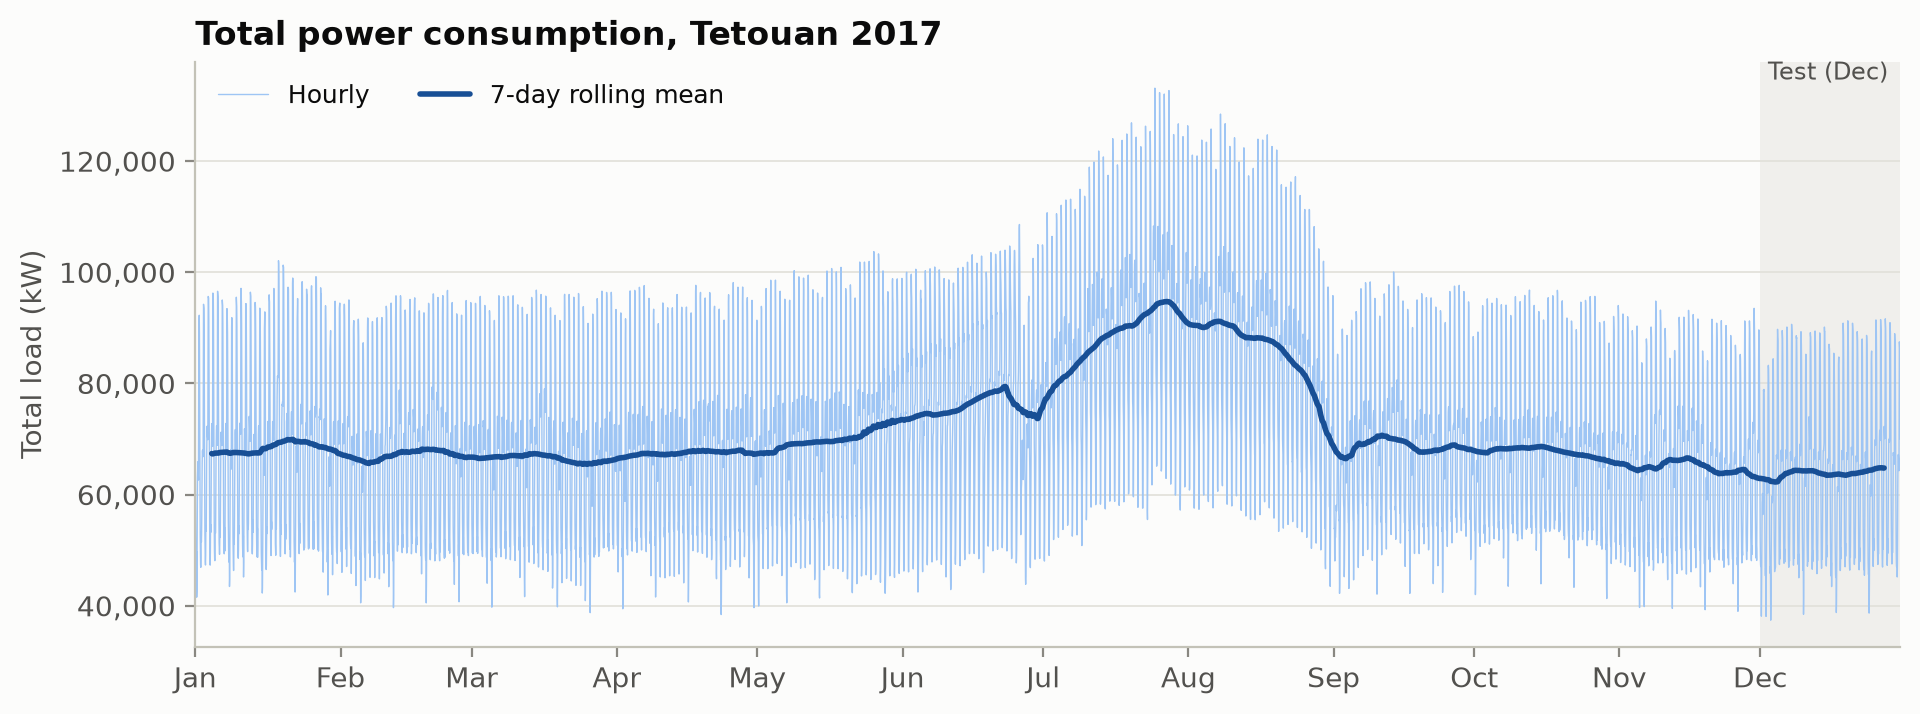
\includegraphics[width=\linewidth]{F01_total_hourly_year.png}
\caption{Hourly total load and a centered seven-day descriptive mean (F01). Summer changes the load level and amplitude. December is shaded; this whole-year plot is descriptive, and its centered mean is not a model feature.}\label{fig:annual}
\end{figure}

The zone curves in \cref{fig:zones} show that the aggregate combines different seasonal patterns. Zone 3 has a particularly large summer rise, whereas Zone 2 grows relative to Zone 3 later in the year. Such patterns motivate a city-total target for this study but do not establish the cause of each zone-level change. There are no separately trained zone models or zone forecast metrics in the saved results.
\begin{figure}[tbp]\centering
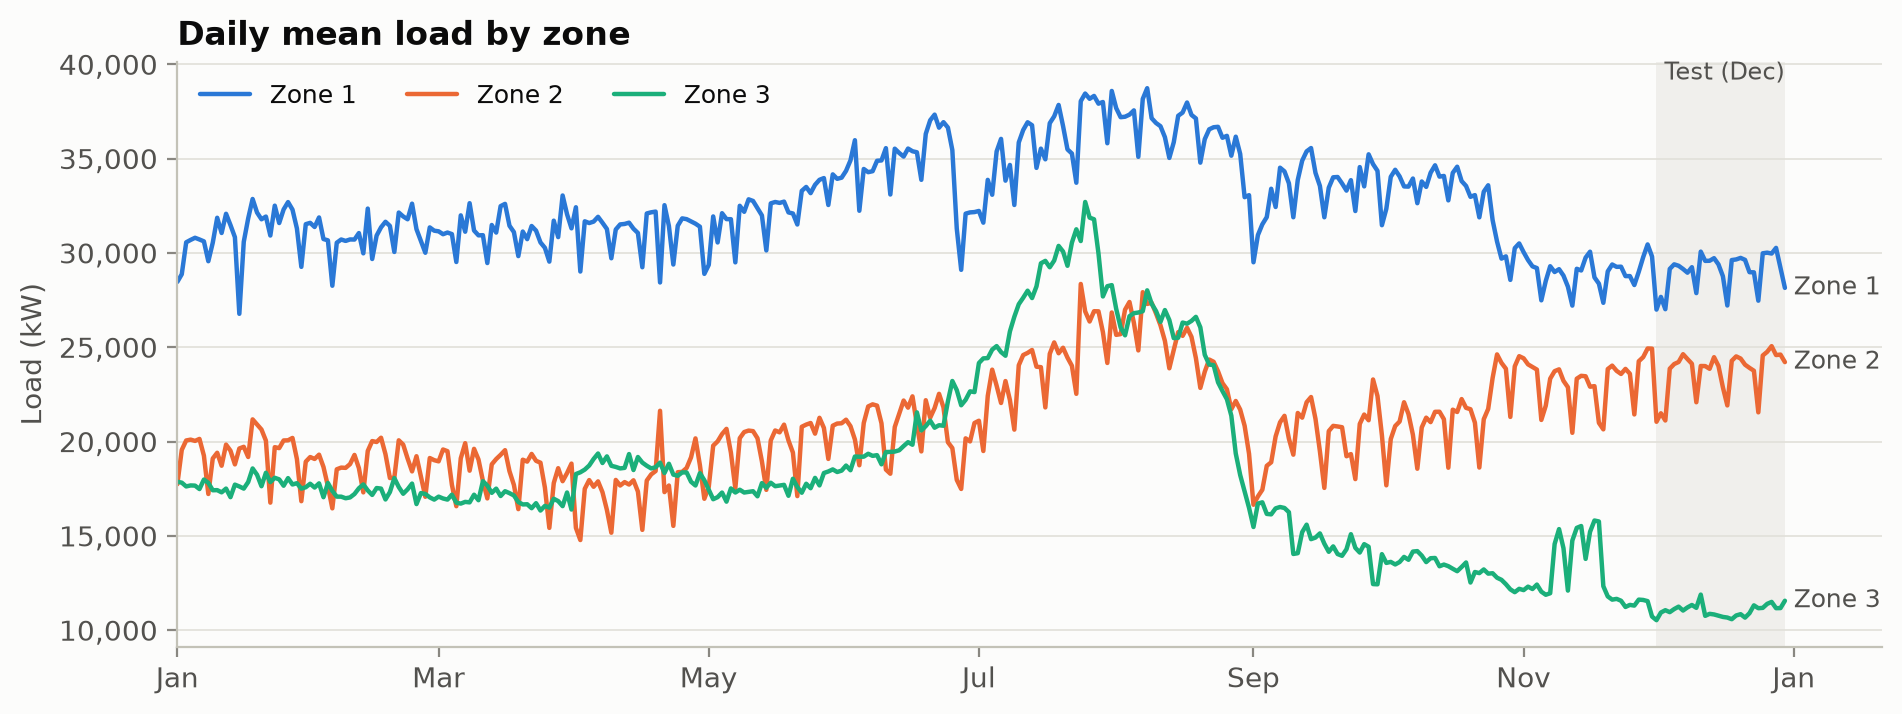
\includegraphics[width=\linewidth]{F02_zones_daily.png}
\caption{Daily means of the three distribution-zone loads (F02). Their differing seasonal behavior contributes to the changing city total. December is shown for description, not as a development validation fold.}\label{fig:zones}
\end{figure}

\subsection{Daily, weekly and special-day patterns}
The development-period seasonal profiles in \cref{fig:season} have early-morning minima around 06:00--07:00 and evening maxima around 19:00--20:00. Their peak-to-trough ratios range approximately from 1.89 to 2.11. The one-hour shift in evening peak timing is compatible with seasonal daylight and possibly clock conventions, but no timezone or daylight-saving correction is implemented.
\begin{figure}[tbp]\centering
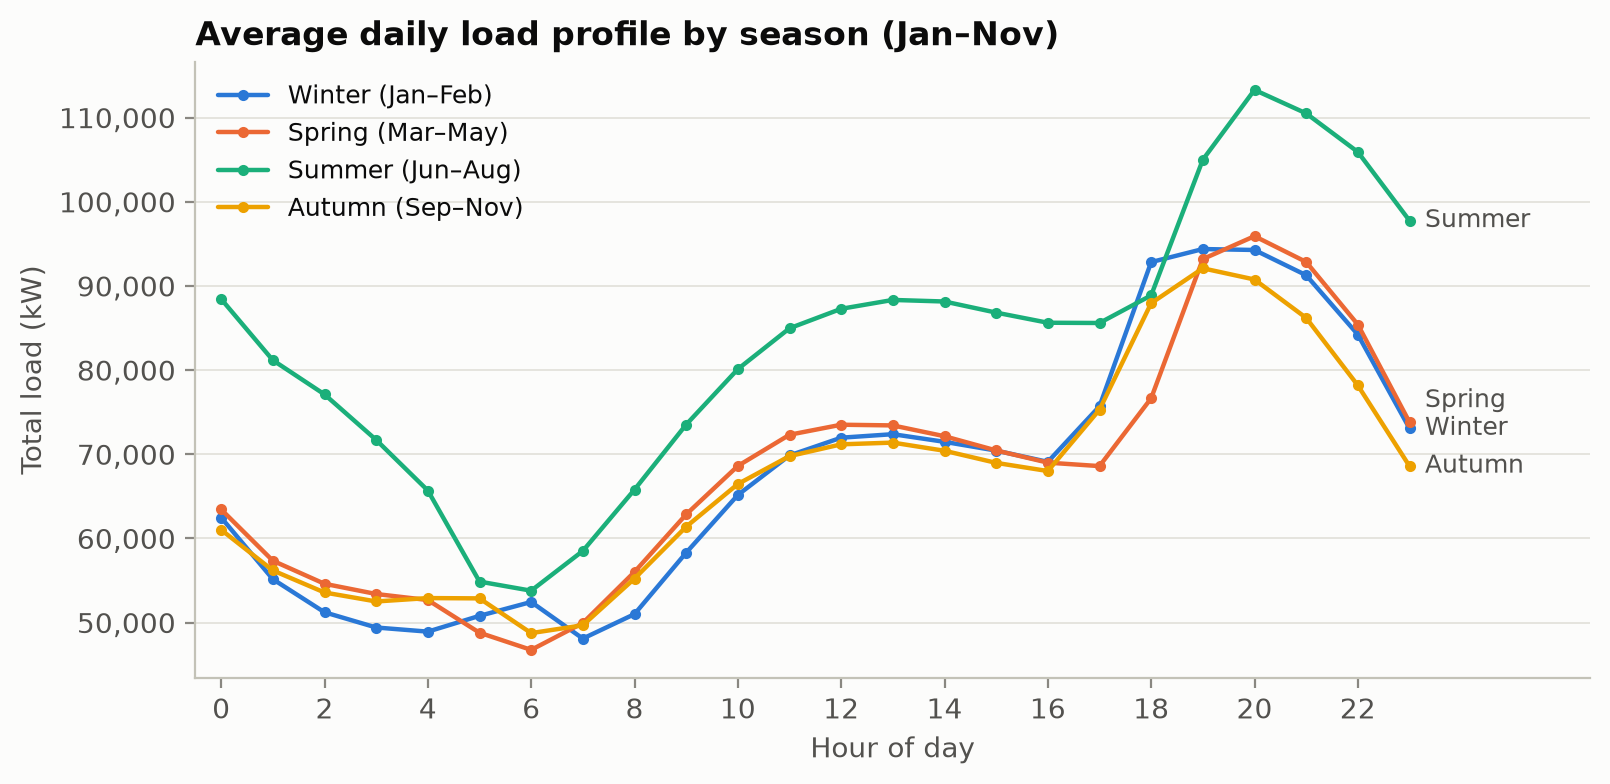
\includegraphics[width=.90\linewidth]{F03_profile_by_season.png}
\caption{Mean daily profiles by season, January--November only (F03). The common cycle motivates hour encodings; changes in level motivate historical load predictors. The chart does not isolate temperature or daylight effects.}\label{fig:season}
\end{figure}

The relative heatmap in \cref{fig:weekday} removes the large daily cycle by comparing each hour with the Monday--Friday mean of that hour. Sundays are approximately 5.9\% lower on average, with stronger early-morning deviations. This gives a specific prediction for the baseline analysis: copying Sunday's load into Monday should underestimate some Monday hours. The ML models can condition that correction on weekday and hour.
\begin{figure}[tbp]\centering
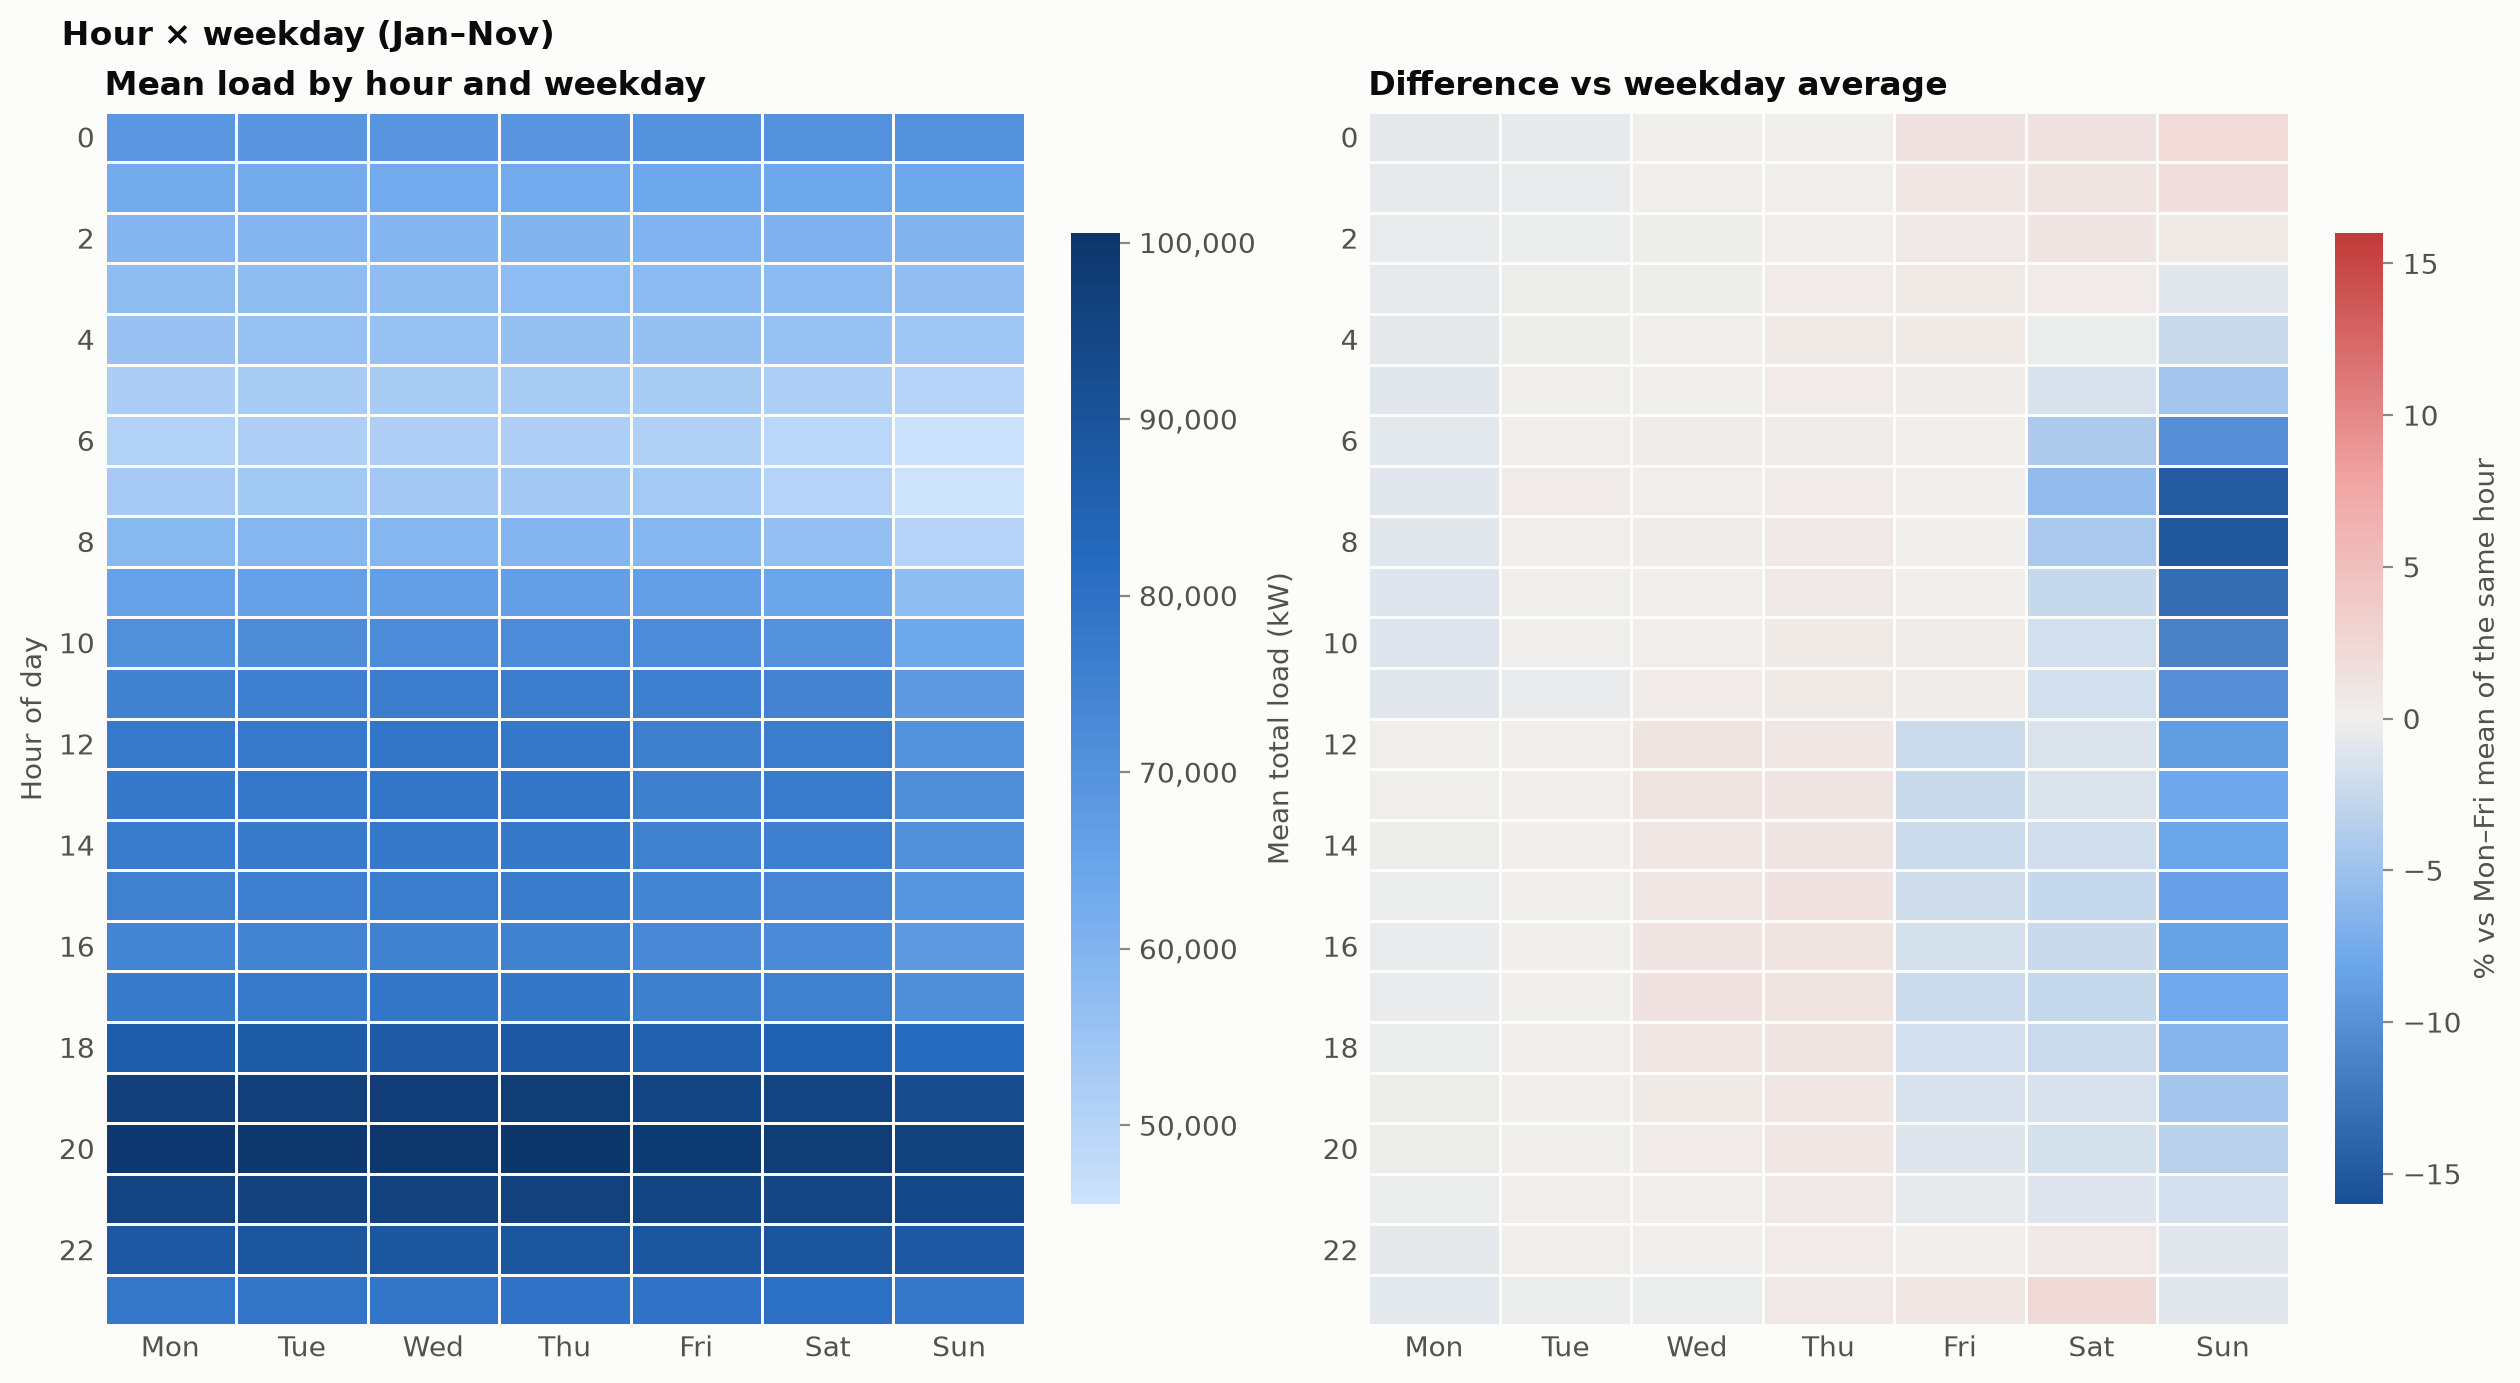
\includegraphics[width=\linewidth]{F04_heatmap_hour_weekday.png}
\caption{Development-period hour--weekday patterns (F04). The right panel expresses deviations relative to the weekday mean at the same hour, revealing variation otherwise dominated by the daily load cycle.}\label{fig:weekday}
\end{figure}

Ramadan and the preceding four weeks have distinct nighttime profiles (\cref{fig:ramadan}); the saved analysis finds a difference near \num{32142} kW at 02:00. The comparison also spans a seasonal and temperature change. It motivates a Ramadan indicator without establishing a causal effect of religious practice or ruling out weather contributions. Holiday deviations relative to a centered fifteen-day median are also heterogeneous (\cref{fig:holidays}). The repository distinguishes religious and civil holidays rather than assigning one common effect to every listed date. Centered smoothing here is descriptive EDA only.
\begin{figure}[tbp]\centering
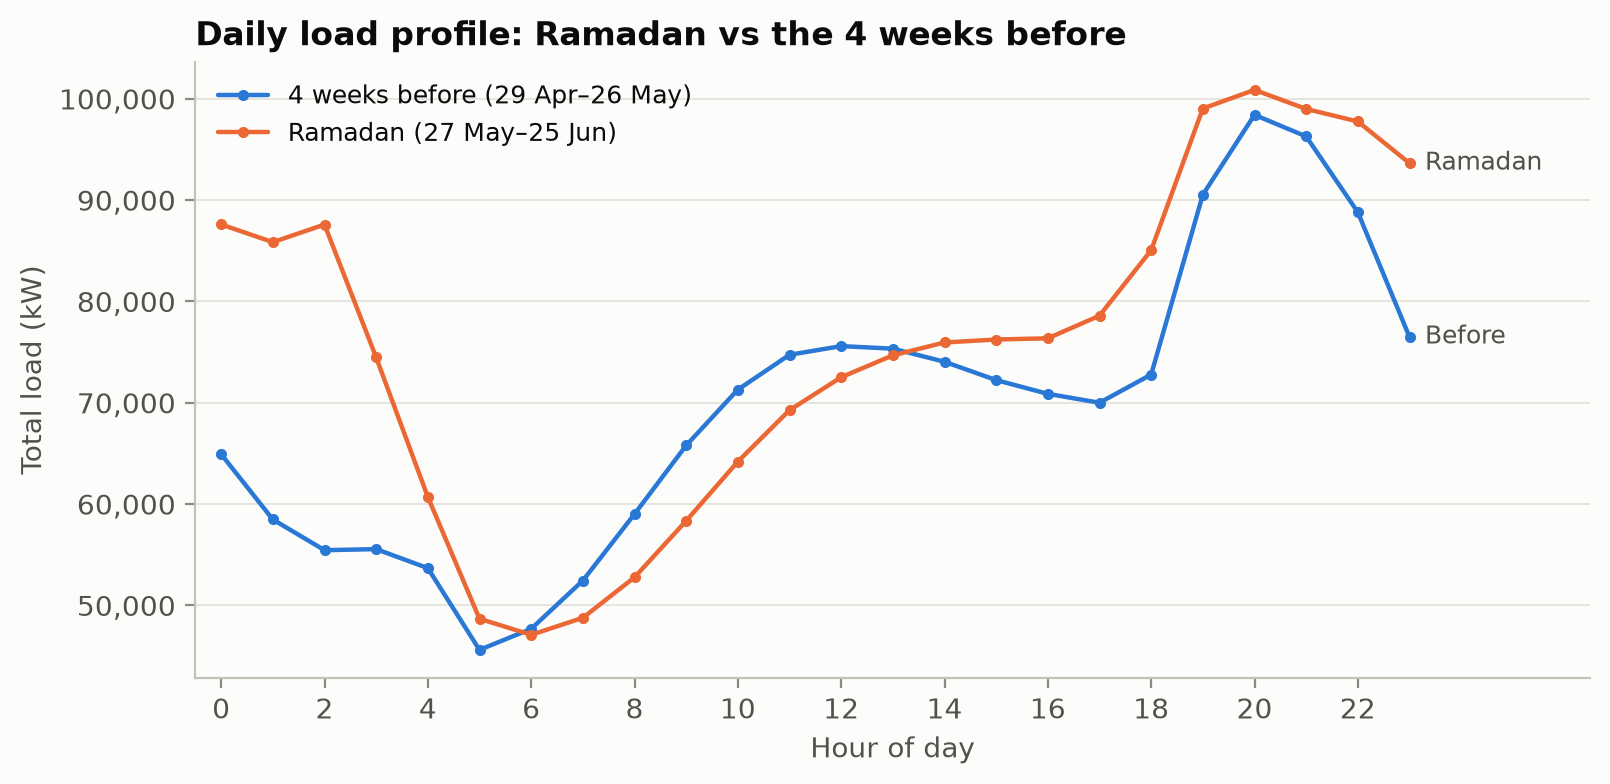
\includegraphics[width=.93\linewidth]{F05_ramadan_profile.png}
\caption{Ramadan and pre-Ramadan hourly profiles, with listed public holidays removed (F05). Large nighttime differences motivate a special-period indicator; seasonal confounding remains.}\label{fig:ramadan}
\end{figure}

\subsection{Weather association and serial dependence}
The weather scatter and correlation matrix in \cref{fig:temperature,fig:correlation} concern January--November hourly observations. Total load has Pearson correlation approximately 0.49 with temperature, $-0.30$ with humidity, 0.21 with wind speed, 0.15 with general diffuse flows and 0.02 with diffuse flows. The temperature scatter has separate time-of-day bands and a stronger high-temperature load association. These are predictive associations; they do not identify cooling consumption separately or demonstrate that weather effects are absent at lower temperatures.
\begin{figure}[tbp]\centering
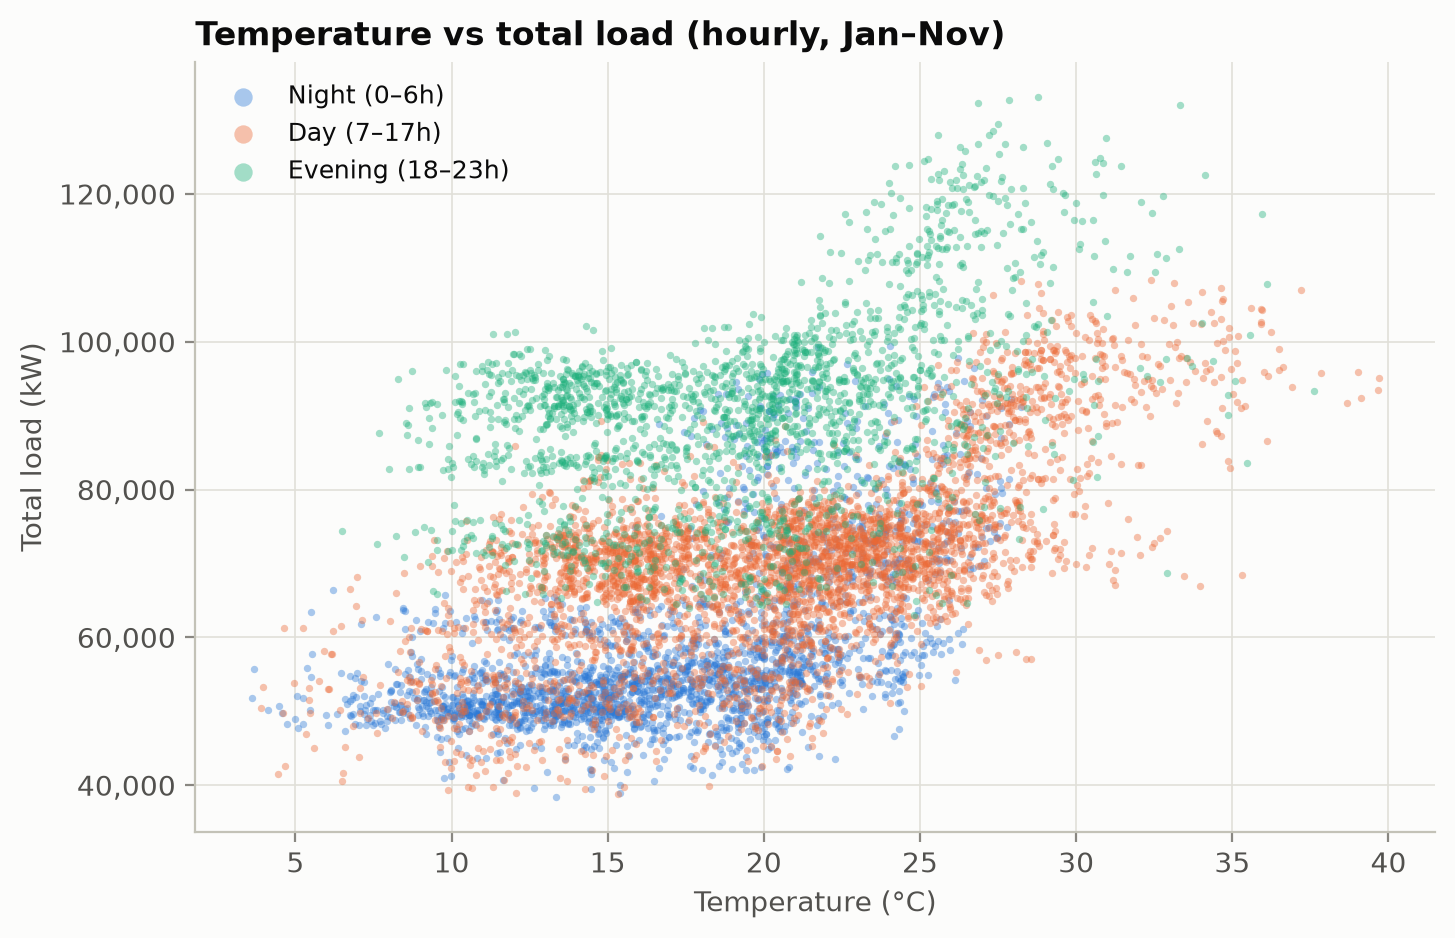
\includegraphics[width=.80\linewidth]{F06a_temperature_vs_total.png}
\caption{Target-hour temperature and total load, colored by time of day (F06a). Distinct bands indicate that calendar conditioning is relevant when interpreting the weather--load relationship.}\label{fig:temperature}
\end{figure}
\begin{figure}[tbp]\centering
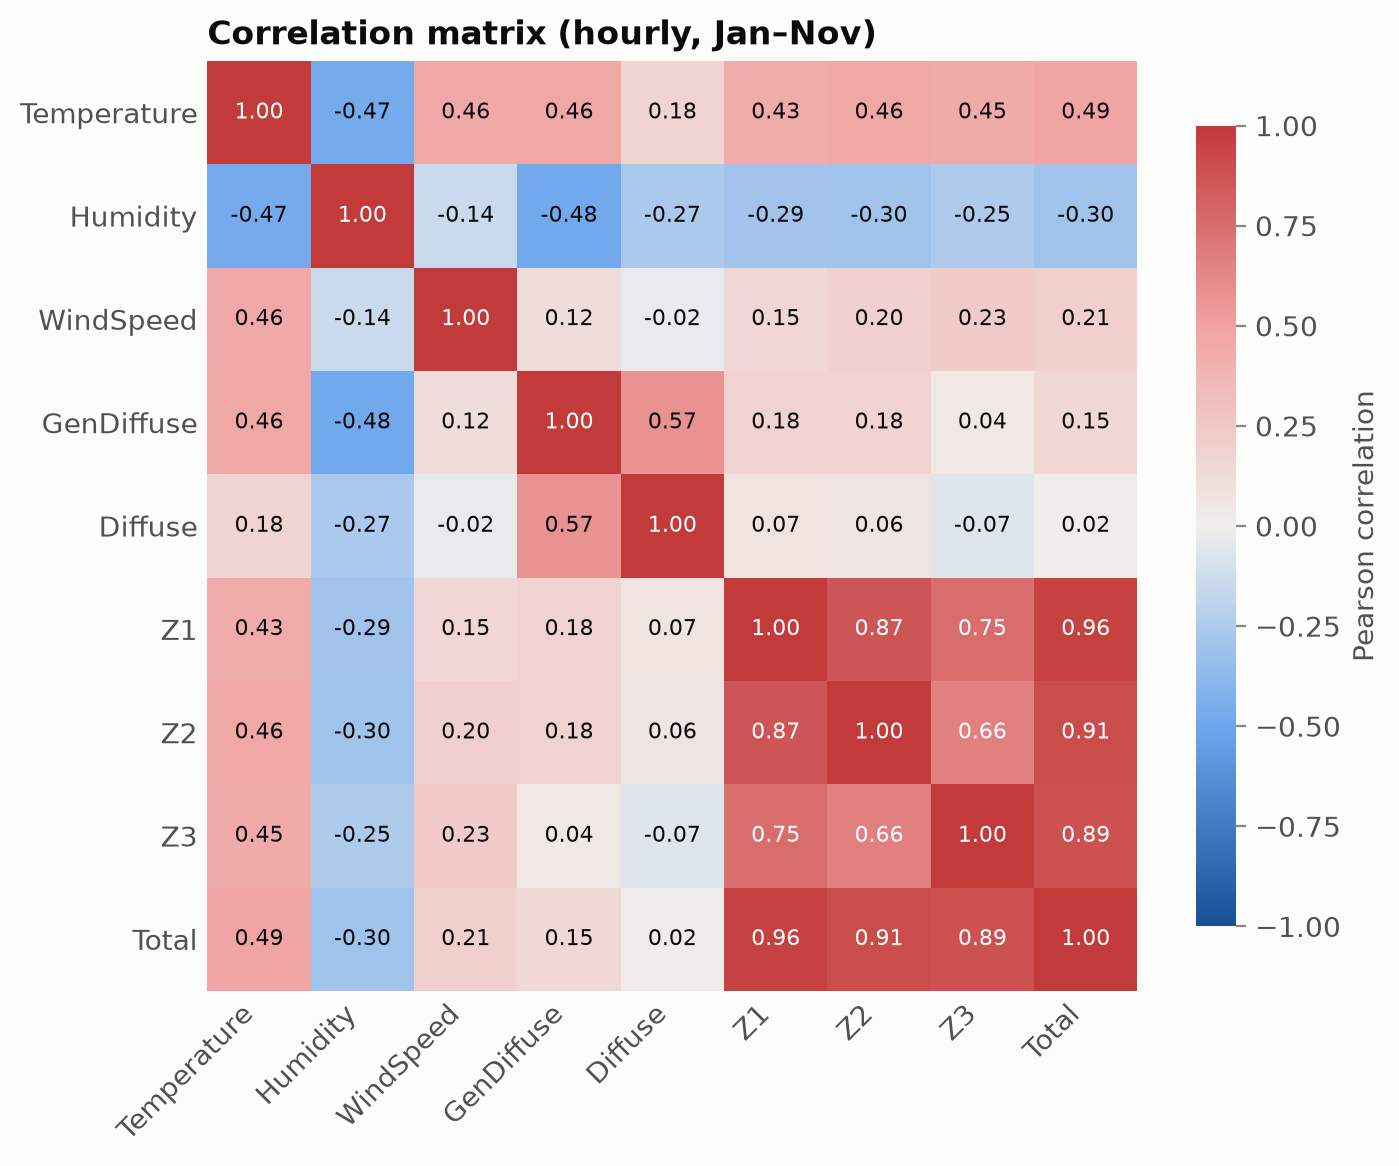
\includegraphics[width=.77\linewidth]{F06b_correlation.png}
\caption{Pearson correlations on hourly development data (F06b). Strong correlations between zones and their sum are expected arithmetically; contemporaneous zones are excluded as forecasting inputs.}\label{fig:correlation}
\end{figure}

The autocorrelation in \cref{fig:acf} is approximately 0.98 at lag 24 and 0.95 at lag 168, with recurring daily peaks. These findings motivate seasonal lags and a previous-day baseline. High autocorrelation does not determine the optimal feature set: a weekly predictor may still hurt a particular fitted model under a changing load regime, as the ablation later demonstrates. The plotted ACF bands are not forecast intervals.
\begin{figure}[tbp]\centering
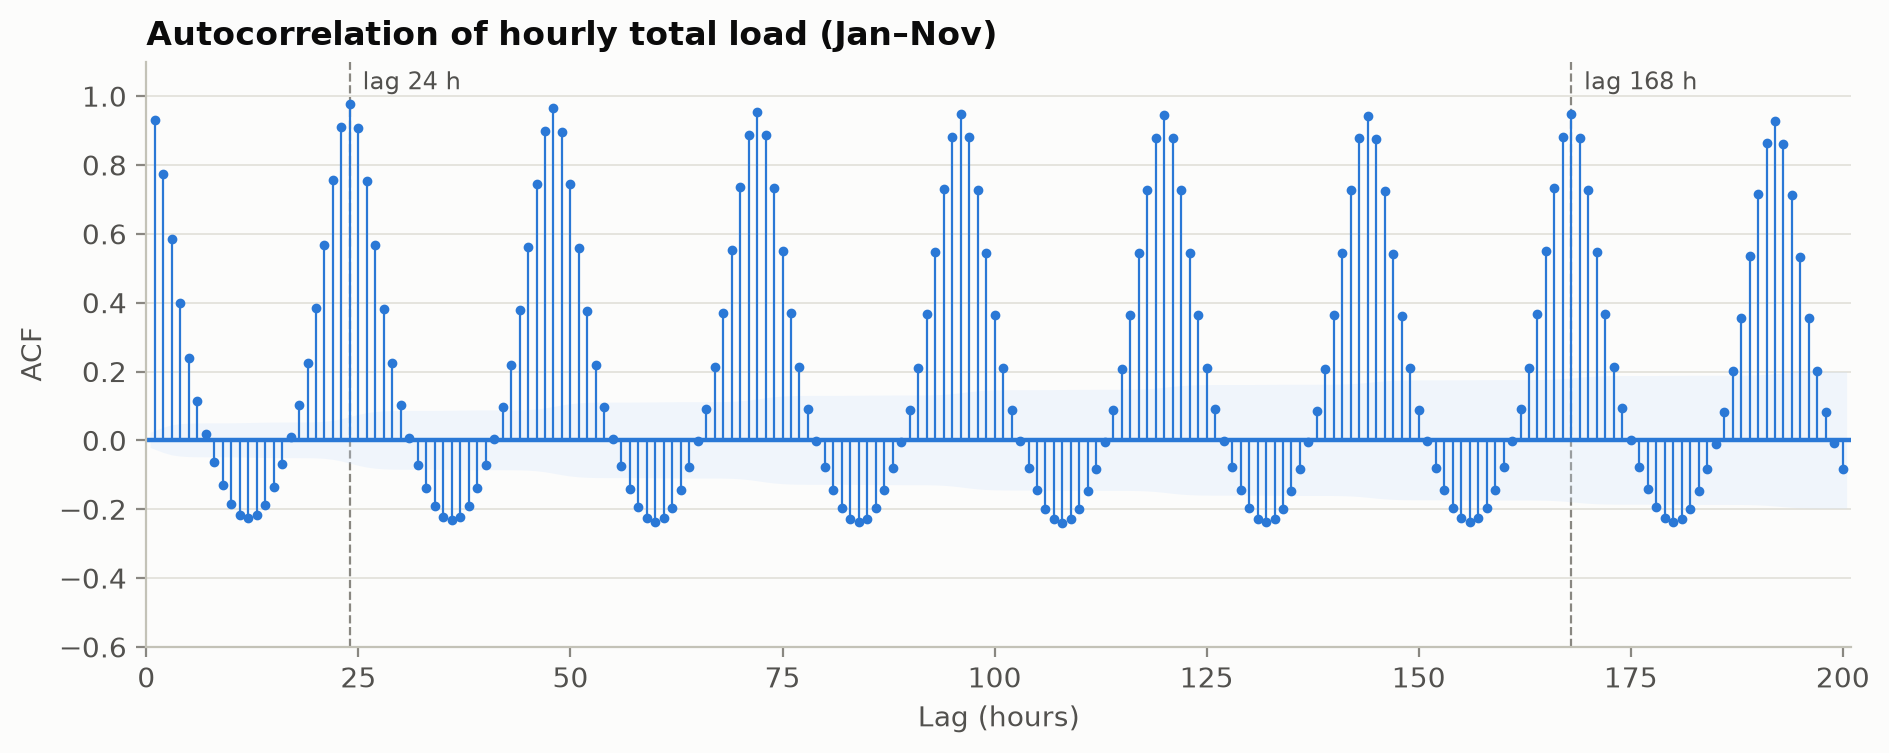
\includegraphics[width=\linewidth]{F07_acf_total.png}
\caption{Autocorrelation of the hourly total through 200 lags, January--November (F07). Daily and weekly dependence motivate history-based predictors and make randomly shuffled evaluation a poor proxy for future forecasting.}\label{fig:acf}
\end{figure}
\evidence{Notebook 01 cells 4--43; T01 data-quality/descriptive tables; F01--F08; DQ01--DQ02. F03--F08 use development data; F01/F02 and DQ02 include December.}

\section{Data Preprocessing and Feature Engineering}\label{sec:features}
\subsection{Chronological data construction}
The loader renames the nine CSV columns by position, parses timestamps explicitly as month/day/year and hour:minute, sets the datetime index, and sorts it. No timezone is assigned. Let $z_{j,s}$ be the recorded load for zone $j$ at ten-minute timestamp $s$. The raw total and hourly target are
\begin{equation}
q_s=\sum_{j=1}^{3}z_{j,s},\qquad
y_t=\frac{1}{6}\sum_{r=0}^{5}q_{t+10r\,\mathrm{min}}.
\label{eq:target}
\end{equation}
Weather columns are averaged over the same hourly bin. The timestamp labels the start of the bin; its mean becomes available only after its observations have been collected. No outlier replacement or interpolation is performed. Although pandas averaging could skip missing observations in a different dataset, the saved quality check finds complete bins here; the pipeline should not be interpreted as implementing a general missing-data policy.

\subsection{Calendar and special-day encoding}
The main feature builder includes raw hour $a_t\in\{0,\ldots,23\}$, weekday $d_t\in\{0,\ldots,6\}$ and a weekend indicator $\mathbb{1}(d_t\ge5)$. Cyclic encodings supplement rather than replace the raw fields:
\begin{equation}
\left[\sin\!\left(\frac{2\pi a_t}{24}\right),\cos\!\left(\frac{2\pi a_t}{24}\right),
\sin\!\left(\frac{2\pi d_t}{7}\right),\cos\!\left(\frac{2\pi d_t}{7}\right)\right].
\label{eq:calendar}
\end{equation}
These variables are known for future target intervals. Separate binary indicators encode civil holidays, religious holidays and Ramadan. The implemented Ramadan interval is 27 May through 25 June, using an exclusive end date of 26 June. The holiday lists are fixed for 2017. Their calendar provenance is not separately archived; the development EDA was used to assess their load associations. Deployment in another year would require a maintained calendar.

\subsection{Lag and rolling features}
For horizon parameter $h$, the builder creates historical load features
\begin{equation}
\ell_k(t)=y_{t-k},\qquad k\ge h.
\label{eq:lags}
\end{equation}
The built lags are $\{24,48,168\}$ for \hday\ and $\{1,2,3,24,168\}$ for \hone. Rolling features are calculated \emph{after} shifting by $h$:
\begin{align}
\mu_{w,h}(t)&=\frac{1}{w}\sum_{j=0}^{w-1}y_{t-h-j},\quad w\in\{24,168\},\label{eq:rollingmean}\\
s_{24,h}(t)&=\sqrt{\frac{1}{23}\sum_{j=0}^{23}\left(y_{t-h-j}-\mu_{24,h}(t)\right)^2}.
\label{eq:rollingstd}
\end{align}
The denominator in \cref{eq:rollingstd} follows pandas' sample-standard-deviation default. No window includes $y_t$. The feature checker recomputes lag and rolling values at 200 sampled timestamps for each horizon; notebook 02 also deliberately inserts an unshifted rolling mean and confirms detection. This verifies temporal construction of load-history columns, not the availability of the weather columns.

\subsection{Built features versus selected inputs}
\Cref{tab:features} distinguishes constructed columns from model inputs. The main \hday\ models use set D, with 17 columns. The \hone\ models use 19 columns, replacing the daily-lag pair with lags 1, 2, 3 and 24. Weekly and rolling columns remain available for naive baselines and ablation experiments.
\begin{table}[tbp]\centering\small
\caption{Implemented feature groups and prediction-time availability. The target-hour weather values are observed rather than forecast.}\label{tab:features}
\begin{tabularx}{\linewidth}{@{}p{.18\linewidth}Xp{.22\linewidth}@{}}\toprule
Group & Construction and use & Availability \\\midrule
Weather (5) & Temperature, humidity, wind speed, general diffuse flows, diffuse flows; both horizons & Oracle target-hour weather \\
Calendar (7) & Hour, weekday, weekend flag and four sine/cosine encodings; both horizons & Known calendar \\
Special days (3) & Religious holiday, civil holiday, Ramadan; both horizons & Fixed 2017 calendar \\
Daily lags (2) & $y_{t-24}$, $y_{t-48}$; selected for h24 & Previous completed days \\
Recent/daily lags (4) & $y_{t-1}$, $y_{t-2}$, $y_{t-3}$, $y_{t-24}$; selected for h1 & Updated completed hours \\
Weekly/rolling (4) & $y_{t-168}$, $\mu_{24,h}$, $s_{24,h}$, $\mu_{168,h}$; constructed, excluded from main inputs & Past windows only \\
\bottomrule\end{tabularx}
\end{table}

The complete matrices contain 21 and 23 columns, respectively. The builder joins all features with the response and drops any incomplete row \emph{before} selecting D or the h1 subset. Consequently, unused weekly/rolling features still determine the initial warm-up loss: 191 hours for \hday\ and 168 for \hone. This leaves \num{8545} and \num{8568} eligible rows. The first \hday\ row is 8 January at 23:00, and the first \hone\ row is 8 January at 00:00. No later observations are removed in this dataset.

\subsection{Issuance and information availability}
At midnight of day $D$, yesterday's same-hour load is available for every target interval in day $D$, assuming completed-hour measurements are delivered promptly. The latest such interval is yesterday at 23:00. Thus the daily batch can use all selected load-history features without recursively predicting intermediate loads. However, its intervals begin 0--23 hours after midnight; the repository label \hday\ denotes a minimum history lag, not a uniform 24-hour lead for every forecast. No explicit scheduler or issuance-time dataset is implemented.

In the hourly setting, the immediately previous completed hour is used to predict the next interval. The evaluation updates these measured histories as time advances, including within validation and test months. It does not forecast the entire December trajectory using only information available on 1 December.

Weather is different: \code{X = dh[WEATHER].copy()} takes the realized mean weather during the interval being forecast. These values are not available at issuance. The results therefore answer a conditional forecasting question with perfect weather information. A deployment study would need archived weather forecasts or an alternative available-information design. The selected-SVR effect of that replacement is not measured here.

\subsection{Scaling and lag-relative targets}
Linear regression and Ridge use training-fitted input standardization. SVR additionally standardizes the response through a transformed-target wrapper; inverse transformation returns forecasts to kW. Fitting occurs inside each CV training fold. Tree models receive the original feature scales.

For the residual formulation, \code{DeltaTarget} trains a regressor $g$ on a difference from an available base:
\begin{equation}
r_t=y_t-b_t,\qquad \widehat y_t=b_t+g(\mathbf{x}_t),\qquad
b_t=\begin{cases}y_{t-24},&\hday,\\y_{t-1},&\hone.\end{cases}
\label{eq:delta}
\end{equation}
The base remains a predictor as well. This formulation asks the model to correct a known load level, which can reduce the difficulty of predicting a new absolute level. It does not guarantee that future residuals remain in the training range. In residual SVR, the scaler is fitted to the residual target; the unscaled base is added after prediction.
\evidence{\code{src/data.py}; \code{src/features.py}; \code{src/models.py}; notebook 02 cells 3--10, 20--27; T02/T03.}

\section{Experimental Methodology}\label{sec:method}
\subsection{Prediction problem and experimental stages}
Each estimator maps a feature row $\mathbf{x}_t$ to one hourly total $\widehat y_t$. One pooled model serves all target hours within a setting, rather than 24 separate lead-specific estimators. The baseline, default, tuned and ablation comparisons share eligible target timestamps within their respective settings.

The staged protocol is: L0/L1 establish seasonal baselines and default regressors on November; L2 applies default models to five temporal folds; L3 searches parameters and compares absolute/residual targets on those same folds; notebook 06 tests feature subsets and separately tunes h1; notebook 07 refits on development data and evaluates December; notebook 08 performs post-final diagnostic experiments. The stages are a final organization of the code, not a claim that feature choices were made only once. The development history records iterative feature and target choices followed by reruns of earlier stages.

\subsection{Partitions and expanding-window validation}
The fixed boundaries are 1 November and 1 December 2017. Training for L1 ends on 31 October; November is its validation month. Development combines those two periods. Test observations span 1--30 December. \Cref{tab:splits} gives actual sample counts after warm-up. The h1 development set has 23 more early January hours because of its shorter warm-up; the validation and test periods are identical.
\begin{table}[tbp]\centering\small
\caption{Chronological partitions after history-related row removal (T02). All dates are in 2017; end times are 23:00.}\label{tab:splits}
\setlength{\tabcolsep}{4pt}
\begin{tabular}{llrrr}
\toprule
Setting & Partition & Start & End & Hours \\
\midrule
h24 & Train & 01-08 23:00 & 10-31 23:00 & \num{7105} \\
h24 & Validation & 11-01 00:00 & 11-30 23:00 & \num{720} \\
h24 & Development & 01-08 23:00 & 11-30 23:00 & \num{7825} \\
h24 & Test & 12-01 00:00 & 12-30 23:00 & \num{720} \\
h1 & Train & 01-08 00:00 & 10-31 23:00 & \num{7128} \\
h1 & Validation & 11-01 00:00 & 11-30 23:00 & \num{720} \\
h1 & Development & 01-08 00:00 & 11-30 23:00 & \num{7848} \\
h1 & Test & 12-01 00:00 & 12-30 23:00 & \num{720} \\
\bottomrule\end{tabular}
\end{table}


\code{TimeSeriesSplit(n_splits=5, test_size=720)} creates five expanding training windows with 30-day validation windows\cite{tscv}. \Cref{tab:folds,fig:split} make the boundaries explicit. The last fold exactly reproduces the L1 train/November validation partition. Fold numbering starts at zero, matching the saved tables.
\begin{table}[H]\centering\small
\caption{Expanding-window h24 cross-validation (T02). Training starts on 8 January at 23:00 in every fold; validation begins at 00:00 and ends at 23:00.}\label{tab:folds}
\setlength{\tabcolsep}{4pt}
\begin{tabular}{rlrll}
\toprule
Fold & Training ends & Train hours & Validation starts & Validation ends \\
\midrule
\num{0} & 2017-07-03 & \num{4225} & 2017-07-04 & 2017-08-02 \\
\num{1} & 2017-08-02 & \num{4945} & 2017-08-03 & 2017-09-01 \\
\num{2} & 2017-09-01 & \num{5665} & 2017-09-02 & 2017-10-01 \\
\num{3} & 2017-10-01 & \num{6385} & 2017-10-02 & 2017-10-31 \\
\num{4} & 2017-10-31 & \num{7105} & 2017-11-01 & 2017-11-30 \\
\bottomrule\end{tabular}
\end{table}

\begin{figure}[tbp]\centering
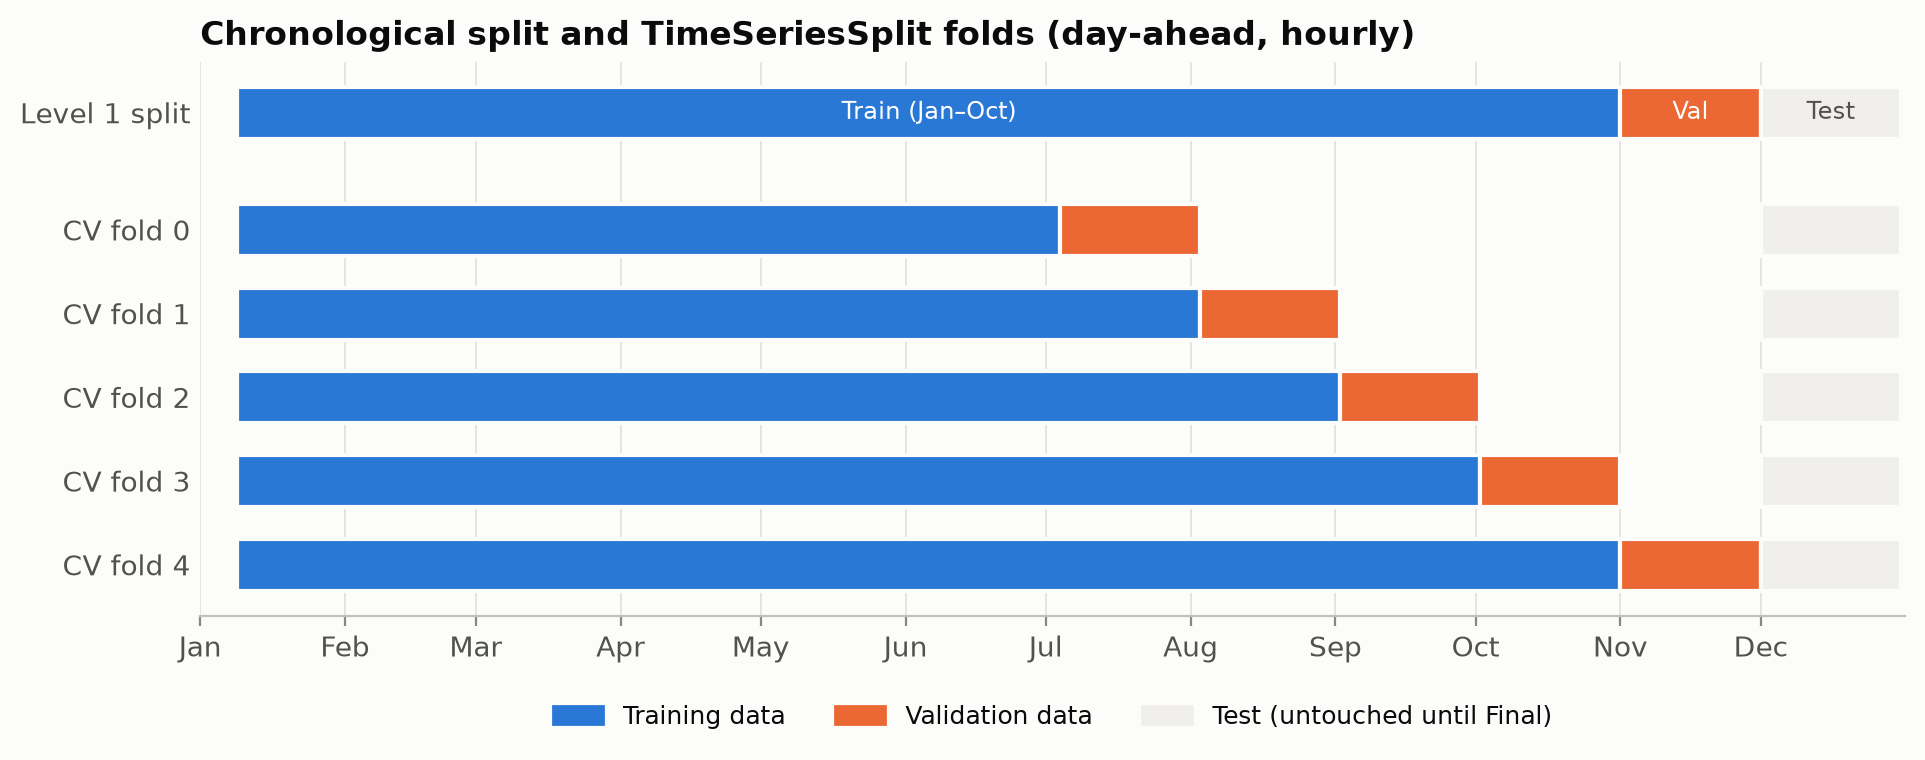
\includegraphics[width=\linewidth]{F10_split_and_folds.png}
\caption{Chronological partitions and five expanding validation folds (F10). December is outside model-selection folds. The original graphic's ``untouched'' wording describes the intended partition; whole-year descriptive EDA and later test reruns qualify literal unseen-data claims.}\label{fig:split}
\end{figure}

No gap is specified, so the implementation uses zero gap. Under the midnight interpretation, completed prior-day labels can be available when the next validation day begins; load-history columns do not access later target-day loads. This assumes negligible collection and model-fitting latency. It does not establish the validity of a different issuance time, nor does it resolve unavailable future weather. The repository contains no saved comparison with a nonzero gap.

The model is fitted once per fold and evaluated with measured historical loads updating through the validation window. This differs from an open-loop forecast of all 720 hours at the fold boundary. Fold SD reflects changing regimes and training sizes. Overlapping training sets and dependent hourly errors mean it is not a standard error of five independent estimates.

\subsection{Baselines and model families}
The seasonal baselines are $\widehat y_t=y_{t-24}$ and $\widehat y_t=y_{t-168}$. MeanProfile estimates the training mean for $(a_t,d_t)$, with the training global mean as a fallback for an absent combination. The h1 persistence baseline uses $y_{t-1}$. Baselines are evaluated on the same rows as ML models, using the full constructed feature matrix where necessary.

The default model implementations are standardized ordinary least squares, an unconstrained decision tree, a 100-tree random forest, standardized RBF SVR with target scaling, and XGBRegressor. Stochastic estimators use seed 42. RF-P1 uses 30 trees and seven candidate features per split, with unrestricted depth, minimum split size two and minimum leaf size one. This imports a literature configuration into the current pipeline; it is not a reproduction of that paper's complete experiment.

In L3, the LR label denotes Ridge, and each family has an absolute and residual version. Parameters not explicitly set are inherited from the repository's pinned libraries. \Cref{sec:tuning} gives the search details. No additional forecasting family is silently introduced.

\subsection{Metrics and aggregation}
For $n$ evaluated hours with observations $y_i$, forecasts $\widehat y_i$ and evaluation-set mean $\bar y$, the implemented metrics are
\begin{align}
\mathrm{MAE}&=\frac{1}{n}\sum_{i=1}^{n}|y_i-\widehat y_i|,\\
\mathrm{RMSE}&=\sqrt{\frac{1}{n}\sum_{i=1}^{n}(y_i-\widehat y_i)^2},\\
\mathrm{MAPE}&=\frac{100}{n}\sum_{i=1}^{n}\left|\frac{y_i-\widehat y_i}{y_i}\right|,\\
R^2&=1-\frac{\sum_i(y_i-\widehat y_i)^2}{\sum_i(y_i-\bar y)^2}.
\label{eq:metrics}
\end{align}
RMSE emphasizes large errors; MAE measures average absolute deviation. MAPE weights errors relative to each actual load and is reported in percent. The custom implementation has no special zero-target treatment, but observed loads are positive. R$^2$ depends on the variance of the evaluation period, so differences across settings require care.

CV reports the arithmetic mean of five fold metrics and sample SD. Mean fold RMSE is generally different from RMSE pooled over all fold predictions, even with equal fold sizes. Likewise, mean fold R$^2$ is not pooled R$^2$. Search-result SDs use a population convention internally; this report's displayed fold SD follows the saved pandas summaries.

The baseline-relative skill is
\begin{equation}
S=1-\frac{\mathrm{RMSE}_{model}}{\mathrm{RMSE}_{Naive24}}.
\label{eq:skill}
\end{equation}
Positive skill indicates improvement; negative skill indicates worse RMSE. The L2 and ablation summaries average fold-specific skills, while the tuning comparison includes a ratio of mean RMSEs. Those summaries should not be interchanged. December skill compares metrics on the same 720 hours. Additional diagnostics include signed bias, error by hour/day, runtime and validation-to-training RMSE ratio; none replaces mean CV RMSE as the selection objective.

\subsection{Selection and evaluation limitations}
The final h24 identity is the minimum mean L3 CV RMSE among tuned variants. The final h1 identity follows its separate development search. Both select absolute-target SVR. Although notebook 07 computes a test table before printing the chosen name, the choice expression reads only development CV results. The static code therefore supports the stated selection rule, but is not a prospective registration of the development process.

Feature selection, holiday interpretation, residual-base selection and parameter optimization reuse January--November observations. No nested outer CV or correction for repeated selection is implemented. Whole-year descriptive EDA exposes the test month; progress notes also report later unchanged-pipeline reruns. The appropriate description is a separate chronological test period under a documented CV selection rule, with limits to one-shot independence. No significance test, calibration analysis or predictive interval is reported.
\evidence{\code{src/config.py}; \code{src/evaluate.py}; \code{src/models.py}; T02; notebooks 03--08; \code{docs/progress.md}.}

\section{Baseline Experiments}\label{sec:baseline}
\subsection{Objective and common evaluation conditions}
Notebook 03 establishes whether the selected predictors support improvement over simple load-history rules before hyperparameter search. All h24 candidates use the same \num{7105} training hours ending on 31 October and the same 720 November validation hours. The five default ML models use the 17-column set D defined in \cref{sec:features}; the baselines access their required historical columns on the same eligible timestamps. This comparison measures performance in November, rather than accuracy averaged across seasonal regimes.

Naive-24h and Naive-168h copy the preceding day's and preceding week's corresponding hour. Their usefulness follows from the daily and weekly dependence in \cref{fig:acf}. MeanProfile instead pools the training observations associated with each hour and weekday. Writing $I_{a,d}=\{i\in\mathcal T:a_i=a,\ d_i=d\}$ for the training subset, its prediction is
\begin{equation}
\widehat y_t^{\mathrm{profile}}=\begin{cases}
|I_{a_t,d_t}|^{-1}\displaystyle\sum_{i\in I_{a_t,d_t}}y_i,&|I_{a_t,d_t}|>0,\\
|\mathcal T|^{-1}\displaystyle\sum_{i\in\mathcal T}y_i,&\text{otherwise}.
\end{cases}\label{eq:meanprofile}
\end{equation}
The profile and its fallback are fitted only to training observations. The seasonal rules have no fitted coefficients, although their histories update as measured loads become available.

The additional RF-P1 configuration has 30 trees and seven candidate features per split, with unrestricted depth and the split/leaf minima specified in \cref{sec:method}. Its role is to test a literature-inspired parameter configuration within this project's target and validation design. It does not establish replication of an external paper's scores.

\subsection{November results}
\Cref{tab:baselines,fig:baseline_comparison} show the saved comparison. XGB has the lowest validation RMSE, \num{2161.4} kW, and also the lowest MAE and MAPE, \num{1598.4} kW and \num{2.42}\%, respectively. Against Naive-24h at \num{3076.4} kW RMSE, its RMSE reduction is \num{29.74}\%. RF-P1, SVR and RF follow at \num{2192.0}, \num{2195.2} and \num{2227.5} kW. These relatively close November results do not establish statistically significant differences.
\begin{table}[tbp]\centering\small
\caption{November validation, h24: seasonal baselines, default regressors and RF-P1 (T04). RMSE/MAE are in kW; MAPE is percent.}\label{tab:baselines}
\setlength{\tabcolsep}{4pt}
\begin{tabular}{lrrrrr}
\toprule
Model & Train RMSE & Val. RMSE & Val. MAE & MAPE & R$^2$ \\
\midrule
XGB & \num{812.4} & \num{2161.4} & \num{1598.4} & \num{2.42} & \num{0.9760} \\
RF-P1 & \num{805.0} & \num{2192.0} & \num{1620.3} & \num{2.50} & \num{0.9753} \\
SVR & \num{1567.7} & \num{2195.2} & \num{1601.1} & \num{2.52} & \num{0.9753} \\
RF & \num{794.4} & \num{2227.5} & \num{1616.7} & \num{2.47} & \num{0.9745} \\
LR & \num{2670.5} & \num{2288.7} & \num{1734.0} & \num{2.76} & \num{0.9731} \\
DT & \num{0.0} & \num{2992.4} & \num{2190.0} & \num{3.34} & \num{0.9540} \\
Naive-24h & \num{3497.5} & \num{3076.4} & \num{2080.7} & \num{3.27} & \num{0.9514} \\
Naive-168h & \num{4686.4} & \num{3202.9} & \num{2425.8} & \num{3.79} & \num{0.9473} \\
MeanProfile & \num{9628.3} & \num{9369.6} & \num{8560.8} & \num{13.50} & \num{0.5493} \\
\bottomrule\end{tabular}
\end{table}

\begin{figure}[tbp]\centering
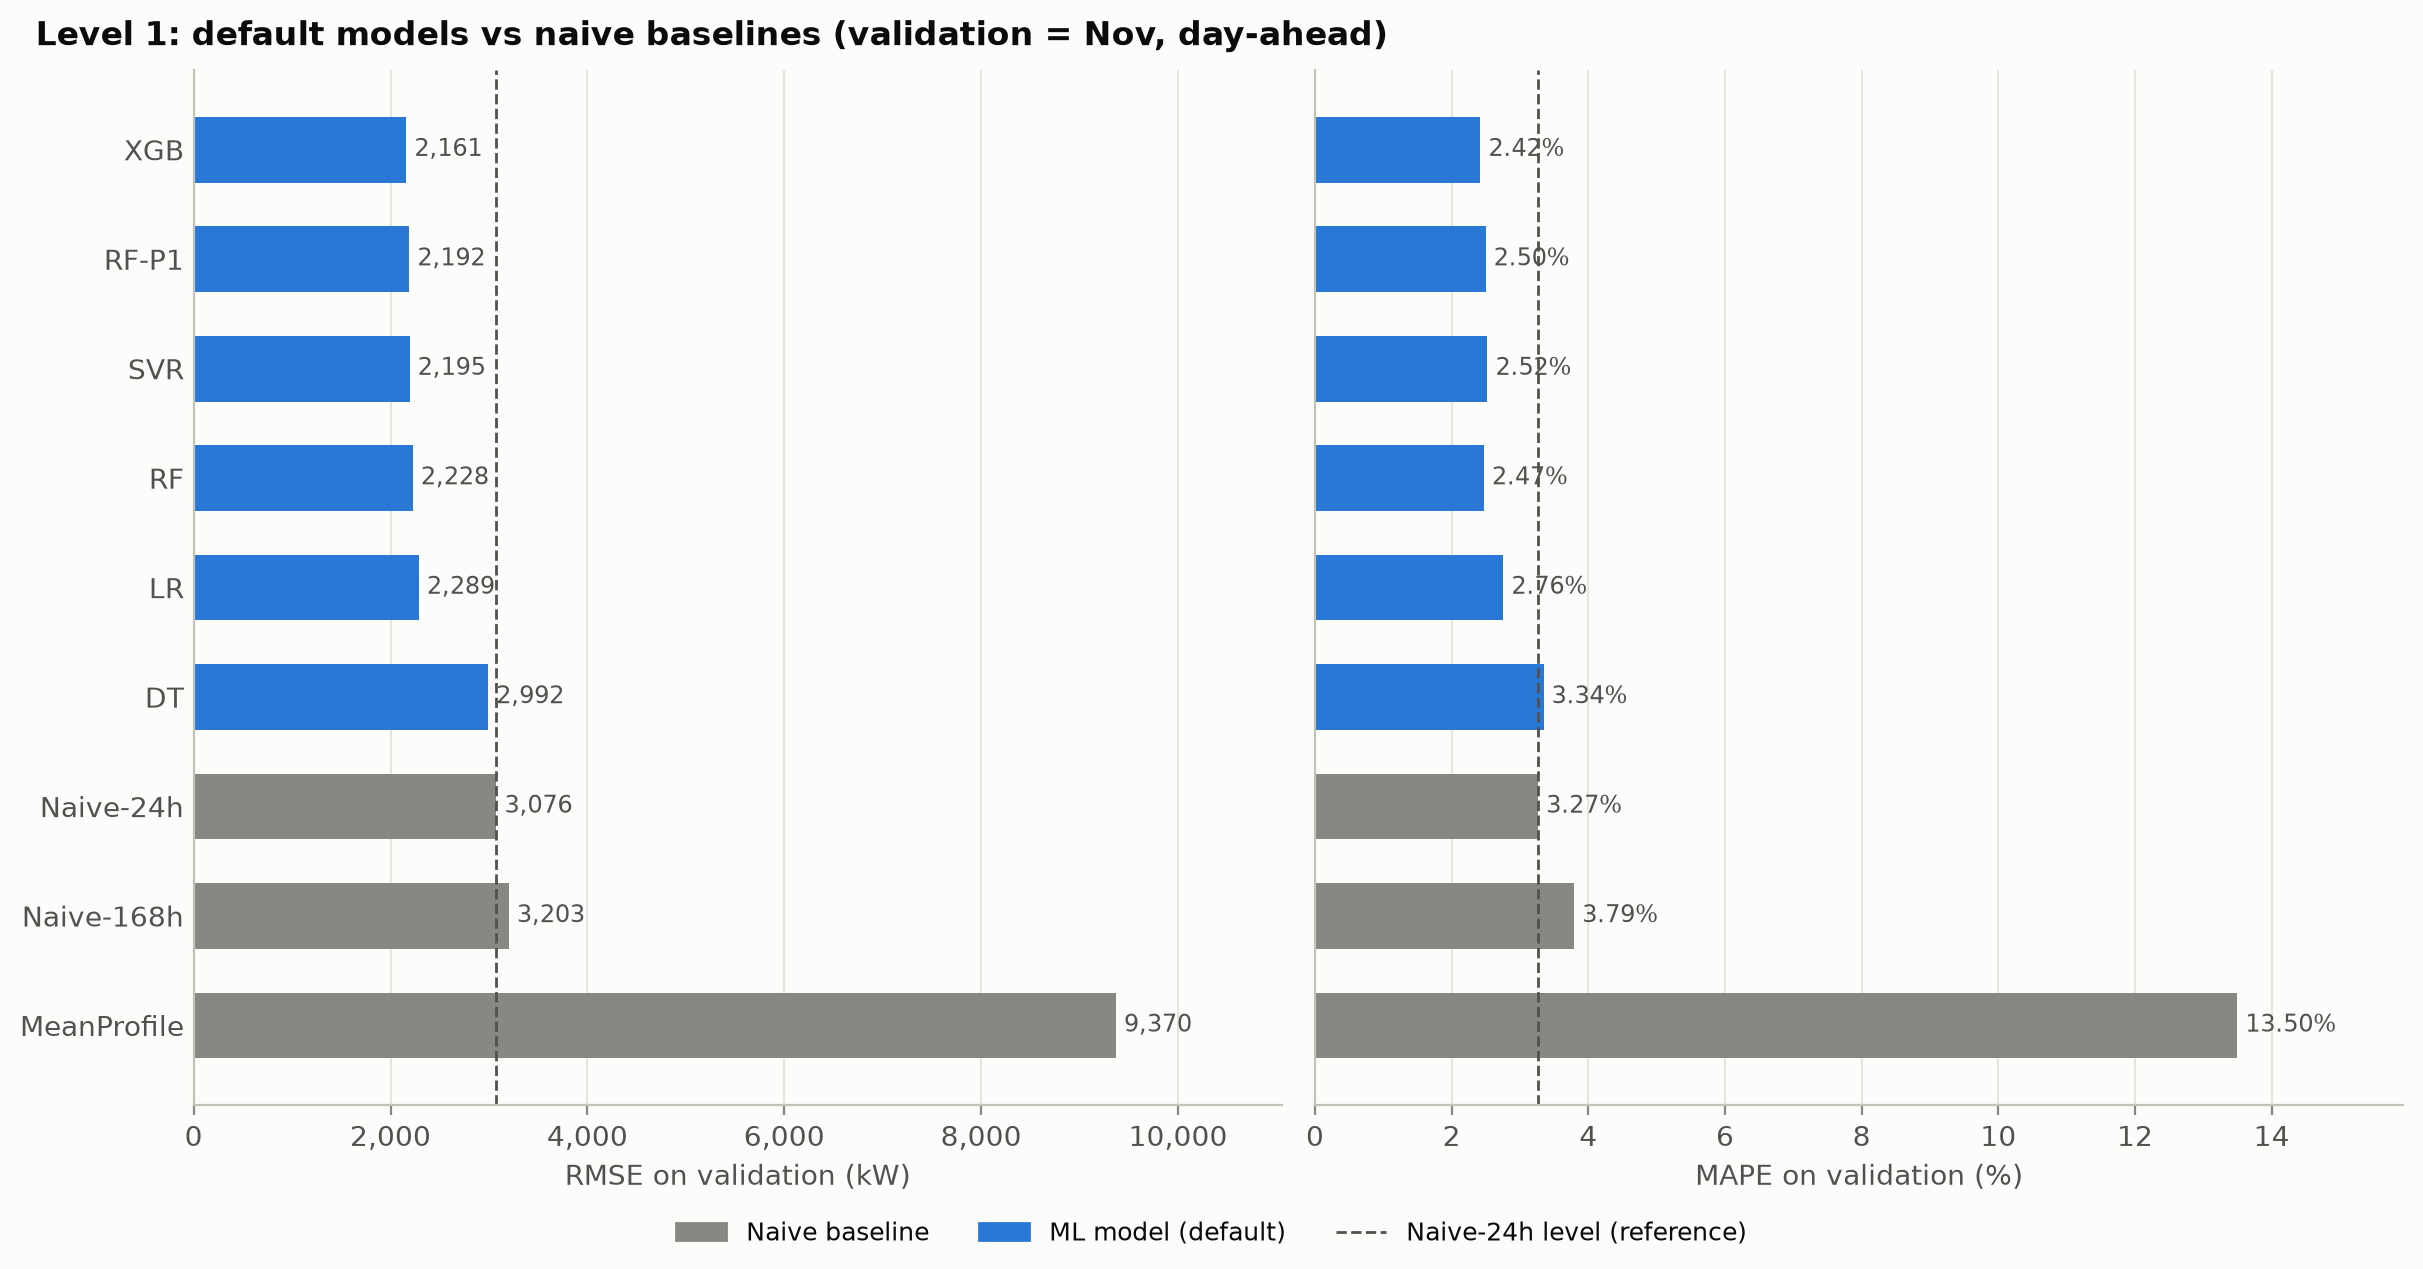
\includegraphics[width=\linewidth]{F11_level1_vs_baselines.png}
\caption{November h24 RMSE and MAPE for seasonal baselines, default regressors and RF-P1 (F11). The vertical references mark Naive-24h. Rankings and baseline improvements apply to this validation month.}\label{fig:baseline_comparison}
\end{figure}

The default decision tree illustrates why a statement that a model simply ``beats the baseline'' is incomplete. Its validation RMSE of \num{2992.4} kW improves on Naive-24h by \num{2.73}\%, but its MAE, \num{2190.0} kW, exceeds the baseline's \num{2080.7} kW. Its MAPE is also worse: \num{3.34}\% against \num{3.27}\%. Thus fewer or smaller large errors can coexist with worse average absolute error. This metric-specific interpretation follows the current CSV rather than earlier prose that labels DT uniformly unsuccessful.

Naive-168h reaches \num{3202.9} kW RMSE, slightly worse than Naive-24h. Weekly alignment alone therefore does not compensate for changes in the load level in this month. MeanProfile reaches \num{9369.6} kW RMSE. A training-wide calendar average cannot adapt its absolute level as directly as a recent measured load. This is consistent with the observed seasonal variation, although the comparison does not isolate a single cause of profile error.

\subsection{Training fit and representative validation behavior}
DT fits its training observations to numerical precision, yet its validation error remains substantial. RF and XGB have training RMSEs of \num{794.4} and \num{812.4} kW, well below their validation errors. These gaps indicate that training fit alone would give a misleading ranking. Conversely, LR has validation RMSE \num{2288.7} kW against training RMSE \num{2670.5} kW. A lower validation error is possible when the validation period is easier; it does not imply that model fitting used validation labels.

\Cref{fig:baseline_week} displays 13--19 November, the second Monday-to-Sunday week selected by the notebook. The previous-day baseline copies Sunday's lower daytime demand into Monday and carries Saturday's pattern into Sunday. XGB corrects much of these mismatches while retaining the broad daily trajectory. Calendar and history features provide a plausible explanation, but this plot alone cannot assign the improvement to a particular predictor. The civil holiday on 18 November offers only a single illustrative date, not an independent estimate of a general holiday effect.
\begin{figure}[tbp]\centering
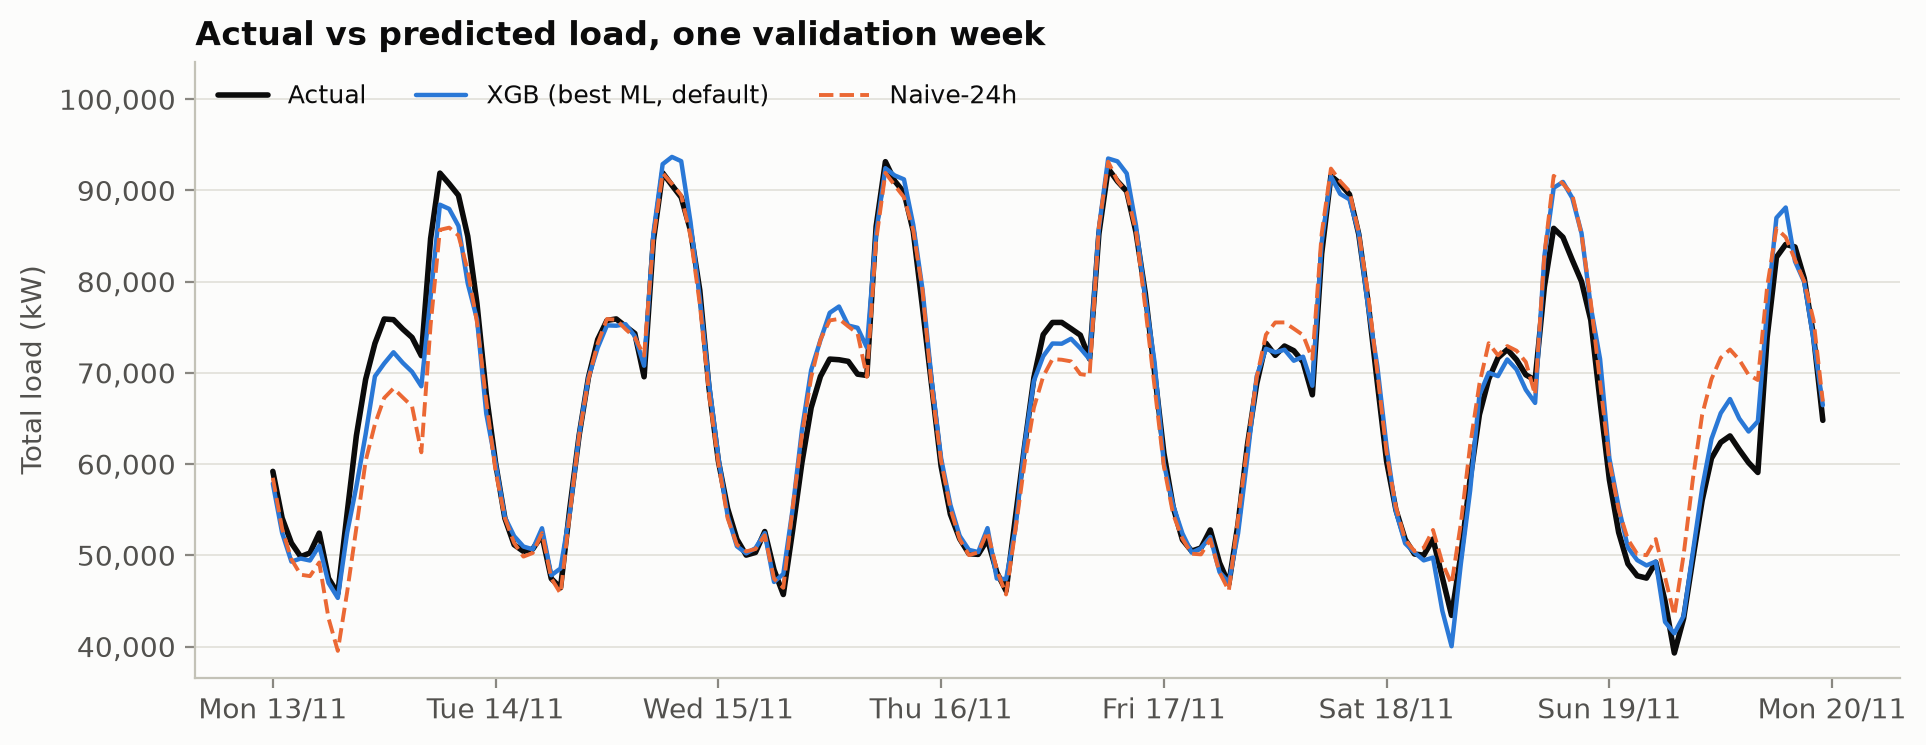
\includegraphics[width=\linewidth]{F11b_week_actual_vs_pred.png}
\caption{Actual load, default XGB forecasts and Naive-24h during 13--19 November (F11b). XGB was selected for this illustration by November validation RMSE. The week is part of model development and is not the December test.}\label{fig:baseline_week}
\end{figure}

The initial comparison supports proceeding to temporal validation: several regressors improve substantially on the seasonal baseline in November. It does not yet support selecting XGB for deployment, because a single autumn month omits the summer regime and provides no estimate of seasonal stability.
\evidence{Notebook 03 cells 6--19; \code{src/models.py}; \code{T04_level0_level1_wide.csv}; F11 and F11b. Numerical values refer to November validation unless explicitly identified as training metrics.}

\section{Time-Series Cross-Validation}\label{sec:cv}
\subsection{Protocol and aggregation}
Notebook 04 keeps the default estimators and h24 feature set D fixed while replacing the single November assessment with five expanding-window folds. This separates the effect of broader temporal evaluation from the parameter changes introduced later. Each validation window has 720 hours; training sizes increase from \num{4225} to \num{7105} hours. The exact dates appear in \cref{tab:folds}, and December is excluded. RF-P1 is not included in this stage's saved comparison.

For fold RMSEs $R_0,\ldots,R_4$, the reported summaries are
\begin{equation}
\overline R=\frac{1}{5}\sum_{k=0}^{4}R_k,\qquad
s_R=\sqrt{\frac{1}{4}\sum_{k=0}^{4}(R_k-\overline R)^2}.
\label{eq:cv_summary}
\end{equation}
The same mean/sample-SD convention applies to the other fold metrics. These are summaries of temporal variation under increasing training sizes. They are not confidence intervals, and the overlapping training windows do not constitute independent replications.

\subsection{Average performance and stability}
\Cref{tab:cv} changes the conclusion suggested by November alone. LR has the lowest default mean RMSE, \num{2792.3} kW, with SD \num{623.3} kW. RF and XGB follow at \num{3069.5} and \num{3264.8} kW, with much larger SDs of \num{1488.8} and \num{1815.8} kW. Naive-24h reaches \num{3392.4} kW with SD \num{421.5} kW. LR is the most stable default ML model by this dispersion measure, while Naive-24h has still lower dispersion overall.
\begin{table}[H]\centering\small
\caption{Default-model development CV, h24 (T05). SD is the sample standard deviation over five folds, not a confidence interval. Errors in kW; MAPE in percent.}\label{tab:cv}
\setlength{\tabcolsep}{4pt}
\begin{tabular}{lrrrr}
\toprule
Model & RMSE mean $\pm$ SD & MAE & MAPE & R$^2$ \\
\midrule
LR & \num{2792.3} $\pm$ \num{623.3} & \num{2101.0} & \num{2.95} & \num{0.9651} \\
RF & \num{3069.5} $\pm$ \num{1488.8} & \num{2168.6} & \num{2.82} & \num{0.9582} \\
XGB & \num{3264.8} $\pm$ \num{1815.8} & \num{2328.0} & \num{2.99} & \num{0.9510} \\
Naive-24h & \num{3392.4} $\pm$ \num{421.5} & \num{2371.7} & \num{3.28} & \num{0.9497} \\
SVR & \num{3968.7} $\pm$ \num{2891.5} & \num{2753.4} & \num{3.44} & \num{0.9224} \\
DT & \num{4048.2} $\pm$ \num{1410.4} & \num{2915.3} & \num{3.87} & \num{0.9294} \\
Naive-168h & \num{4892.6} $\pm$ \num{2297.1} & \num{3655.4} & \num{4.92} & \num{0.8887} \\
\bottomrule\end{tabular}
\end{table}


Default SVR and DT have mean RMSEs of \num{3968.7} and \num{4048.2} kW, exceeding Naive-24h. This does not contradict SVR's strong November result: November is only the final fold. Nor does LR's first-place RMSE ranking extend to every metric. RF has the lowest mean MAPE, \num{2.82}\%, compared with LR's \num{2.95}\%. The implemented selection objective remains mean RMSE rather than a retrospective choice of the most favorable metric; the repository does not establish prospective preregistration.

\Cref{tab:cv_folds,fig:cv_folds} expose the fold structure behind these averages. The last fold reproduces the November results for all eight shared models and baselines within the stored numerical tolerance. Among the five ML families, LR rises from fourth in November to first by mean CV RMSE; XGB moves from first to third and SVR from second to fourth. Across all eight entries, SVR is fifth because Naive-24h also ranks ahead of it. Stating the comparison population avoids confusing ML-only and combined rankings.
\begin{table}[tbp]\centering\small
\caption{Default h24 RMSE by temporal fold (T05), in kW. Models are ordered by mean fold RMSE; fold boundaries are given in Table~\ref{tab:folds}.}\label{tab:cv_folds}
\setlength{\tabcolsep}{4pt}
\begin{tabular}{lrrrrr}
\toprule
Model & Fold 0 & Fold 1 & Fold 2 & Fold 3 & Fold 4 \\
\midrule
LR & \num{3070.8} & \num{3307.8} & \num{3323.4} & \num{1970.8} & \num{2288.7} \\
RF & \num{5397.2} & \num{3456.3} & \num{2780.0} & \num{1486.8} & \num{2227.5} \\
XGB & \num{6229.6} & \num{3433.3} & \num{2988.7} & \num{1510.9} & \num{2161.4} \\
Naive-24h & \num{4024.4} & \num{3562.6} & \num{3328.4} & \num{2970.0} & \num{3076.4} \\
SVR & \num{8774.7} & \num{4352.6} & \num{3040.3} & \num{1480.6} & \num{2195.2} \\
DT & \num{6110.5} & \num{4663.4} & \num{3906.2} & \num{2568.3} & \num{2992.4} \\
Naive-168h & \num{6224.7} & \num{7205.0} & \num{6062.4} & \num{1768.2} & \num{3202.9} \\
MeanProfile & \num{21060.3} & \num{14973.6} & \num{6654.0} & \num{7967.9} & \num{9369.6} \\
\bottomrule\end{tabular}
\end{table}

\begin{figure}[tbp]\centering
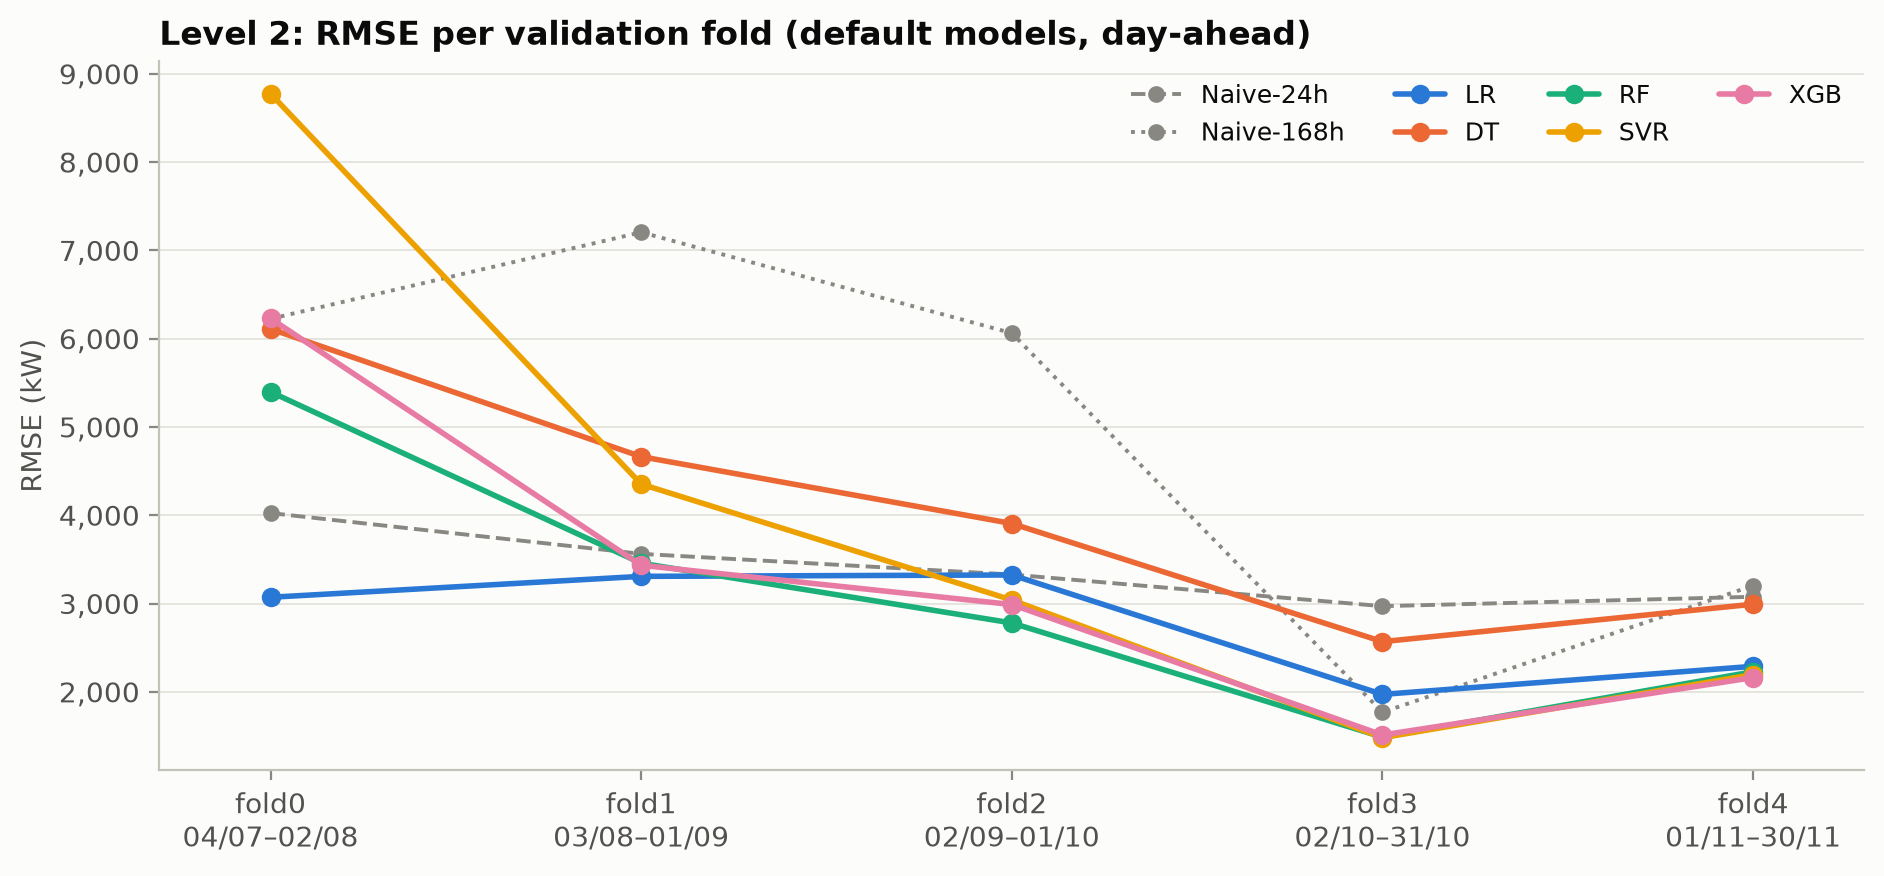
\includegraphics[width=\linewidth]{F12_rmse_per_fold.png}
\caption{Default h24 RMSE across expanding validation folds (F12). Fold 0 covers 4 July--2 August and reveals substantial sensitivity of several nonlinear estimators to the summer period. MeanProfile is omitted from the graphic but retained in the numerical tables.}\label{fig:cv_folds}
\end{figure}

\subsection{Summer distribution shift and model behavior}
The first fold is particularly difficult for default RF, XGB, SVR and DT, with RMSEs approximately \num{5397}, \num{6230}, \num{8775} and \num{6111} kW. LR and Naive-24h reach approximately \num{3071} and \num{4024} kW. The audit's hourly-data check finds that the largest training load is \num{110710.5} kW, while the largest validation load is \num{133129.8} kW; \num{12.22}\% of validation hours exceed the training maximum. This percentage is the fraction of observations above that maximum, not the percentage difference between the two maxima.

Standard regression-tree predictions are averages of training responses within leaves; an RF averages such predictions. Their absolute predictions therefore cannot exceed the training response range. This restriction makes unusually high validation loads challenging for those models. The same strict range bound does not apply generally to additive XGBoost or RBF SVR. Their summer errors are compatible with difficulty adapting to a shifted regime, but the saved experiments do not prove a unique failure mechanism for each estimator. The residual-target formulation in \cref{sec:tuning} tests a practical response to this difficulty.

Training and validation errors reinforce this qualification. The default tree interpolates training data, while RF and XGB have mean training RMSEs around \num{797.2} and \num{697.8} kW, far below their mean CV errors. Both overfitting and temporal distribution change can contribute to such gaps. A validation/training ratio cannot disentangle them by itself.

\subsection{Implications for subsequent selection}
The temporal folds demonstrate that November alone would favor a different default model. They also show that a recent-load baseline remains competitive when nonlinear defaults encounter a new regime. This motivates tuning regularization and comparing absolute with lag-relative targets using the common folds. However, these same development folds have already informed feature and modeling decisions. Their later reuse in search introduces selection uncertainty that fold SD does not quantify. The separate December evaluation must retain the CV selection rule and cannot convert these development scores into unbiased estimates of future performance.
\evidence{Notebook 04 cells 6--19; \code{T05_level2_cv.csv}; \code{T05_level2_summary.csv}; \code{T02_cv_folds.csv}; F12; \code{report/evidence/numerical_checks.json} for the fraction above the fold-0 training maximum.}

\section{Hyperparameter Optimization}\label{sec:tuning}
\subsection{Search design and optimization objective}
Notebook 05 applies \code{RandomizedSearchCV} to five model families, each with absolute and lag-relative targets. Random search allocates a finite budget across joint parameter configurations rather than enumerating a Cartesian grid\cite{bergstra2012}. Each configuration is evaluated on the same five expanding development folds with RMSE, MAE, MAPE and R$^2$ scorers. The selected configuration minimizes mean fold RMSE:
\begin{equation}
\theta^*_{m,q}=\underset{\theta\in\mathcal S_{m,q}}{\operatorname{arg\,min}}\;
\frac{1}{5}\sum_{k=0}^{4}\mathrm{RMSE}_{k}(m,q,\theta),
\label{eq:search_objective}
\end{equation}
where $m$ is the family, $q$ the target formulation, and $\mathcal S_{m,q}$ the sampled configurations. The implementation retrieves the smallest \code{rank_test_RMSE}; it does not select by MAE or MAPE. Negative sklearn error scores are converted back to positive errors for reporting.

Searches use seed 42 and \code{refit=False}. Thus the search stage stores results and chosen parameters without fitting a final estimator on the entire development set. Final refitting belongs to notebook 07. Outer search parallelism follows \code{TETOUAN_N_JOBS}, while inner estimators are configured with one job where supported. No Bayesian optimization, grid-search refinement or early-stopping stage is implemented.

\Cref{tab:search_space} records the actual distributions and discrete choices. LR has 20 candidates per formulation, DT 40, RF 30, SVR 30 and XGB 50. With two formulations, this gives 340 sampled configurations and \num{1700} CV fits for h24. The independent h1 searches add the same budget, giving \num{3400} fits across both horizons, excluding baselines, ablations and subsequent refits. These counts describe the saved experiment design; no searches were rerun for this report.
\begingroup\small\setlength{\tabcolsep}{4pt}
\begin{longtable}{p{.10\linewidth}p{.24\linewidth}p{.48\linewidth}r}
\caption{Search spaces shared by both horizons and both target formulations (T06). Budgets are per model formulation, not per parameter. Integer limits are inclusive as displayed.}\label{tab:search_space}\\
\toprule
Model & Parameter & Distribution / values & Budget \\
\midrule\endfirsthead
\multicolumn{4}{l}{\small\itshape Continued from previous page}\\\toprule
Model & Parameter & Distribution / values & Budget \\
\midrule\endhead\bottomrule\endfoot
LR & alpha & log-uniform(0.001, 1000.0) & \num{20} \\
DT & max\_depth & 4, 6, 8, 10, 15, 20, None & \num{40} \\
DT & min\_samples\_leaf & 1, 5, 10, 20, 50 & \num{40} \\
DT & min\_samples\_split & 2, 10, 20, 50 & \num{40} \\
DT & max\_features & None, sqrt, 0.5, 0.8 & \num{40} \\
RF & n\_estimators & 100, 200, 300, 500 & \num{30} \\
RF & max\_depth & 10, 20, 30, None & \num{30} \\
RF & min\_samples\_leaf & 1, 2, 5, 10 & \num{30} \\
RF & max\_features & sqrt, 0.3, 0.5, 0.8, 1.0 & \num{30} \\
SVR & C & log-uniform(0.1, 1000.0) & \num{30} \\
SVR & gamma & log-uniform(0.0001, 1) & \num{30} \\
SVR & epsilon & 0.01, 0.05, 0.1, 0.2 & \num{30} \\
XGB & n\_estimators & integer 200 ... 1499 & \num{50} \\
XGB & learning\_rate & log-uniform(0.01, 0.2) & \num{50} \\
XGB & max\_depth & integer 3 ... 10 & \num{50} \\
XGB & subsample & uniform(0.6, 1.0) & \num{50} \\
XGB & colsample\_bytree & uniform(0.6, 1.0) & \num{50} \\
XGB & min\_child\_weight & integer 1 ... 10 & \num{50} \\
XGB & reg\_lambda & log-uniform(0.1, 10.0) & \num{50} \\
\end{longtable}\endgroup


The tuned LR implementation is Ridge, whereas the default LR is ordinary least squares. Accordingly, its comparison includes a change in regularization family. SVR standardizes both predictors and the response inside training-fitted wrappers, so its $C$ and $\epsilon$ are interpreted on the standardized target scale. Integer endpoints in \cref{tab:search_space} reflect the exclusive upper limits in the Python distributions. For example, the XGB tree-count support is 200--1499.

\subsection{Absolute and residual formulations}
For h24, the residual version learns $r_t=y_t-y_{t-24}$ and returns $y_{t-24}+\widehat r_t$, as defined in \cref{eq:delta}. The available lag remains among the inputs. This allows the known recent level to be carried directly into a prediction, leaving the estimator to model a correction. It can help an absolute tree model facing levels outside its fitted response range, but it does not ensure that future corrections are represented in training.

Absolute and residual searches use the same parameter distributions, budgets and random seed, and therefore sample matching underlying configurations within a family. Each formulation selects its own minimum-RMSE candidate. Consequently, a residual-versus-absolute comparison includes any change in the selected parameters as well as the change in response formulation. It is not a fixed-parameter causal estimate of the target transformation alone.

\subsection{Selected configurations and development results}
\Cref{tab:selected_h24} gives all ten selected h24 configurations, generated from the saved JSON. For the ultimately selected absolute SVR, $C=\num{26.926469}$, $\epsilon=\num{0.01}$ and $\gamma=\num{0.006339}$ after rounding. The JSON retains full precision. The absolute DT selects depth eight, while its residual version selects depth four. The residual RF uses 100 trees, minimum leaf size ten and square-root feature sampling; its absolute counterpart uses 200 trees, minimum leaf size two and a feature fraction of 0.8. These examples show that the best configurations depend on the response formulation.
\begingroup\small\setlength{\tabcolsep}{4pt}
\begin{longtable}{p{.16\linewidth}p{.76\linewidth}}
\caption{Selected h24 hyperparameters from best\_params.json. Estimator-wrapper prefixes are omitted; floating values are rounded to six decimals. Both target formulations were searched independently.}\label{tab:selected_h24}\\
\toprule
Variant & Selected parameters \\
\midrule\endfirsthead
\multicolumn{2}{l}{\small\itshape Continued from previous page}\\\toprule
Variant & Selected parameters \\
\midrule\endhead\bottomrule\endfoot
LR & alpha = \num{0.001329} \\
LR $\Delta$ & alpha = \num{98.777003} \\
DT & min\_samples\_split = 10; min\_samples\_leaf = 5; max\_features = None; max\_depth = 8 \\
DT $\Delta$ & min\_samples\_split = 20; min\_samples\_leaf = 5; max\_features = None; max\_depth = 4 \\
RF & n\_estimators = 200; min\_samples\_leaf = 2; max\_features = \num{0.800000}; max\_depth = 30 \\
RF $\Delta$ & n\_estimators = 100; min\_samples\_leaf = 10; max\_features = sqrt; max\_depth = 30 \\
SVR & C = \num{26.926469}; epsilon = \num{0.010000}; gamma = \num{0.006339} \\
SVR $\Delta$ & C = \num{138.262322}; epsilon = \num{0.100000}; gamma = \num{0.003387} \\
XGB & colsample\_bytree = \num{0.798899}; learning\_rate = \num{0.024629}; max\_depth = 3; min\_child\_weight = 8; n\_estimators = 1304; reg\_lambda = \num{0.341635}; subsample = \num{0.990646} \\
XGB $\Delta$ & colsample\_bytree = \num{0.831312}; learning\_rate = \num{0.011137}; max\_depth = 3; min\_child\_weight = 10; n\_estimators = 774; reg\_lambda = \num{9.197754}; subsample = \num{0.935573} \\
\end{longtable}\endgroup


\Cref{tab:tuning,fig:tuning} compares these candidates with each family's absolute default. Define the displayed improvement as
\begin{equation}
G_{m,q}=100\left(1-\frac{\overline R_{m,q,\mathrm{tuned}}}{\overline R_{m,\mathrm{default}}}\right).
\label{eq:tuning_gain}
\end{equation}
For residual rows, $G_{m,q}$ combines parameter selection with a target change. The tuned absolute SVR has the lowest mean CV RMSE, \num{2410.6} kW with sample SD \num{766.3} kW, a \num{39.26}\% reduction from its default. Its residual counterpart follows at \num{2427.1} kW. RF residual and XGB residual reach \num{2429.3} and \num{2441.0} kW. The four leading means span only \num{30.4} kW, or \num{1.26}\% of the best mean, which is small relative to their temporal SDs. This does not establish equivalence or statistical significance.
\begin{table}[H]\centering\small
\caption{Tuned h24 development CV (T07). RMSE and its SD are in kW. Improvement compares each row with the absolute default model of that family; $\Delta$ rows combine tuning with a target change.}\label{tab:tuning}
\setlength{\tabcolsep}{4pt}
\begin{tabular}{lrrrr}
\toprule
Variant & Default RMSE & Tuned RMSE $\pm$ SD & Gain (\%) & MAPE (\%) \\
\midrule
SVR & \num{3968.7} & \num{2410.6} $\pm$ \num{766.3} & \num{39.26} & \num{2.42} \\
SVR $\Delta$ & \num{3968.7} & \num{2427.1} $\pm$ \num{773.7} & \num{38.84} & \num{2.41} \\
RF $\Delta$ & \num{3069.5} & \num{2429.3} $\pm$ \num{800.7} & \num{20.86} & \num{2.36} \\
XGB $\Delta$ & \num{3264.8} & \num{2441.0} $\pm$ \num{785.5} & \num{25.23} & \num{2.38} \\
DT $\Delta$ & \num{4048.2} & \num{2524.9} $\pm$ \num{851.9} & \num{37.63} & \num{2.40} \\
LR $\Delta$ & \num{2792.3} & \num{2770.0} $\pm$ \num{591.6} & \num{0.80} & \num{2.87} \\
LR & \num{2792.3} & \num{2792.3} $\pm$ \num{623.3} & \num{0.00} & \num{2.95} \\
XGB & \num{3264.8} & \num{3009.9} $\pm$ \num{1470.2} & \num{7.81} & \num{2.80} \\
RF & \num{3069.5} & \num{3010.4} $\pm$ \num{1588.7} & \num{1.93} & \num{2.75} \\
DT & \num{4048.2} & \num{3589.7} $\pm$ \num{1756.1} & \num{11.33} & \num{3.34} \\
\bottomrule\end{tabular}
\end{table}

\begin{figure}[tbp]\centering
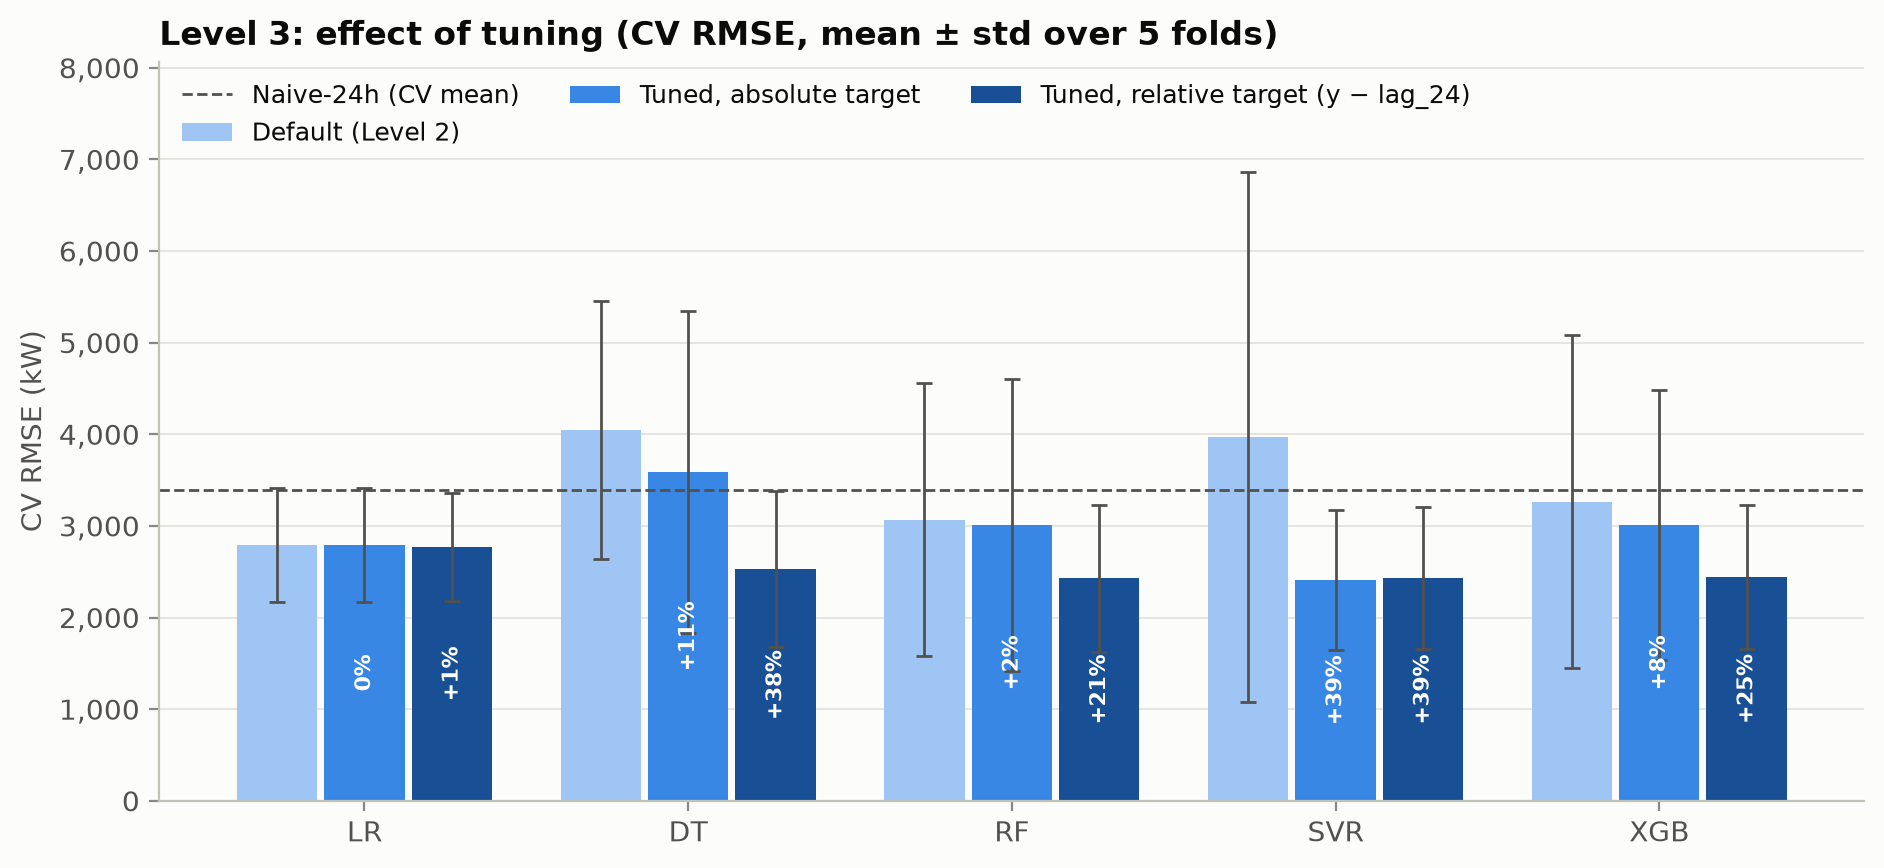
\includegraphics[width=\linewidth]{F13_default_vs_tuned.png}
\caption{Default, tuned absolute and tuned residual h24 CV RMSE by model family (F13). Error bars are sample SDs over five temporal folds. Bar percentages compare against the absolute default, so residual improvements include both tuning and target reformulation.}\label{fig:tuning}
\end{figure}

Within the tuned comparisons, residual targets improve mean RMSE for LR, DT, RF and XGB; absolute SVR remains slightly better than residual SVR. RF residual also has the lowest displayed mean MAPE, \num{2.36}\%, whereas absolute SVR has \num{2.42}\%. Model selection nevertheless follows mean RMSE. Absolute DT still exceeds Naive-24h in mean CV RMSE, \num{3589.7} against \num{3392.4} kW. Thus tuning does not make every individual variant superior to the baseline. The absolute Ridge result is effectively unchanged from default OLS; its tiny numerical deterioration is not a meaningful improvement.

\subsection{Search interpretation and selection boundary}
All ten h24 search CSVs and ten h1 counterparts were checked in the prior audit for candidate counts, selected rows, parameters and fold metrics. The searches support comparison within their sampled budgets; they do not establish global optima. F14, the saved five-panel search diagnostic, varies multiple parameters across its plotted configurations. Its apparent associations with a single horizontal-axis parameter therefore cannot be interpreted as controlled sensitivity effects.

The same folds are used both to choose parameters and to report the selected CV means. Feature and target choices also reuse development data. No nested assessment or repeated-seed search is stored, so the magnitude of selection bias remains unquantified. The model identity passed to final h24 analysis is the absolute SVR because it minimizes development mean RMSE. A lower December error from a different variant must remain a test observation, rather than a reason to revise this selection retrospectively.
\evidence{Notebook 05 cells 4--23; \code{src/models.py::search_spaces}; T06/T07; \code{best_params.json}; ten h24 \code{search_*.csv} files. Notebook 06 supplies the ten separate h1 searches; selected configurations and fold scores were checked in the completed audit.}

\section{Ablation Studies and Forecast-Horizon Analysis}\label{sec:ablation}
\subsection{Feature-set design and comparison limits}
Notebook 06 examines feature groups with RF and XGB, each using absolute and residual targets where the residual base exists. It evaluates the same eligible h24 timestamps and the same five temporal folds as the preceding stages. Parameters are frozen at the values selected on set D; they are not retuned for every feature subset. The results therefore assess feature changes under D-selected configurations, rather than the best attainable performance of each subset.

Sets A--E add groups cumulatively: A contains the five weather variables; B adds seven calendar variables; C adds three special-day indicators; D adds daily lags 24 and 48; E adds lag 168, the 24-hour rolling mean and SD, and the 168-hour rolling mean. Their sizes are 5, 12, 15, 17 and 21. F removes the five weather variables from E, leaving 16. In particular, F is not D without weather. Residual models are evaluated only on D--F because A--C omit their lag-24 base.

For successive evaluated sets $U,V$, the reported relative RMSE change is
\begin{equation}
\delta_{U\rightarrow V}=100\left(\frac{\overline R_V}{\overline R_U}-1\right).
\label{eq:ablation_change}
\end{equation}
Negative values indicate improvement. Each comparison is conditional on the included groups and fixed parameters; predictive ablation does not identify causal effects of weather, holidays or consumption history.

\subsection{Daily history dominates the tested feature additions}
\Cref{tab:ablation,fig:ablation} show substantial error reduction when calendar variables supplement weather. Nevertheless, weather, calendar and special days alone remain much worse than Naive-24h. Adding daily lags from C to D lowers absolute RF mean RMSE from \num{9168.1} to \num{3010.4} kW, a \num{67.16}\% reduction. For absolute XGB, the corresponding change is \num{8740.2} to \num{3009.9} kW, or \num{65.56}\%. These are the largest relative reductions among the sequential additions tested here.
\begin{table}[tbp]\centering\small
\caption{Feature ablation with fixed D-selected hyperparameters: mean CV RMSE in kW (T09). Missing entries were not run because the residual base is absent.}\label{tab:ablation}
\setlength{\tabcolsep}{4pt}
\begin{tabular}{lrrrr}
\toprule
Set (columns) & RF & XGB & RF $\Delta$ & XGB $\Delta$ \\
\midrule
A (5) & \num{15010.3} & \num{14826.7} & -- & -- \\
B (12) & \num{10040.9} & \num{9669.3} & -- & -- \\
C (15) & \num{9168.1} & \num{8740.2} & -- & -- \\
D (17) & \num{3010.4} & \num{3009.9} & \num{2429.3} & \num{2441.0} \\
E (21) & \num{3700.3} & \num{4921.4} & \num{2741.8} & \num{3964.2} \\
F (16) & \num{3759.2} & \num{5017.1} & \num{2887.5} & \num{3928.4} \\
\bottomrule\end{tabular}
\end{table}

\begin{figure}[tbp]\centering
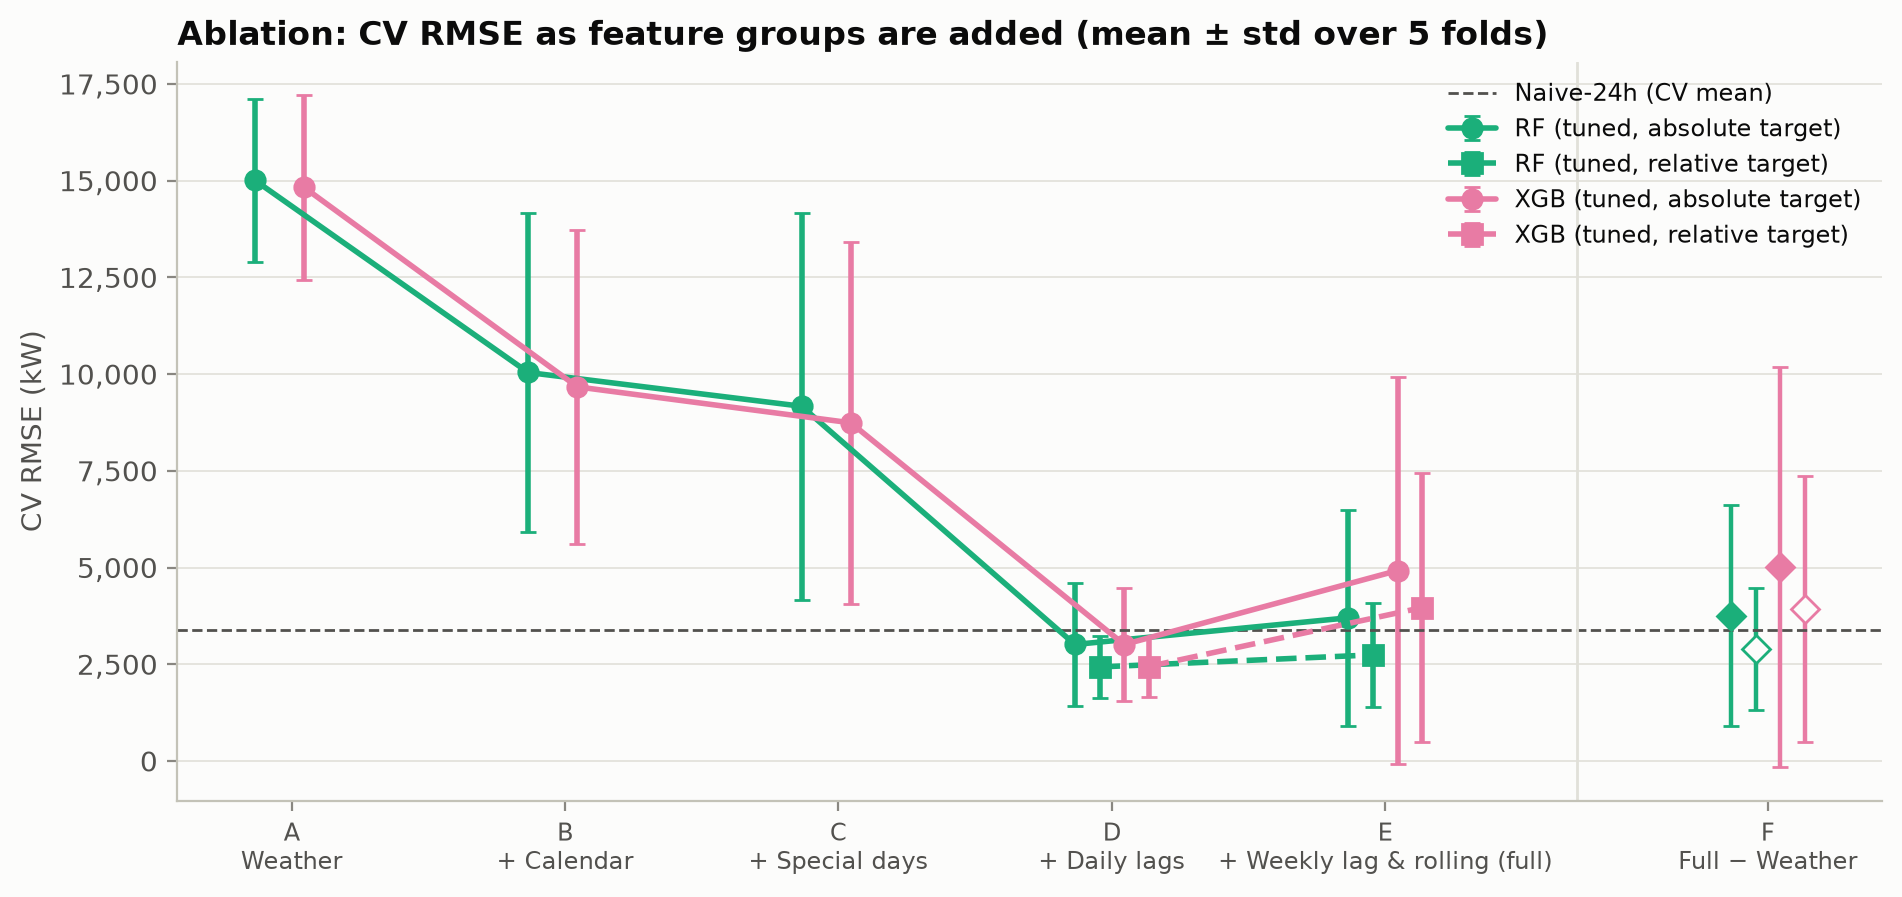
\includegraphics[width=\linewidth]{F15_ablation.png}
\caption{RF/XGB h24 feature ablation with D-selected hyperparameters held fixed (F15). Error bars show fold sample SD. Residual models begin at D because they require lag-24; F removes weather from E. These are conditional predictive comparisons.}\label{fig:ablation}
\end{figure}

The daily histories provide a recent load level that weather and fixed calendar indicators do not fully capture. This interpretation agrees with the seasonal naive results, but the experiment cannot separate the individual contributions of lag 24 and lag 48 because they are added together. On D, residual RF and residual XGB improve further to \num{2429.3} and \num{2441.0} kW, respectively. Residual RF on D has the lowest mean RMSE among the configurations included in this ablation.

\subsection{Weekly, rolling and weather comparisons}
Adding weekly and rolling predictors from D to E worsens mean RMSE for all four variants. Absolute RF increases by \num{22.92}\% and absolute XGB by \num{63.51}\%; residual RF and residual XGB increase by \num{12.86}\% and \num{62.40}\%. More historical summaries therefore do not guarantee improvement under the selected configurations. Redundant predictors, regime-dependent relationships and parameter interactions are possible explanations, but no experiment isolates their respective roles. In particular, the disadvantage of E may partly reflect choosing parameters on D.

Weather removal from E to F increases RMSE by \num{1.59}\% for absolute RF, \num{1.95}\% for absolute XGB and \num{5.31}\% for residual RF. Residual XGB instead improves by \num{0.90}\%. Thus the measured weather contribution is not uniformly positive, and its magnitude depends on the fitted formulation and other predictors. This comparison does not quantify the operational penalty of replacing observed weather with forecasts: it uses no forecast-error archive, omits a D-without-weather comparison, and does not evaluate the selected SVR. It cannot establish that oracle-weather optimism is negligible for the final model.

\subsection{Separately tuned hourly setting}
The h1 experiment uses 19 inputs: the same weather, calendar and special-day groups, plus lags 1, 2, 3 and 24. Its residual base is lag 1. It repeats the ten model/formulation searches using the same distributions, budgets and temporal validation dates, rather than transferring h24 parameters without tuning. h1 has 23 additional early-January training hours because of its different warm-up. Validation observations are identical across the two settings.

\Cref{tab:horizon,fig:horizon} compares each family's better formulation by development mean RMSE. LR, DT, RF and XGB use residual formulations in both settings; SVR uses absolute targets. Absolute SVR has h1 mean CV RMSE \num{1866.4} kW and MAPE \num{1.86}\%, compared with h24 values \num{2410.6} kW and \num{2.42}\%. Its RMSE is \num{22.57}\% lower in h1. All five family representatives have lower mean RMSE in h1, but the effect is heterogeneous: DT changes only from \num{2524.9} to \num{2489.6} kW, while XGB changes from \num{2441.0} to \num{2111.7} kW.
\begin{table}[tbp]\centering\small
\caption{Development CV horizon comparison (T10), RMSE in kW: best formulation within each family chosen separately per horizon. LR, DT, RF and XGB use residual targets; SVR uses the absolute target.}\label{tab:horizon}
\setlength{\tabcolsep}{4pt}
\begin{tabular}{lrrrr}
\toprule
Model & h24 RMSE & h1 RMSE & h24 MAPE (\%) & h1 MAPE (\%) \\
\midrule
Persistence & -- & \num{6332.9} & -- & \num{6.40} \\
Naive-24h & \num{3392.4} & \num{3392.4} & \num{3.28} & \num{3.28} \\
Naive-168h & \num{4892.6} & \num{4892.6} & \num{4.92} & \num{4.92} \\
MeanProfile & \num{12005.1} & \num{11997.4} & \num{13.83} & \num{13.82} \\
LR & \num{2770.0} & \num{2420.5} & \num{2.87} & \num{2.50} \\
DT & \num{2524.9} & \num{2489.6} & \num{2.40} & \num{2.29} \\
RF & \num{2429.3} & \num{2183.5} & \num{2.36} & \num{2.05} \\
SVR & \num{2410.6} & \num{1866.4} & \num{2.42} & \num{1.86} \\
XGB & \num{2441.0} & \num{2111.7} & \num{2.38} & \num{1.98} \\
\bottomrule\end{tabular}
\end{table}

\begin{figure}[tbp]\centering
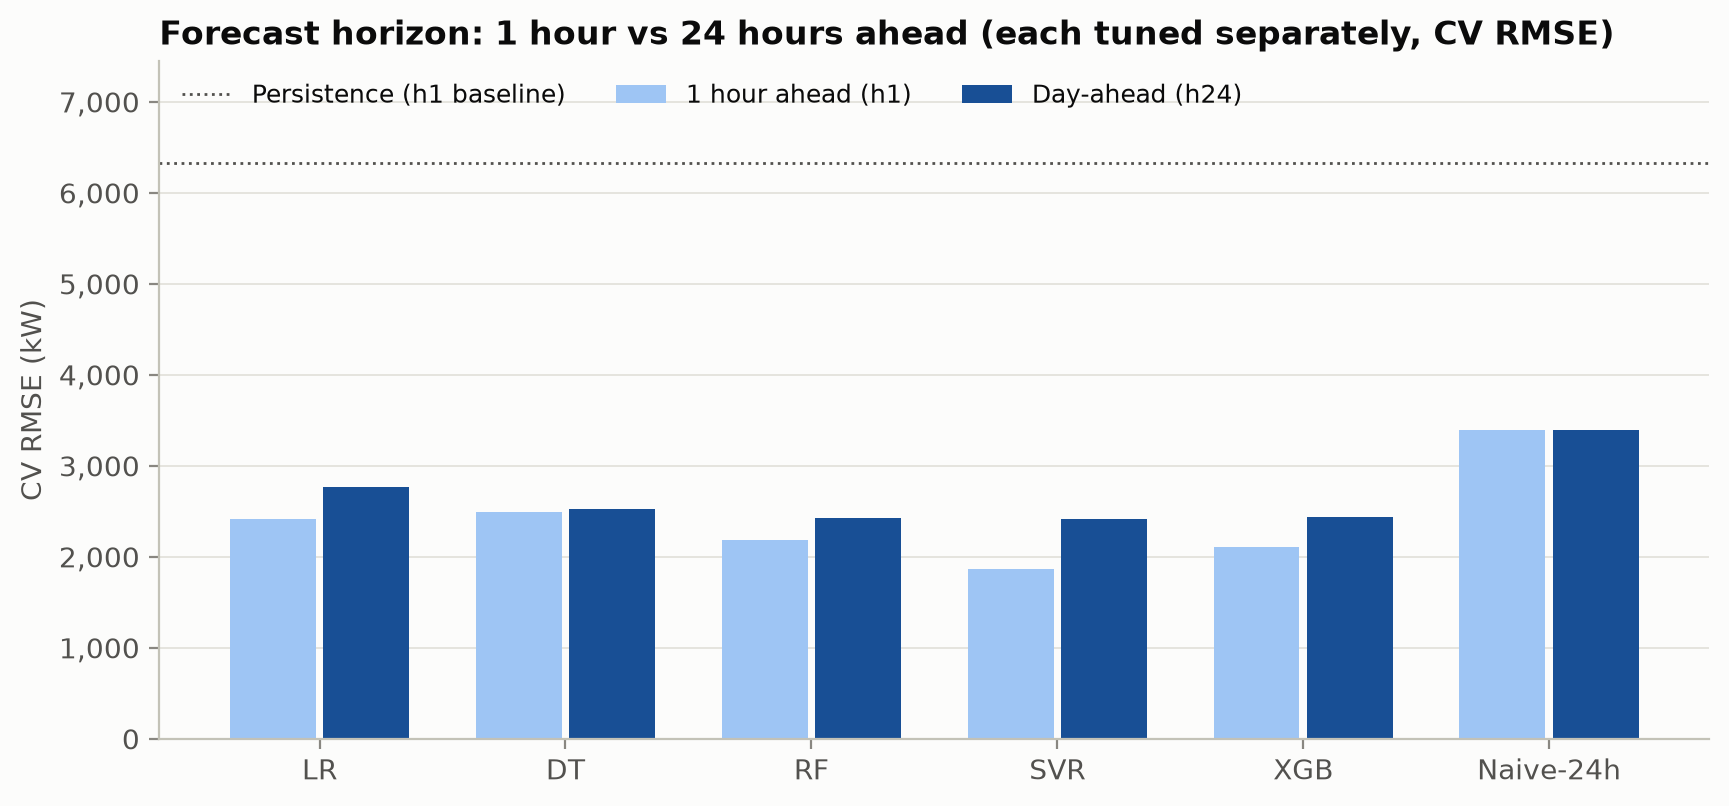
\includegraphics[width=\linewidth]{F15b_horizon.png}
\caption{Development CV RMSE for separately tuned h24 and h1 family representatives (F15b). Each bar uses the better target formulation within its family and setting. The h24 label denotes the daily-batch/minimum-lag convention explained in \cref{sec:features}, rather than a uniform 24-hour issuance lead.}\label{fig:horizon}
\end{figure}

The h1 persistence baseline has mean RMSE \num{6332.9} kW, substantially worse than Naive-24h at \num{3392.4} kW. A recent observation alone can be inaccurate when the demand curve changes rapidly between consecutive hours; the result demonstrates that shorter lag is not automatically a better naive forecast. A trained model can combine recent and seasonal history with calendar information rather than simply copying the previous hour.

Absolute SVR remains the lowest-mean-RMSE candidate among all stored h1 variants. Residual SVR is close at \num{1874.1} kW, and the h1 LR residual advantage over absolute Ridge is only about \num{0.0005} kW. Such a numerical difference should not be interpreted as a practically meaningful gain. The selected absolute SVR parameters happen to match across horizons, despite the searches being conducted separately.

\subsection{Scope of the horizon conclusion}
These results compare two implemented forecasting configurations. Alongside the history cutoff, they change the selected history columns, residual base, optimized parameters and early training sample count. Both retain observed target-hour weather. Consequently, the contrast supports an empirical advantage for the h1 configuration under this protocol, rather than a controlled universal law relating error to forecast lead. It also remains development evidence: the December evaluation must use the CV-selected absolute SVR for each setting and report test rankings separately.
\evidence{Notebook 06 cells 4--19; \code{T09_ablation_summary.csv}; \code{T10_horizon.csv}; \code{T10_horizon_cv.csv}; \code{best_params_h1.json}; ten \code{search_h1_*.csv} files; F15 and F15b. Feature membership is defined in \code{src/features.py}.}

\section{Final Test Evaluation and Error Analysis}\label{sec:final}
\subsection{Chronological test protocol and selection rule}
Notebook 07 refits the h24 estimators on all \num{7825} eligible development hours through 30 November and evaluates 720 hours from 1--30 December. The h1 development set contains \num{7848} hours and uses the same December timestamps. Model weights remain fixed during each evaluation, while historical-load predictors update with measurements from completed hours or days. These are updating forecasts, not an open-loop prediction of December from a single November cutoff. Observed target-hour weather remains an oracle input.

The final identity follows minimum development mean CV RMSE: absolute-target SVR for both settings. For h24, the notebook evaluates all default, tuned absolute and tuned residual variants; for h1, it evaluates each family's CV-preferred tuned formulation. The h1 table therefore contains fewer ML variants and does not establish a December ranking of all ten searched h1 formulations.

December is held outside the training and model-selection folds, but the repository does not establish a strictly single-use test. Whole-year descriptive EDA includes it, and the progress documentation records repeated final evaluation for reproducibility checks. The notebook's selection expression reads CV scores, even though it appears after calculation of the test table. This supports a CV-based selection rule, rather than prospective proof that every human modeling decision preceded all exposure to December.

\subsection{h24 performance and the residual-SVR result}
\Cref{tab:test24} reports the complete saved h24 comparison. The selected SVR achieves RMSE \num{1624.6} kW, MAE \num{1094.6} kW, MAPE \num{1.78}\% and R$^2=\num{0.9869}$. Against Naive-24h at \num{3296.3} kW RMSE, the reduction is \num{50.71}\%. Naive-168h is stronger than Naive-24h in December, with RMSE \num{2619.8} kW, but remains worse than the selected SVR. Thus the model improves on both seasonal reference rules in this period.
\begin{table}[H]\centering\small
\caption{December test, h24 (T08), ordered by test RMSE. The model chosen on CV before the test is SVR-tuned. RMSE/MAE in kW; skill is the RMSE reduction against Naive-24h.}\label{tab:test24}
\setlength{\tabcolsep}{4pt}
\begin{tabular}{lrrrrr}
\toprule
Model & RMSE & MAE & MAPE (\%) & R$^2$ & Skill (\%) \\
\midrule
SVR $\Delta$-tuned & \num{1419.1} & \num{1046.1} & \num{1.72} & \num{0.9900} & \num{56.95} \\
SVR-tuned & \num{1624.6} & \num{1094.6} & \num{1.78} & \num{0.9869} & \num{50.71} \\
XGB-tuned & \num{1711.5} & \num{1233.5} & \num{2.03} & \num{0.9854} & \num{48.08} \\
XGB $\Delta$-tuned & \num{1719.2} & \num{1209.9} & \num{2.00} & \num{0.9853} & \num{47.84} \\
RF $\Delta$-tuned & \num{1761.9} & \num{1171.4} & \num{1.93} & \num{0.9846} & \num{46.55} \\
XGB-default & \num{1891.0} & \num{1330.3} & \num{2.15} & \num{0.9822} & \num{42.63} \\
DT $\Delta$-tuned & \num{2005.2} & \num{1316.7} & \num{2.20} & \num{0.9800} & \num{39.17} \\
RF-tuned & \num{2017.1} & \num{1331.7} & \num{2.19} & \num{0.9798} & \num{38.81} \\
RF-default & \num{2044.3} & \num{1360.8} & \num{2.24} & \num{0.9792} & \num{37.98} \\
SVR-default & \num{2063.7} & \num{1300.5} & \num{2.20} & \num{0.9788} & \num{37.39} \\
LR-tuned & \num{2169.6} & \num{1624.8} & \num{2.74} & \num{0.9766} & \num{34.18} \\
LR-default & \num{2169.6} & \num{1624.8} & \num{2.74} & \num{0.9766} & \num{34.18} \\
LR $\Delta$-tuned & \num{2217.3} & \num{1629.1} & \num{2.74} & \num{0.9755} & \num{32.73} \\
Naive-168h & \num{2619.8} & \num{1775.4} & \num{2.87} & \num{0.9658} & \num{20.52} \\
DT-tuned & \num{2846.6} & \num{1960.3} & \num{3.19} & \num{0.9597} & \num{13.64} \\
DT-default & \num{2989.6} & \num{1987.4} & \num{3.28} & \num{0.9555} & \num{9.30} \\
Naive-24h & \num{3296.3} & \num{2071.5} & \num{3.39} & \num{0.9459} & \num{0.00} \\
\bottomrule\end{tabular}
\end{table}


Residual SVR has the lowest observed test RMSE, \num{1419.1} kW, with MAE \num{1046.1} kW, MAPE \num{1.72}\% and R$^2=\num{0.9900}$. It was slightly worse on development CV: \num{2427.1} versus \num{2410.6} kW. Close development scores can reverse on a different temporal regime, particularly when error is concentrated on a small number of dates. The saved error analysis identifies the early-December holiday period as a weakness of absolute SVR. Carrying forward the daily load level and learning a correction is a plausible reason for the residual model's different behavior; it is not a demonstrated causal explanation of the entire test advantage. Parameters also differ between the two SVR formulations.

The residual result is reported transparently without promoting that variant to the final selection. Doing so after inspecting December would use test evidence for a new selection decision. Similarly, absolute XGB has slightly lower test RMSE than residual XGB, despite the residual version's better development score. Residual targets therefore do not improve every family in every period.

The selected SVR's December RMSE is approximately \num{32.60}\% below its mean development CV RMSE. December contains a different load regime and the final model has more training observations than earlier folds. This difference is consistent with an easier test period and a larger training set; it does not establish that CV estimates are universally conservative or that all models improve by the same proportion.

\subsection{h1 test results}
\Cref{tab:test1} gives the separately tuned hourly evaluation. The selected absolute SVR reaches RMSE \num{1195.8} kW, MAE \num{861.8} kW, MAPE \num{1.41}\% and R$^2=\num{0.9929}$. Its RMSE reductions are \num{63.72}\% against Naive-24h and \num{78.16}\% against hourly persistence. These percentages use the same 720-hour December target population within h1.
\begin{table}[tbp]\centering\small
\caption{December h1 evaluation (T08), ordered by observed RMSE. The CV-selected model is SVR-tuned. This ordering does not redefine selection. RMSE/MAE in kW; skill is RMSE reduction against Naive-24h.}\label{tab:test1}
\setlength{\tabcolsep}{4pt}
\begin{tabular}{lrrrrr}
\toprule
Model & RMSE & MAE & MAPE (\%) & R$^2$ & Skill (\%) \\
\midrule
SVR-tuned & \num{1195.8} & \num{861.8} & \num{1.41} & \num{0.9929} & \num{63.72} \\
XGB $\Delta$-tuned & \num{1256.6} & \num{826.6} & \num{1.37} & \num{0.9921} & \num{61.88} \\
RF $\Delta$-tuned & \num{1394.1} & \num{918.4} & \num{1.53} & \num{0.9903} & \num{57.71} \\
LR $\Delta$-tuned & \num{1997.2} & \num{1481.5} & \num{2.42} & \num{0.9801} & \num{39.41} \\
DT $\Delta$-tuned & \num{2595.1} & \num{1458.0} & \num{2.46} & \num{0.9665} & \num{21.27} \\
Naive-168h & \num{2619.8} & \num{1775.4} & \num{2.87} & \num{0.9658} & \num{20.52} \\
Naive-24h & \num{3296.3} & \num{2071.5} & \num{3.39} & \num{0.9459} & \num{0.00} \\
Persistence & \num{5475.3} & \num{3946.6} & \num{6.23} & \num{0.8508} & \num{-66.11} \\
MeanProfile & \num{9581.7} & \num{8947.1} & \num{14.63} & \num{0.5431} & \num{-190.68} \\
\bottomrule\end{tabular}
\end{table}


SVR has the lowest RMSE among the h1 models evaluated on test, whereas residual XGB has lower MAE and MAPE: \num{826.6} kW and \num{1.37}\%. There is consequently no metric-independent winner. The h1 individual forecast series was not saved, so the reported metrics cannot be independently reconstructed from stored predictions without refitting. They remain traceable to the test CSV and notebook output. By contrast, all 18 saved h24 prediction columns were checked numerically against their reported metrics during the research audit.

\subsection{Temporal errors and failure cases}
\Cref{fig:test_series} shows the selected h24 SVR following the dominant daily cycle, with a zoom on 11--17 December. Close trajectories over much of the month coexist with visible local errors. The residual plot in \cref{fig:test_residuals} concentrates the largest negative deviations near the beginning of December. With error defined as prediction minus actual, mean bias is $-\num{202.1}$ kW, while individual errors range from $-\num{9362.1}$ to $+\num{6514.2}$ kW. A near-zero median or high R$^2$ does not imply symmetric tails, independent errors or absence of operationally relevant failures.
\begin{figure}[tbp]\centering
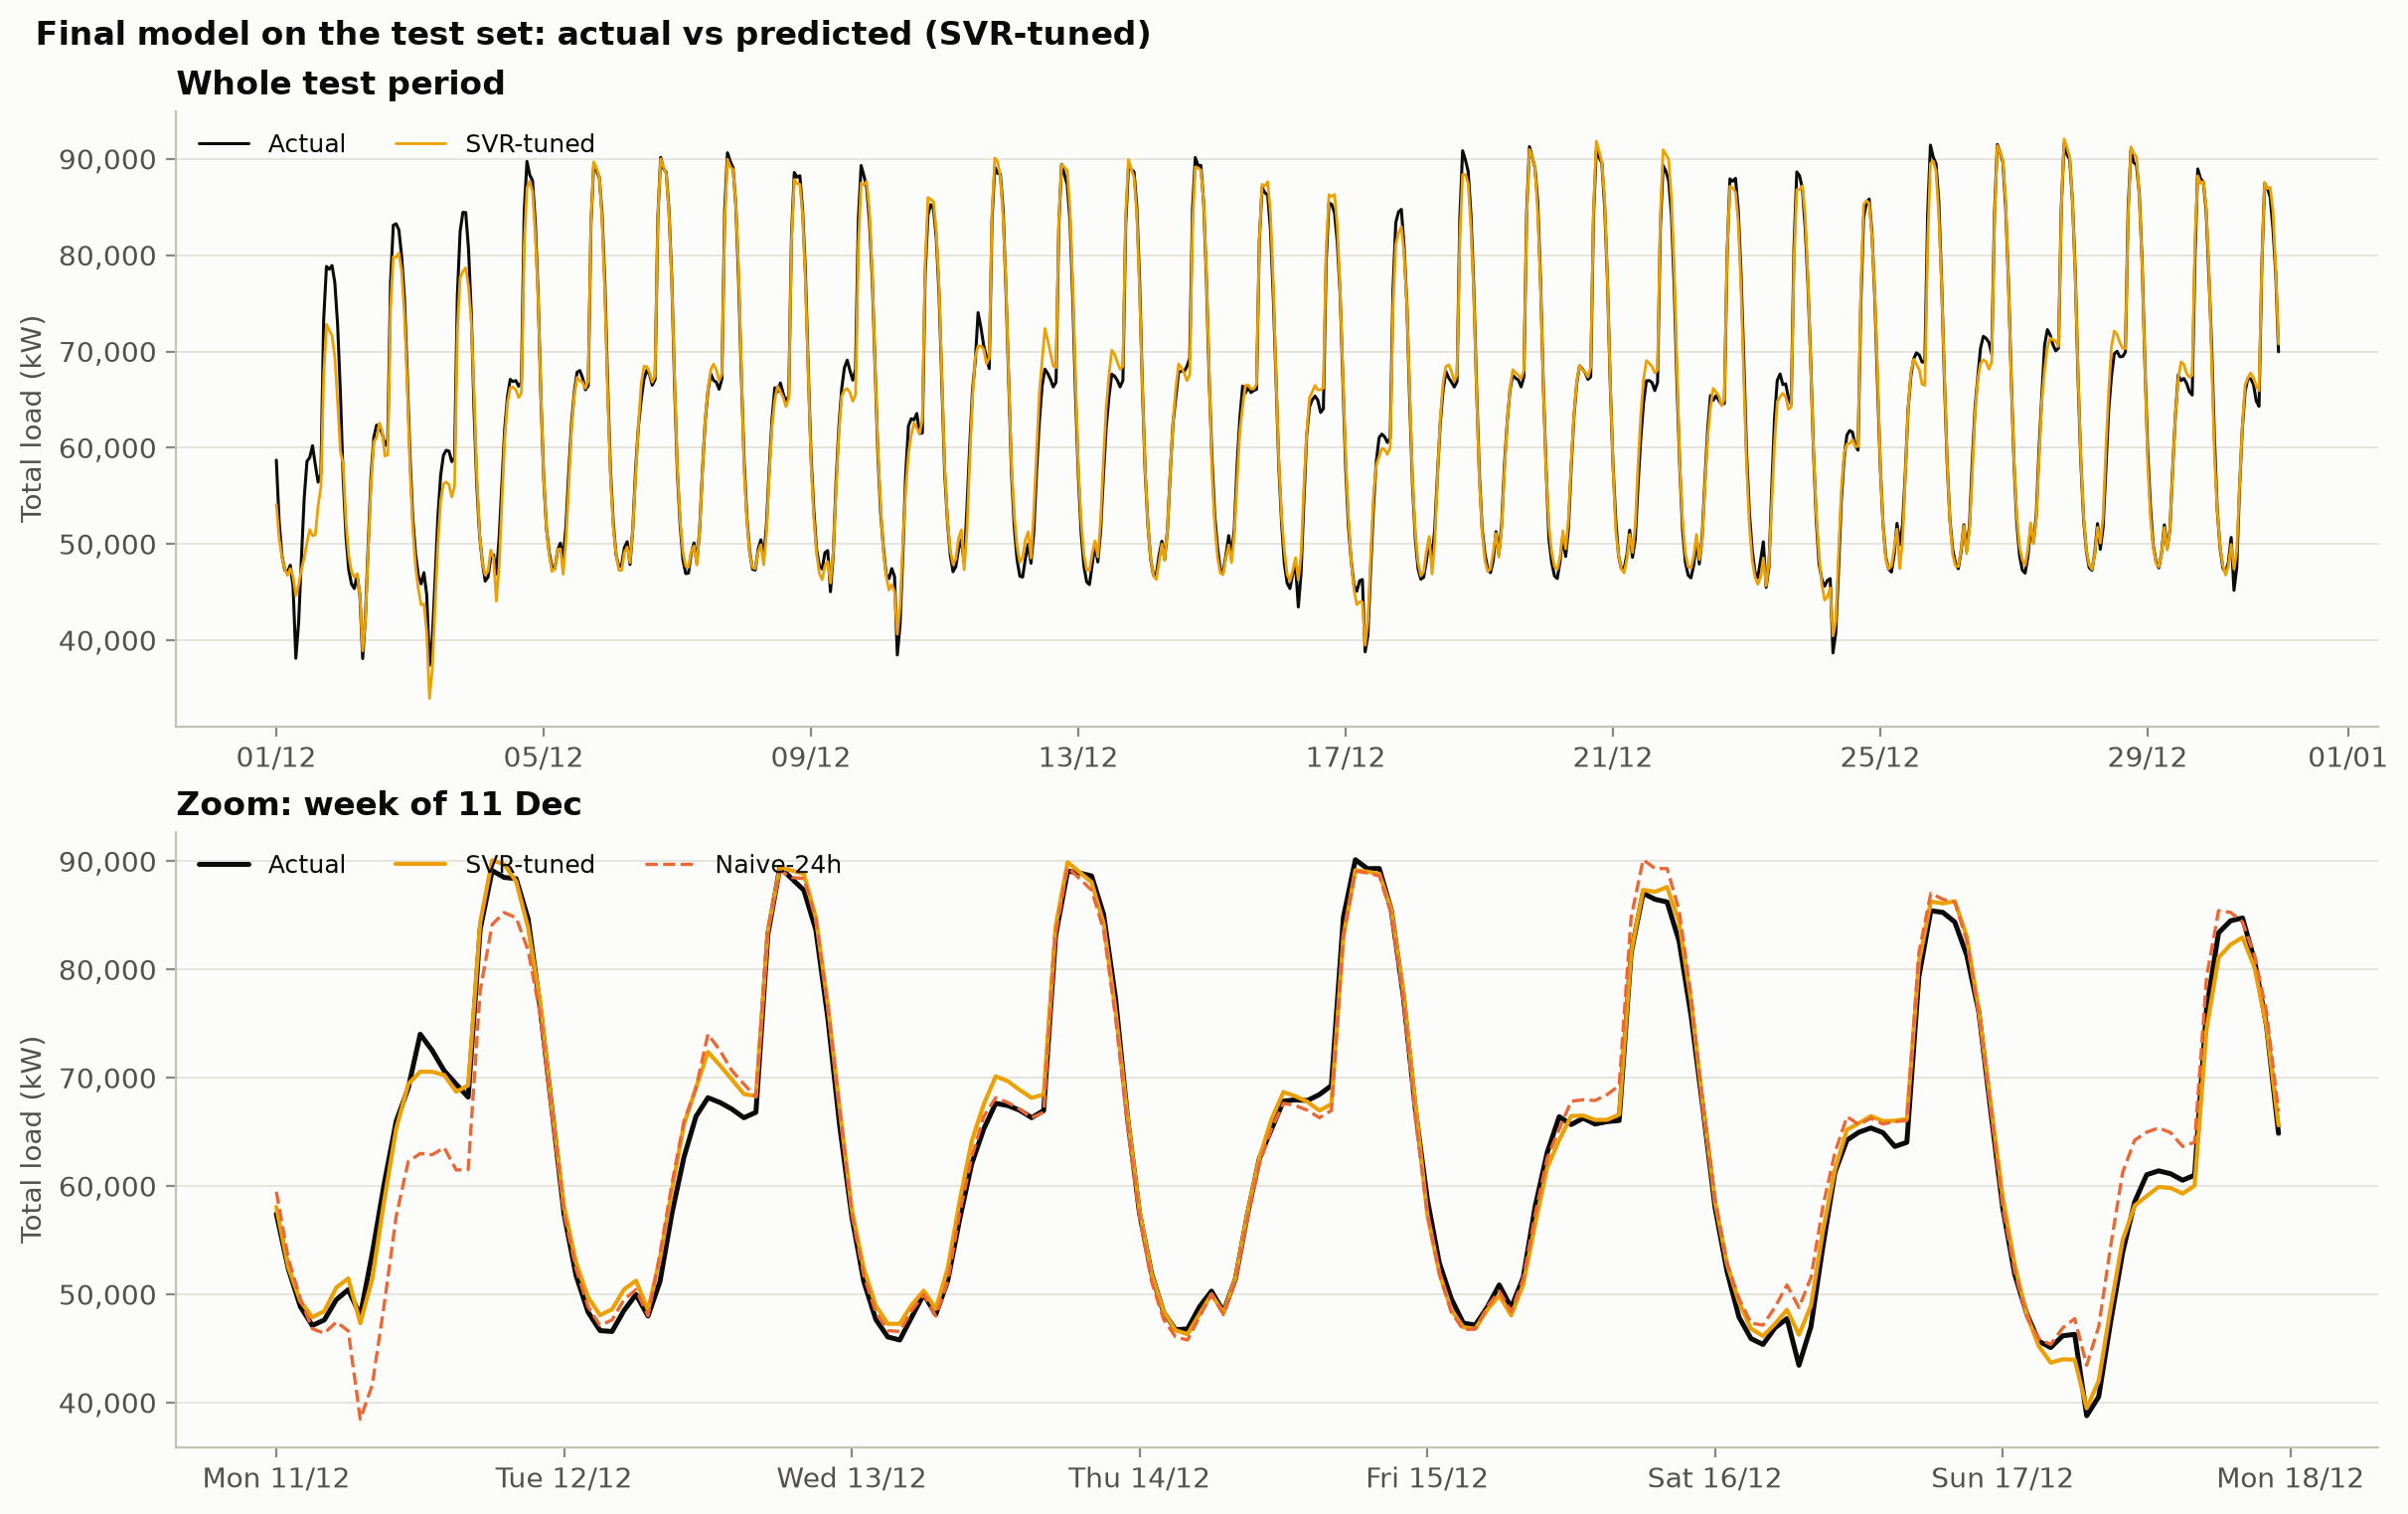
\includegraphics[width=\linewidth]{F17_test_actual_vs_pred.png}
\caption{Actual and selected h24 SVR test forecasts, with an 11--17 December zoom and the daily naive reference (F17). Measurements from completed prior days update the load-history inputs throughout the month.}\label{fig:test_series}
\end{figure}
\begin{figure}[tbp]\centering
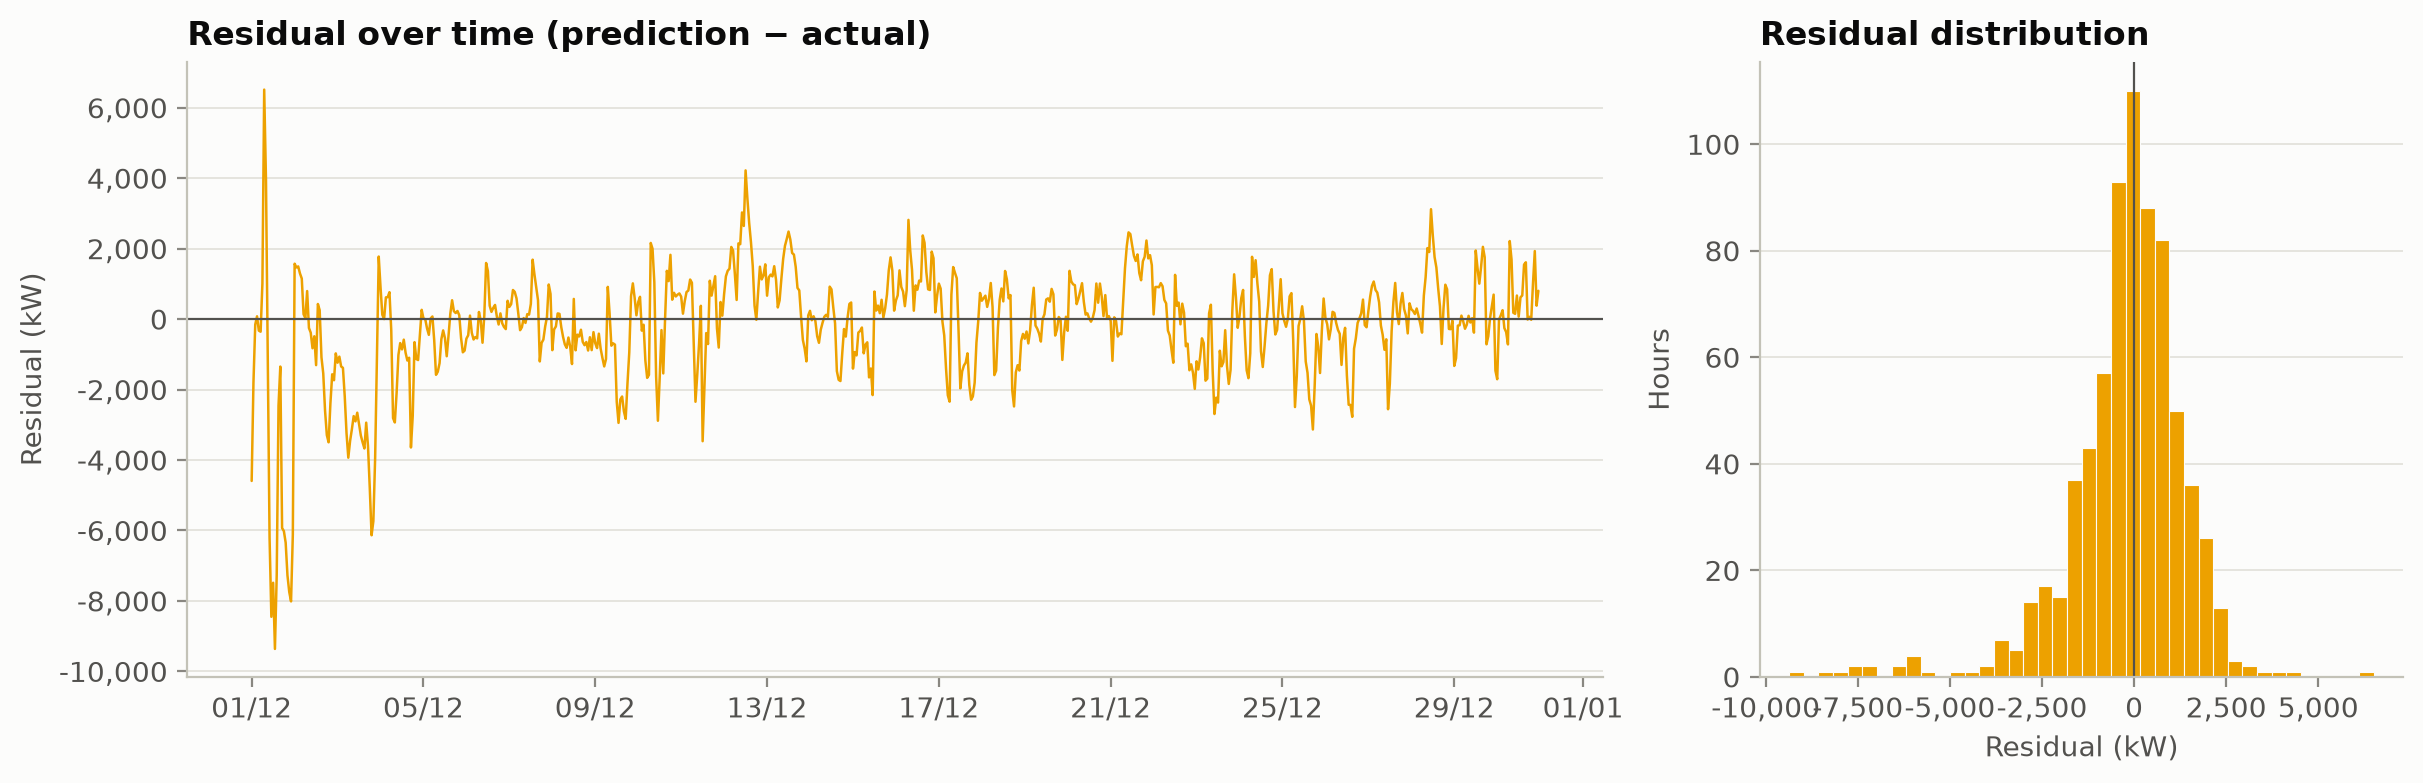
\includegraphics[width=\linewidth]{F17b_residuals.png}
\caption{Selected h24 SVR errors over December and their empirical distribution (F17b). Negative errors indicate underprediction. The early-month negative tail warrants attention despite the small average bias.}\label{fig:test_residuals}
\end{figure}

The mean December load is \num{63750.8} kW. MAE divided by this mean is about \num{1.72}\%, which differs from MAPE, \num{1.78}\%, because MAPE divides each error by its own observation before averaging. \Cref{fig:test_groups} reveals that improvements over Naive-24h vary across groups. Nonholiday Monday MAE is approximately \num{1007} versus \num{5294} kW, whereas Wednesday MAE is approximately \num{710} versus \num{562} kW: the selected model is not better in every subgroup.
\begin{figure}[tbp]\centering
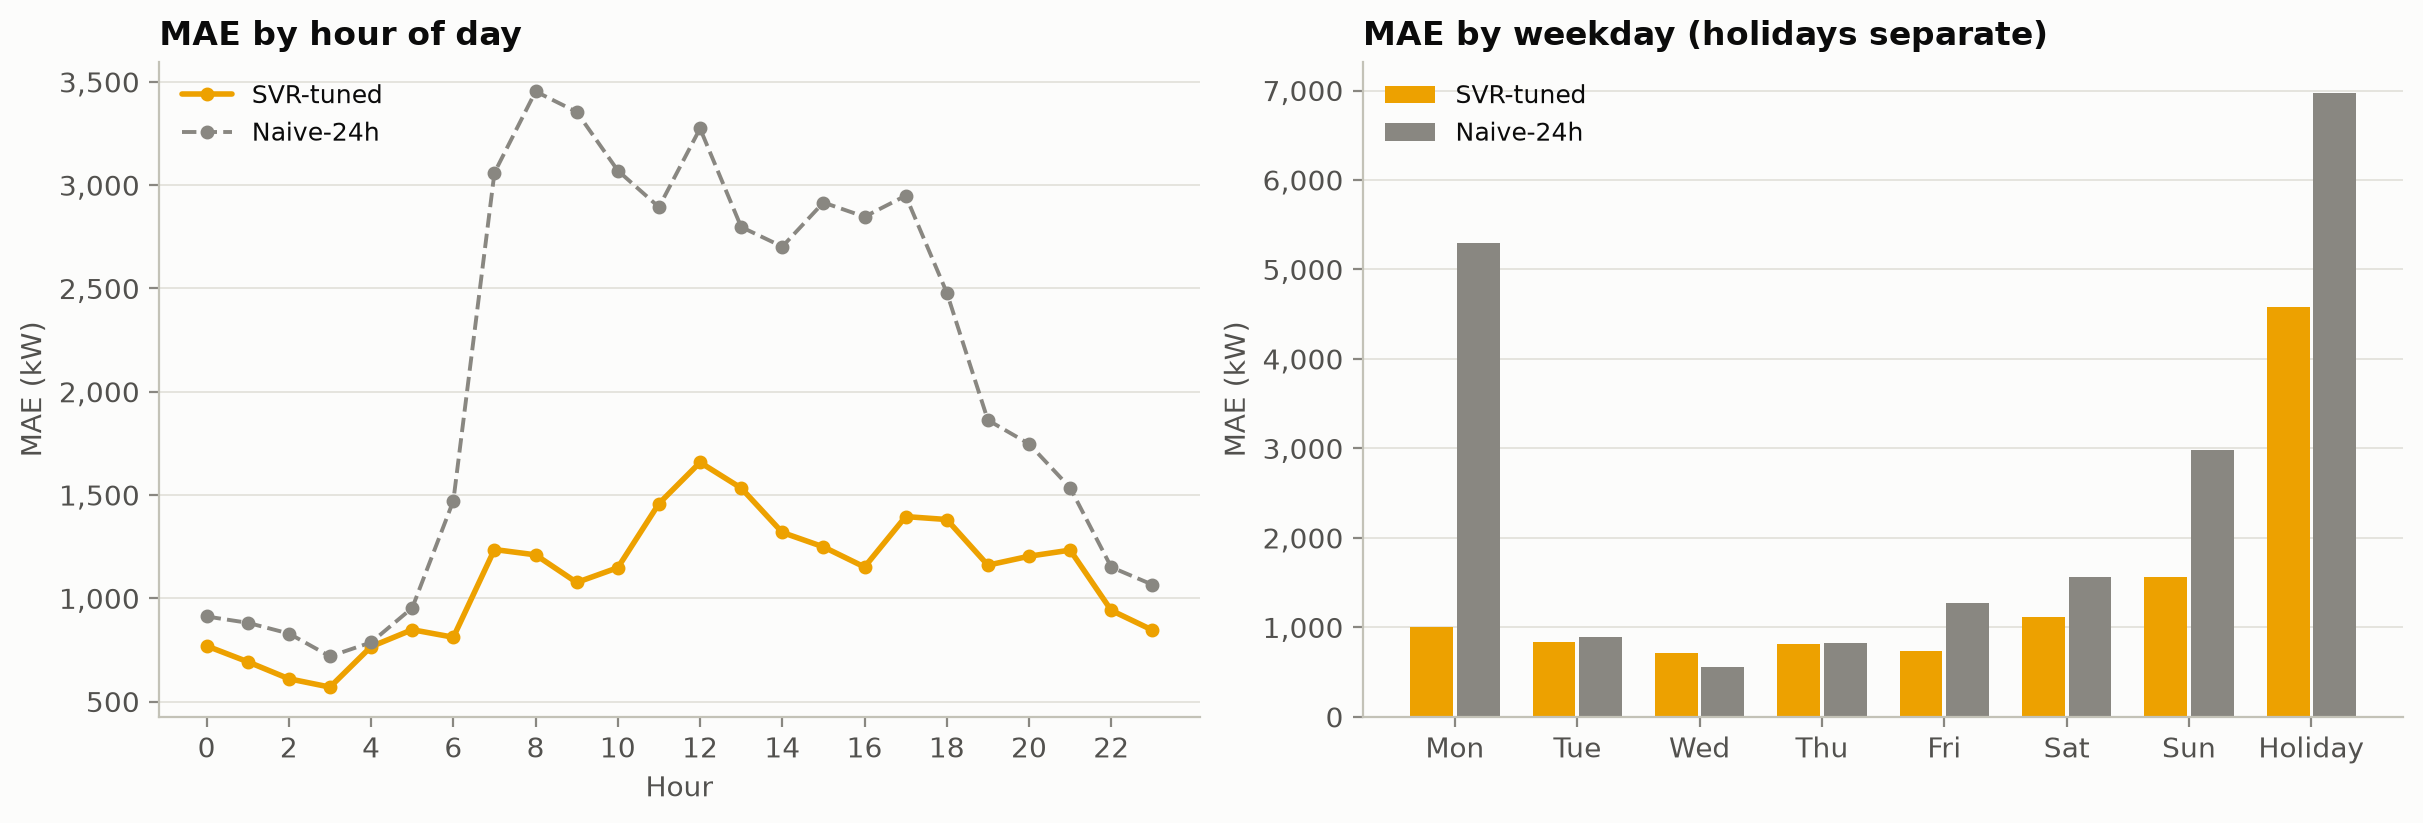
\includegraphics[width=\linewidth]{F18_error_by_hour_weekday.png}
\caption{December MAE by hour and weekday for selected h24 SVR and Naive-24h (F18). Holidays are separated from weekdays; the holiday group contains only 1 December, limiting generalization of that comparison.}\label{fig:test_groups}
\end{figure}

\Cref{tab:worst_days} identifies 1 December, marked as Mawlid in the implemented calendar, as the largest daily-error case: MAE \num{4579.2} kW and bias $-\num{3616.7}$ kW. The forecast daily mean is \num{54957.4} kW against actual \num{58574.2} kW. A shared religious-holiday indicator learned from different events may inadequately represent this date. This is a hypothesis suggested by the feature design and saved analysis, not an isolated intervention test. Sunday 3 December is the next-worst day. Neither these diagnoses nor an error recalculated after excluding difficult dates should replace the complete test result.
\begin{table}[tbp]\centering\small
\caption{Five largest daily MAEs for the selected h24 SVR (T08). Bias is prediction minus actual; all numerical columns are in kW.}\label{tab:worst_days}
\setlength{\tabcolsep}{4pt}
\begin{tabular}{lrrrr}
\toprule
Date & MAE & Bias & Actual mean & Predicted mean \\
\midrule
2017-12-01 & \num{4579.2} & \num{-3616.7} & \num{58574.2} & \num{54957.4} \\
2017-12-03 & \num{3028.5} & \num{-2880.5} & \num{59192.4} & \num{56311.9} \\
2017-12-12 & \num{1714.1} & \num{1712.5} & \num{64338.5} & \num{66051.1} \\
2017-12-21 & \num{1336.2} & \num{1118.1} & \num{64373.9} & \num{65492.0} \\
2017-12-02 & \num{1273.4} & \num{-554.7} & \num{60104.3} & \num{59549.7} \\
\bottomrule\end{tabular}
\end{table}


\subsection{Interpretability of the CV-preferred tree model}
The explanatory analysis uses residual RF, the tree candidate with the lowest development mean CV RMSE, rather than the selected SVR. \Cref{fig:importance,fig:shap} therefore describe a different estimator. Built-in importance measures impurity reduction within the residual forest; permutation importance measures the RMSE increase of the complete base-plus-correction predictor after shuffling a test column. Ten repeats with seed 42 are used in the full saved experiment.
\begin{figure}[tbp]\centering
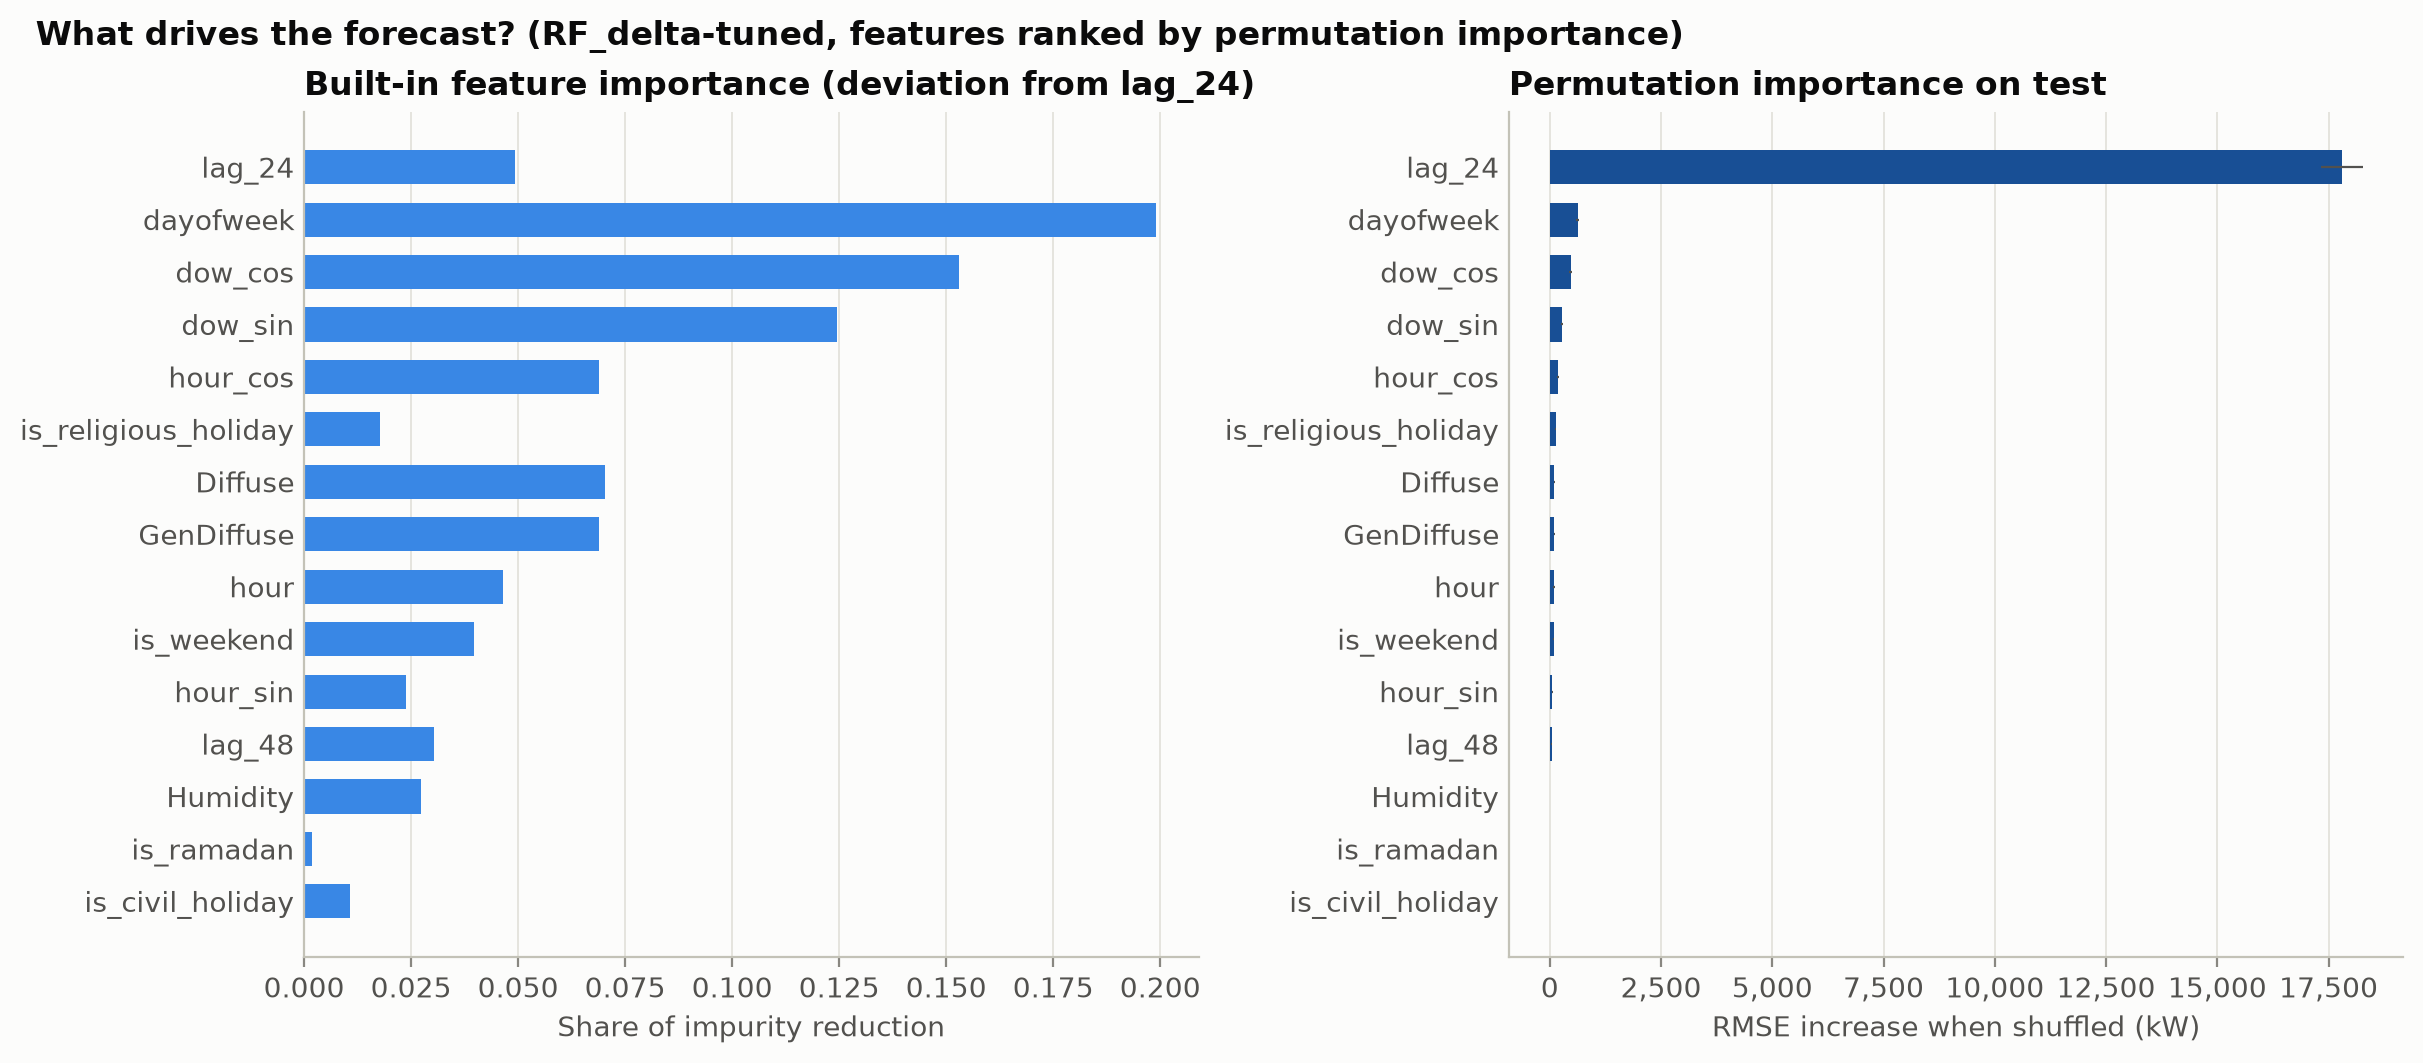
\includegraphics[width=\linewidth]{F19a_feature_importance.png}
\caption{Residual-RF built-in and test permutation importance (F19a). Built-in importance concerns the correction to lag-24; permutation importance concerns the full forecast. Shuffling lag-24 also changes the explicit forecast base, so the two panels measure different quantities.}\label{fig:importance}
\end{figure}
\begin{figure}[tbp]\centering
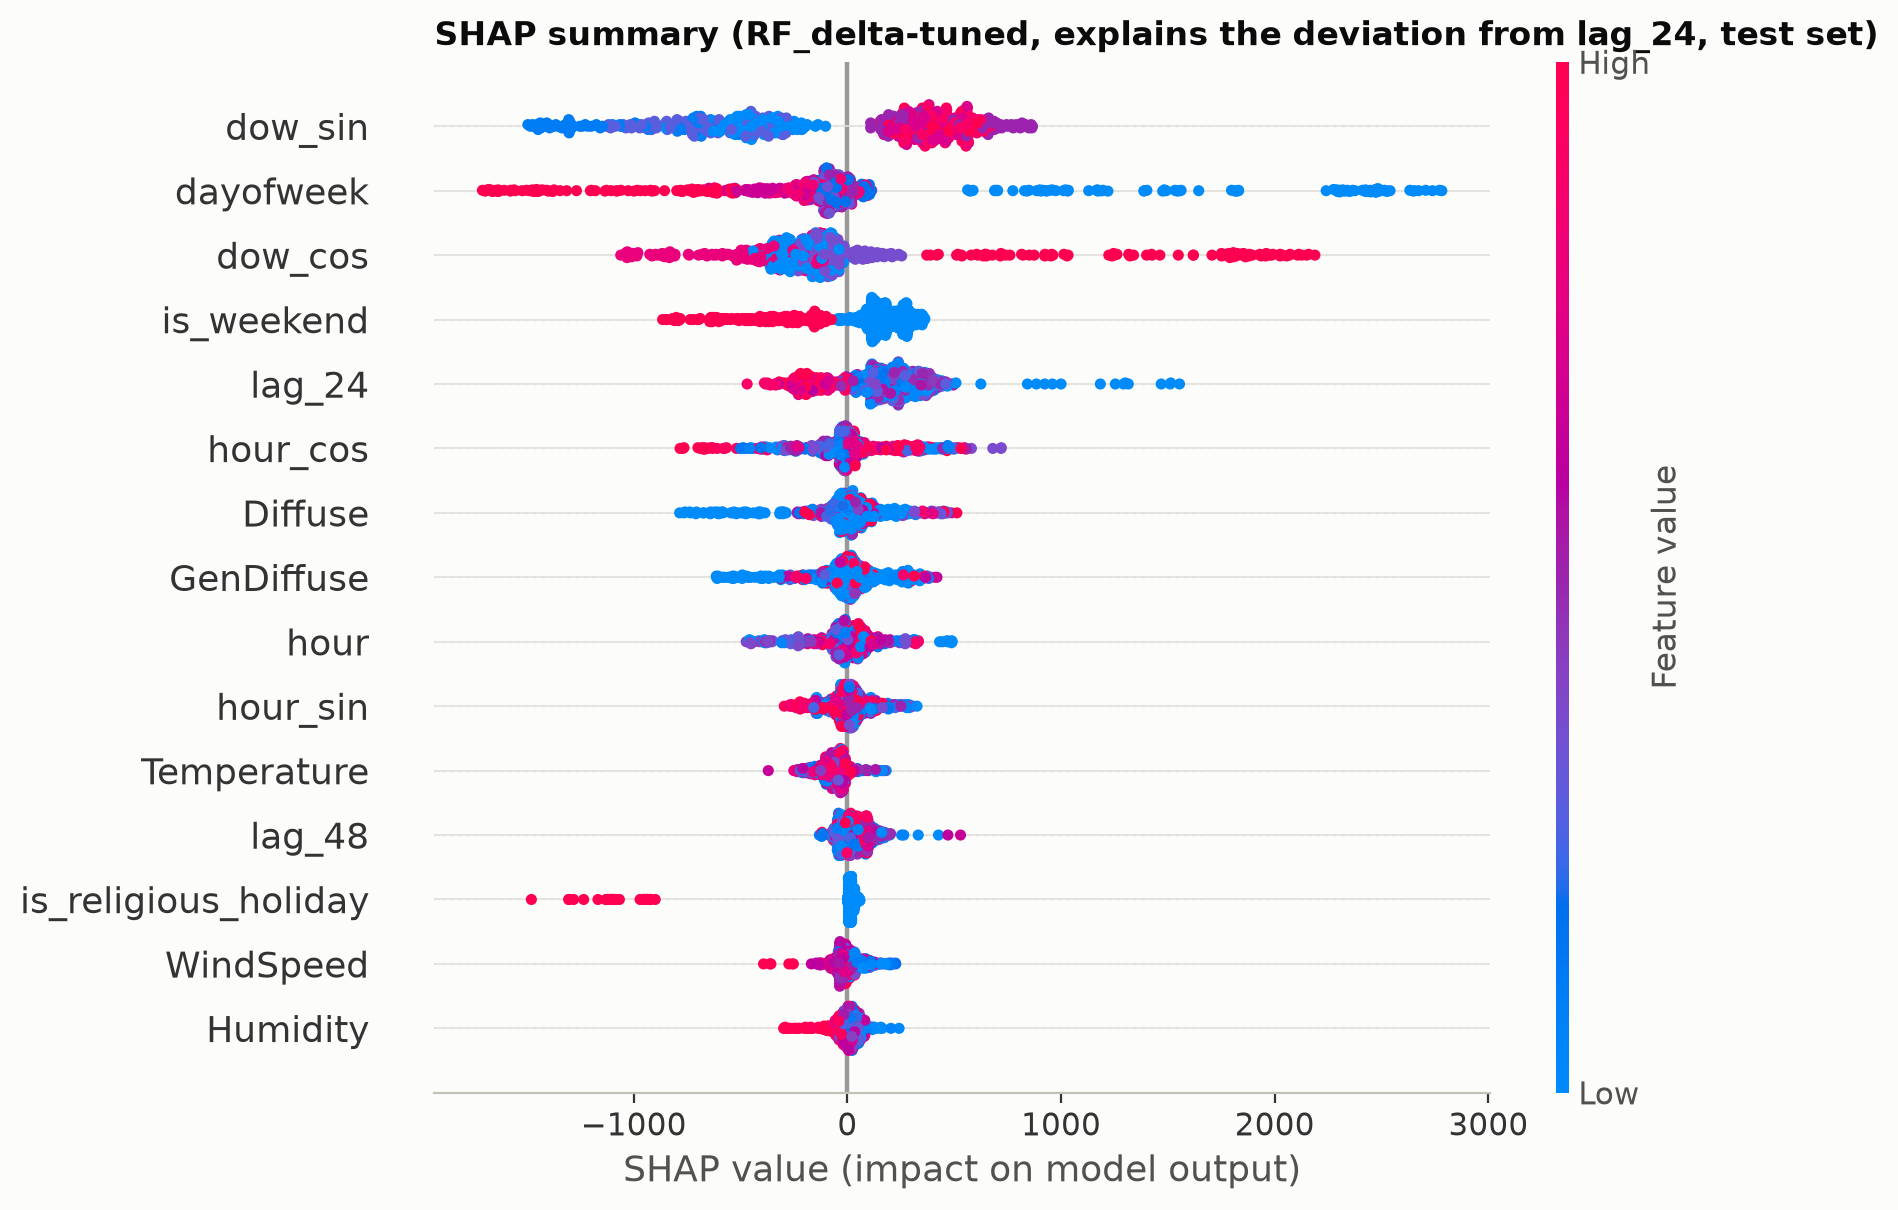
\includegraphics[width=.88\linewidth]{F19b_shap_summary.png}
\caption{Tree SHAP summary for the residual RF on December inputs (F19b). Contributions are in kW of the learned correction, not the complete load or the selected SVR output.}\label{fig:shap}
\end{figure}

SHAP decomposes model predictions into feature contributions\cite{lundberg2017}. Here the tree explainer sees only the residual ensemble, so it excludes the separate additive base $y_{t-24}$. Weekday encodings contribute prominently to the correction, while the large lag-24 permutation effect partly reflects its direct role in the complete prediction. Correlated lags and redundant calendar encodings can yield unrealistic combinations when independently permuted. These post-test diagnostics explain predictive behavior conditionally; they establish neither causal effects nor selected-SVR feature importance. No numerical SHAP-value table is archived. Additional scatter and dependence plots are retained in \cref{sec:supp_figures}.
\evidence{Notebook 07 cells 4--35; T08 final-test, prediction and worst-day files; T07/T10 selection scores; F17--F19; \code{docs/progress.md} and \code{docs/result.md}, Section 11, for test reruns.}

\section{Data Leakage Investigation}\label{sec:leakage}
\subsection{Availability, chronology and what is verified}
For an issuance time $\tau$, an operational forecast should depend only on information available by $\tau$. Writing that information as $\mathcal I_\tau$, a deployable prediction satisfies $\widehat y_t=f(\mathcal I_\tau)$ for a future target interval $t$. A feature can precede its target in a DataFrame while still be unavailable at the intended issuance time. Conversely, a future calendar value is normally known in advance and is not leakage merely because its date lies after training.

The pipeline implements several verified protections: chronological fit/evaluation partitions; training-fitted input and target scaling; training-only mean profiles; shifted load lags and rolling windows; and numerical checks of history construction. Notebook 02 deliberately inserts an unshifted rolling feature and detects it. This negative test establishes that the checker catches that construction error; it does not show that the final model uses the deliberately corrupted feature. No main-model same-hour zone input or unshifted target-derived rolling predictor was found.

Target-hour weather is a distinct, confirmed availability mismatch for advance forecasting. Its hourly average is observed during the interval being predicted and is passed to the model without shifting. It is not an archived weather forecast available at midnight or before the next hour. If the reported scores were presented as fully operational advance forecasts, this would constitute look-ahead information. Under the explicitly stated oracle-weather experiment, the scores instead describe conditional predictive performance; the deployment limitation remains real and unquantified. The weather-free tree ablation does not resolve it for the selected SVR.

Immediate delivery of completed-hour load measurements is another assumption, rather than a verified data-service capability. The notebook checks historical indices, not acquisition latency. Full-year descriptive EDA, development-fold reuse and documented test reruns additionally weaken claims of an independently hidden test. These limitations should be stated separately from an assertion that evaluation labels were directly used to fit the main estimator, which the inspected training code does not show.

\subsection{S1--S4 design}
Notebook 08 conducts diagnostics after final evaluation. The same absolute RF parameter values are used in S1--S4: 200 trees, maximum depth 30, minimum leaf size two and feature fraction 0.8. Input dimensions differ, so that fraction can correspond to different numbers of candidate split features. \Cref{tab:leakage} records sample counts and metrics.

S1 uses ten-minute observations with five weather variables and eight calendar fields: month, day, hour, minute, day of year, week of year, weekday and quarter. After the common initial lag-related row removal, \num{52415} rows are randomly split 75/25 with seed 42. S2 uses the same shuffled split and adds the immediately previous ten-minute load. S3 uses chronological fitting before December and evaluates all \num{4320} December ten-minute targets; it retains the short lag, removes day of year, and retains the other calendar fields, including month and day. S4 returns to the 17-feature hourly h24 pipeline with \num{7825} development and 720 test rows.
\begin{table}[tbp]\centering\small
\caption{Four RF diagnostic settings (T12). These rows differ in task and test distribution and must not be treated as a controlled leakage-effect estimate. Errors in kW.}\label{tab:leakage}
\setlength{\tabcolsep}{4pt}
\begin{tabular}{lrrrrrr}
\toprule
Setting & Train / test rows & Features & RMSE & MAE & MAPE (\%) & R$^2$ \\
\midrule
S1 & \num{39311} / \num{13104} & \num{13} & \num{1325.3} & \num{854.8} & \num{1.25} & \num{0.9940} \\
S2 & \num{39311} / \num{13104} & \num{14} & \num{620.0} & \num{419.2} & \num{0.61} & \num{0.9987} \\
S3 & \num{48095} / \num{4320} & \num{13} & \num{644.0} & \num{443.3} & \num{0.74} & \num{0.9980} \\
S4 & \num{7825} / \num{720} & \num{17} & \num{2017.1} & \num{1331.7} & \num{2.19} & \num{0.9798} \\
\bottomrule\end{tabular}
\end{table}


S1 achieves RMSE \num{1325.3} kW and MAPE \num{1.25}\%; S2 achieves \num{620.0} kW and \num{0.61}\%. S3 reaches \num{644.0} kW and \num{0.74}\%, while S4 reaches \num{2017.1} kW and \num{2.19}\%. S4 reproduces the absolute tuned RF result in \cref{tab:test24}; it is not the selected SVR's test score. \Cref{fig:leakage_settings} plots MAPE and unexplained variance, $1-R^2$, for these same rows.
\begin{figure}[tbp]\centering
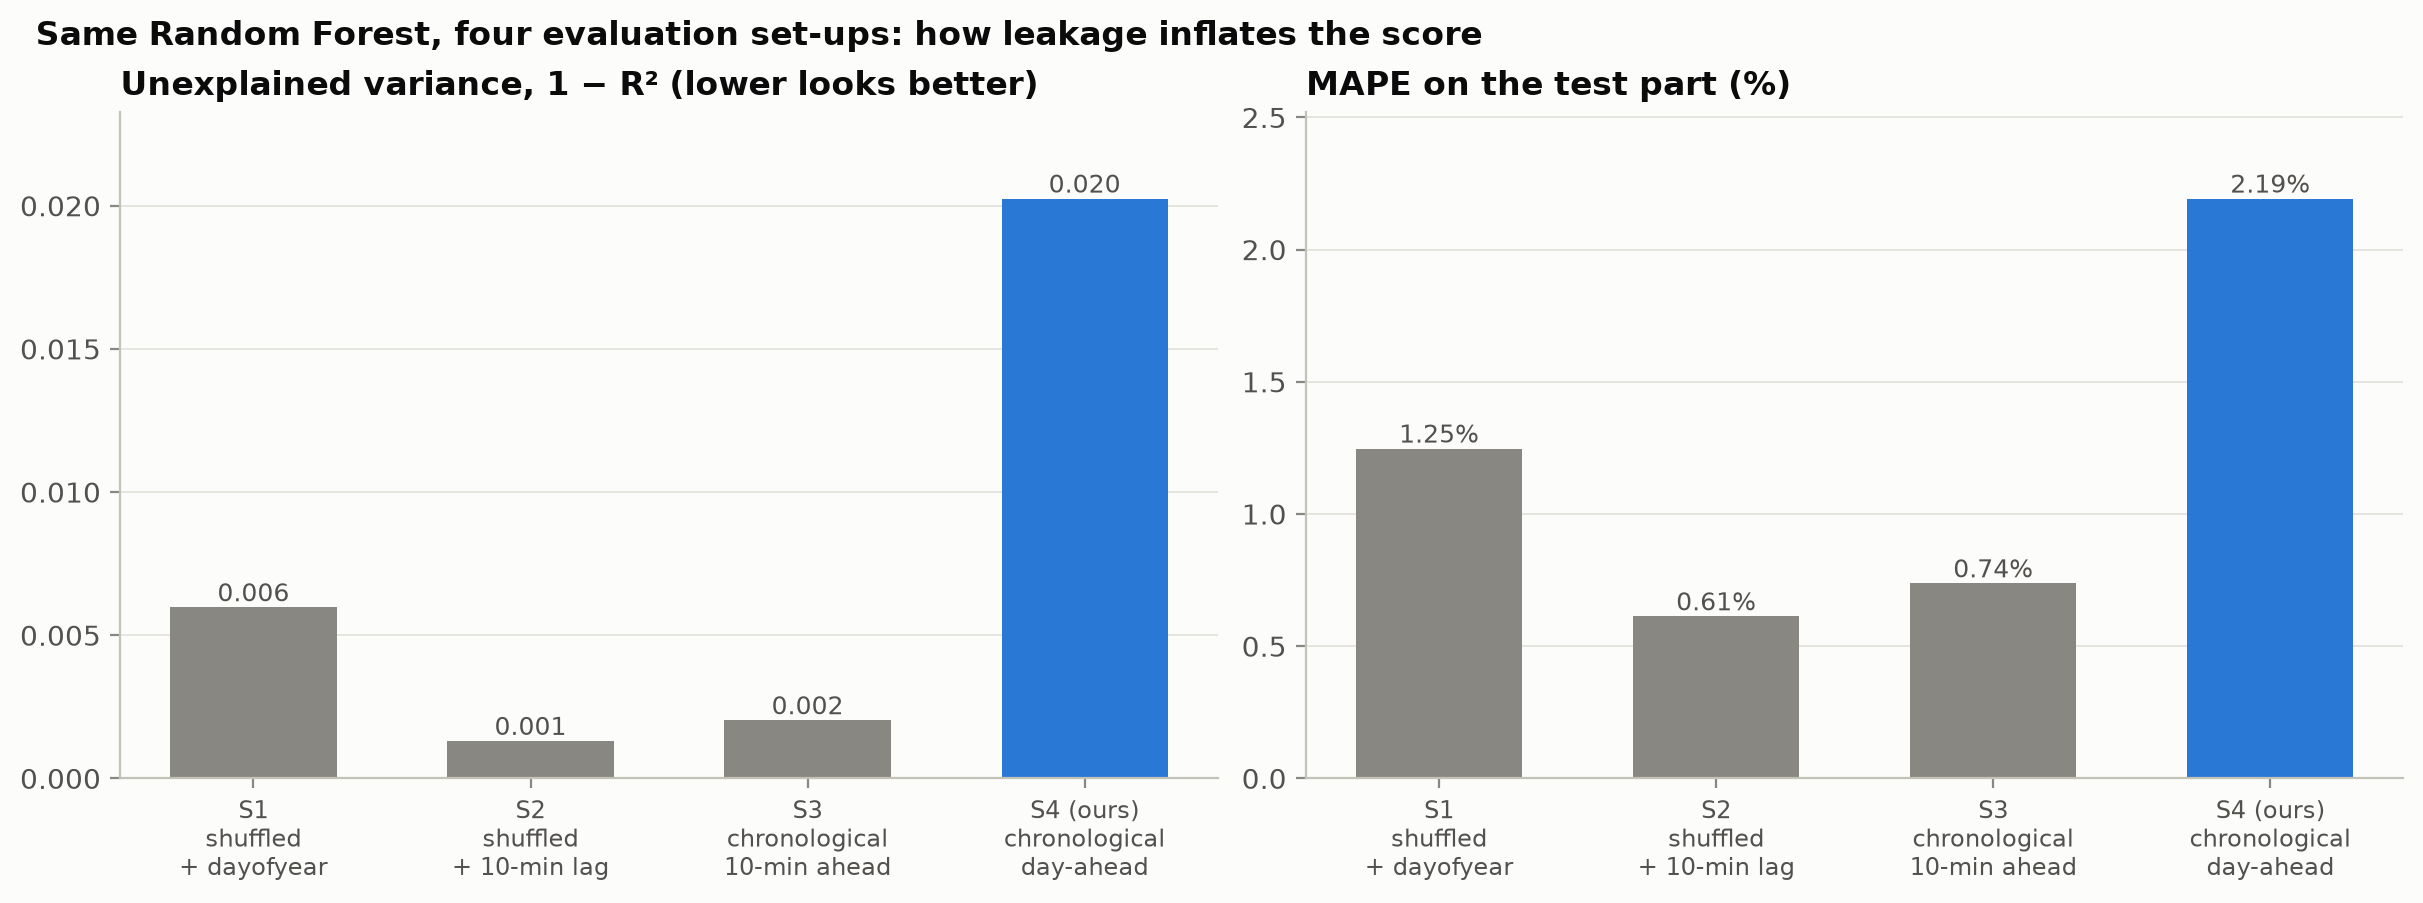
\includegraphics[width=\linewidth]{F16_leakage_settings.png}
\caption{RF diagnostic results under four evaluation settings (F16). The original image title attributes score inflation to leakage; the experiment changes split, features, target resolution and forecast horizon, so the bars do not isolate a leakage effect.}\label{fig:leakage_settings}
\end{figure}

\subsection{What the diagnostic comparisons establish}
Shuffled training can contain dates later than an evaluated target, including temporally nearby observations. This violates a past-only fitting protocol for prospective forecasting and favors interpolation within an observed year. S2 additionally has a concrete route by which held-out responses enter fitting inputs: its lag is constructed before splitting, so a held-out $y_t$ becomes \code{lag_10min} in the training row at $t+10$ minutes whenever that successor is assigned to training. Reconstructing only the saved seed-42 row split verifies \num{9834} such held-out responses among \num{13104} test rows. This is a dependency across the shuffled holdout boundary, not evidence that the main chronological model was fitted on December responses. Legitimately updating past observations during chronological forecasting has a different information ordering.

S1--S4 do not estimate how much of their score difference is caused by either leakage mechanism. S1 versus S2 changes one feature within the shared shuffled setting, but that added lag introduces both useful recent history and the cross-boundary response dependency; its accuracy benefit cannot be assigned to history alone. S2 versus S3 changes split, calendar inputs, training size and test population. S3 versus S4 changes resolution, historical inputs and the effective forecasting task. All settings also use contemporaneous observed weather.

A ten-minute-ahead forecast with an available lag is a legitimate shorter-horizon task. Month and day of year are known at prediction time, although a model trained on shuffled dates may learn within-year patterns that do not transfer to future periods. S1's absence of load lags does not alone rule out forecasting if suitable future covariates are available. The critical issues are predictor availability and whether the fitted/evaluated distributions match intended use.

RMSE and MAE retain the same kW unit across settings, but their targets represent different averaging intervals and test observations. MAPE and R$^2$ remove a common multiplicative scale; they do not equalize temporal resolution, target variation, forecast horizon or test difficulty. Consequently, neither the low ten-minute errors nor their ratios to S4 support a causal ``price of leakage'' or a universal correction factor for published scores.

\subsection{Shuffled KFold versus temporal model selection}
The supplementary RF experiment is more closely controlled: the h24 development data, feature set, seed, sampled search space and 20-candidate budget are common. It compares shuffled five-fold KFold with the existing expanding temporal folds, refits each selected configuration on development data, and evaluates December. This is a separate diagnostic search, not the main 30-candidate RF tuning result.
\begin{table}[tbp]\centering\small
\caption{Post-final RF search diagnostic: 20 candidates per CV strategy (T12b). Optimism is $100(\mathrm{RMSE}_{test}/\mathrm{RMSE}_{CV}-1)$. Errors in kW.}\label{tab:kfold}
\setlength{\tabcolsep}{4pt}
\begin{tabular}{lrrr}
\toprule
CV strategy & CV RMSE & December RMSE & Optimism (\%) \\
\midrule
KFold (shuffled) & \num{2007.6} & \num{2173.6} & \num{8.27} \\
TimeSeriesSplit & \num{3012.4} & \num{2044.2} & \num{-32.14} \\
\bottomrule\end{tabular}
\end{table}


As \cref{tab:kfold} shows, KFold selects a configuration with CV RMSE \num{2007.6} kW and December RMSE \num{2173.6} kW. The temporal search gives \num{3012.4} and \num{2044.2} kW. The table's signed discrepancy is
\begin{equation}
O=100\left(\frac{\mathrm{RMSE}_{\mathrm{December}}}{\overline{\mathrm{RMSE}}_{\mathrm{CV}}}-1\right),
\label{eq:optimism}
\end{equation}
giving $+\num{8.27}\%$ for KFold and $-\num{32.14}\%$ for temporal CV. In this realization, KFold is optimistic relative to December and selects a model with worse December RMSE. Temporal CV includes difficult summer windows and is more pessimistic for this test month. The fold strategies also differ in training sizes and validation populations; this is not repeated evidence of a universal bias magnitude.

The selected KFold RF has 300 trees, depth 20, minimum leaf size one and square-root feature sampling. The temporal counterpart has 500 trees, depth ten, minimum leaf size two and feature fraction 0.8. Their different test results illustrate that validation can change the selected estimator, not just the reported score. Because these diagnostics reuse December after final analysis, they are explanatory follow-up experiments and do not provide an additional independent holdout.

\subsection{Implications for trustworthy reporting}
The GitHub survey in \cref{tab:survey} documents heterogeneous practices and seven shuffled evaluations among ten entries. It is a repository-authored survey, not an independent reproduction of each project, and it cannot establish the prevalence of leakage across the wider literature. The present evidence supports documenting issuance, target resolution, covariate availability, temporal fitting and selection history alongside every accuracy result. A controlled future study would vary one factor at a time on matched targets and evaluate forecasts with an issuance-time weather archive. Such a study is not implemented here.
\evidence{Notebook 08 cells 4--17; T11, T12 and T12b; notebook 02 history checks; \code{src/features.py}; \code{docs/kaggle_survey.csv}; \code{report/evidence/peer_review_checks.json} for the index-only S2 dependency check. No model was refitted for this verification.}

\section{Discussion}\label{sec:discussion}
\subsection{Answers to the research questions}
The first objective was to assess whether ML improves on seasonal rules under chronological evaluation. Several default models improve on Naive-24h in November, yet their ordering changes across temporal folds. LR is the strongest default by mean CV RMSE, while tuning selects absolute SVR. The selected h24 SVR reduces December RMSE by \num{50.71}\% against the daily naive reference and also improves on the weekly reference. Thus improvement is supported within the observed evaluation setting, rather than as an unconditional ranking of algorithms.

The feature experiments show that daily history is the most effective sequential addition tested for RF/XGB. Calendar variables help represent recurring demand differences, but weather and calendar inputs without load history remain poor substitutes for a recent measured level. Weekly and rolling summaries worsen results under D-selected parameters. The conclusion is to match feature construction to validation evidence; the study does not establish that weekly information is intrinsically useless or that the same subsets would win after independent retuning.

The residual formulation improves tuned development mean RMSE for four of five families, helping trees predict corrections around an available recent load. Absolute SVR remains slightly better in development for both settings. The different h24 test ordering shows why the choice must be retained separately from the observed test winner. The h1 configuration improves mean CV RMSE for each family representative, but its feature set, residual base and tuning differ from h24. The study supports this configuration-level finding without claiming a controlled lead-time response curve.

\subsection{Accuracy, complexity and practical cost}
\Cref{tab:runtime} gives the recorded h24 refit and prediction durations. The selected SVR takes approximately \num{3.686} s to fit and \num{0.137} s to predict 720 rows. Residual RF and residual XGB have shorter recorded fits, approximately \num{0.107} and \num{0.146} s, with test RMSEs \num{1761.9} and \num{1719.2} kW. Their development RMSEs are also close to SVR's. These alternatives may be relevant if latency or tree-based explanations matter, but the experiment does not apply a formal multi-objective selection rule.
\begin{table}[tbp]\centering\small
\caption{Recorded h24 refit and whole-test prediction durations for selected representative models (T08). Hardware and thread configuration are not recorded in this table; timings are descriptive.}\label{tab:runtime}
\setlength{\tabcolsep}{4pt}
\begin{tabular}{lrrr}
\toprule
Model & Fit (s) & Predict 720 rows (s) & Test RMSE (kW) \\
\midrule
LR $\Delta$-tuned & \num{0.003} & \num{0.001} & \num{2217.3} \\
DT $\Delta$-tuned & \num{0.015} & \num{0.001} & \num{2005.2} \\
RF $\Delta$-tuned & \num{0.107} & \num{0.026} & \num{1761.9} \\
SVR-tuned & \num{3.686} & \num{0.137} & \num{1624.6} \\
XGB $\Delta$-tuned & \num{0.146} & \num{0.003} & \num{1719.2} \\
\bottomrule\end{tabular}
\end{table}


The timings are single recorded runs without hardware provenance, repeated benchmarking or a consistent deployment service. They do not establish production throughput or scaling to larger datasets. Likewise, the reported number of search fits describes computational work, not an energy or monetary cost measurement. The uncomplicated seasonal and linear references remain useful as cheap diagnostics and potential fallback models, although a fallback policy was not implemented.

\subsection{Validation reliability and generalization}
Expanding folds expose summer errors hidden by a November-only evaluation. This is a concrete benefit of temporal validation, not a guarantee of future generalization. Fold scores combine seasonal difficulty with increasing training sizes, and reuse for feature choices and tuning creates selection bias. The narrow spread among leading tuned means is much smaller than their temporal dispersion; neither a significant winner nor statistical equivalence has been demonstrated.

The final evaluation covers a single 30-day period in one city/year. Its lower error than average development CV cannot represent all seasons. The early-December holiday failure also indicates that broad special-day categories may pool events with different demand responses. Sparse holiday occurrences prevent a reliable event-specific performance estimate. No zone-level forecasting results, multi-year transfer study, forecast intervals or external-city validation are available.

The measurement context further limits deployment claims. Observed target-hour weather overstates available information for advance forecasting unless replaced by an issuance-time forecast. Historical-load delivery latency and clock conventions are unspecified. Test reruns and descriptive exposure to December prevent certifying a fully hidden one-shot evaluation, even though the selection expression uses development scores. These are material boundaries on what the current evidence demonstrates.

\subsection{Relationship to verified prior work}
The literature in \cref{tab:literature} provides methodological context. Salam and El Hibaoui motivate conventional regression comparisons\cite{salam2018}; da Silva and Meneses provide a chronological deep-learning comparison as described in the local review\cite{silva2023}; shift-based and lag-enriched approaches emphasize historical demand\cite{islam2025,alsalem2025}; and the Darts study illustrates comparison across model families and resolutions\cite{biswas2026}. The present findings are consistent with the usefulness of history and careful validation, but those studies do not share a verified common target, lead, covariate-availability protocol and test period with this implementation.

For example, a zone-level ten-minute MAE cannot be ranked directly against an hourly three-zone total MAE. Taking the mean of three zones rather than their sum changes numerical scale, but correcting that scale alone does not align horizons or evaluation distributions. The report therefore retains traceable study descriptions and unavailable entries instead of constructing a cross-study leaderboard. F20 is not reproduced because its heterogeneous bar comparisons could encourage precisely that interpretation. No state-of-the-art conclusion follows.

\subsection{Implications and remaining evidence gaps}
For a practical forecasting workflow, the strongest supported lessons are to retain seasonal baselines, define the issuance schedule, audit every predictor's availability, and keep model-selection scores separate from final test observations. Interpretability should identify which estimator and output it explains: the saved Tree SHAP plots describe residual RF, not the selected SVR. Permutation experiments on correlated calendar/history columns should be treated as model diagnostics rather than causal importance.

Further claims require evidence absent from this snapshot: weather forecasts as issued, measured data latency, independently reserved seasonal/yearly tests, per-zone experiments, repeated computational benchmarks, uncertainty estimates and archived h1 forecast series. Some historical side experiments are described in documentation without their full fold/search artifacts. They can explain development rationale but cannot substitute for reproducible numerical evidence. All these gaps are recorded in the research audit rather than filled by new experiments for this report.
\evidence{T04--T10; T12/T12b; related-work evidence in \code{research_audit.md}; \code{docs/result.md}, Section 11; recorded runtimes in T08.}

\section{Conclusion and Future Work}\label{sec:conclusion}
This project evaluates conventional machine learning for hourly total electricity load in Tetouan using \num{52416} ten-minute observations aggregated into \num{8736} hourly means. Its contribution is a documented experimental pipeline combining seasonal references, chronological partitions, five expanding development folds, randomized parameter search, residual-target comparisons, feature ablation and evaluation diagnostics.

Absolute-target SVR minimizes development mean CV RMSE in both implemented settings. On the separate December period, the selected h24 model achieves RMSE \num{1624.6} kW and MAPE \num{1.78}\%, reducing RMSE by \num{50.71}\% against Naive-24h. The selected h1 model reaches RMSE \num{1195.8} kW and MAPE \num{1.41}\%. Residual SVR has lower observed h24 test RMSE, \num{1419.1} kW, but remains a test-best observation rather than a replacement for the CV-selected model.

The experiments show why feature and evaluation choices matter alongside algorithm choice. Daily lags provide the largest tested sequential feature improvement for RF/XGB; adding weekly and rolling summaries can worsen their scores under fixed D-selected parameters. Residual targets help most tuned families on development, while temporal folds reveal summer weaknesses missed by a single November split. S1--S4 demonstrate sensitivity to task and protocol, but their simultaneous changes prevent attributing the entire score difference to leakage.

These findings are conditional on observed target-hour weather and rapidly available historical loads. One year, one December holdout, reused development folds, descriptive test exposure and documented test reruns limit generalization claims. The report consequently supports accurate reporting under explicit information assumptions, rather than superiority over heterogeneous published results or deployment readiness.

Future work should first replace oracle weather with forecasts archived at issuance and incorporate measured load-delivery delays. A further independent year or several rolling seasonal holdouts would allow evaluation of summer peaks and holiday behavior after freezing development choices. Nested temporal selection or an additional outer validation layer could separate tuning from performance estimation. Retuned weather-free and weekly-feature ablations, with matched samples and availability, would better assess feature utility.

Additional horizons and explicitly stated issuance-to-target leads would clarify the relation between forecast difficulty and available history. Candidate extensions include classical time-series and alternative ML models, event-specific calendar encodings, per-zone forecasting, uncertainty intervals and explanations for the selected SVR. A later deployment study should assess monitoring, drift, fallback rules and computational cost. These are proposed investigations; none is presented as an implemented result of the current repository.

\FloatBarrier
\printbibliography[heading=bibintoc,title={References}]
\clearpage
\appendix
\section{Supplementary Reproducibility Material}\label{sec:supplementary}
\subsection{Artifact-based reproduction}
The report is reproducible from the saved numerical tables and existing figures without fitting models. From the repository root, \code{python report/build_tables.py} regenerates the report's table fragments and source map. \code{python report/check_evidence.py} independently checks stored numerical evidence, including all h24 prediction columns, without executing notebooks. The complete-report validator checks inputs, labels, citations and source hashes. Compilation commands and the precise scope of each helper are documented in \code{report/README.md}.

The evidence extracts retain PDF page boundaries and notebook cell indices. \code{source_manifest.json} records hashes of the audited project artifacts, \code{table_sources.json} maps generated tables to CSV/JSON inputs, and \code{research_audit.md} maps important narrative claims. The report-generation helpers write within \code{report/}; they do not regenerate project experiments. The notebook runner is intentionally excluded from this compilation workflow because normal execution would fit models and overwrite saved notebook/results outputs.

\subsection{Recorded environment and experiment execution}
\Cref{tab:dependencies} reproduces the dependency pins recorded by the repository. Its experiment environment is documented as Python 3.12 with seed 42. The report inspection environment is distinct and was not used to refit the results. Package pins are provenance statements; this report does not certify that a fresh environment was installed or every artifact was reproduced end to end.
\begin{table}[H]\centering\small
\caption{Recorded experiment dependencies from requirements.txt; Python 3.12 is specified by the repository. These are recorded pins, not a newly reproduced environment.}\label{tab:dependencies}
\setlength{\tabcolsep}{4pt}
\begin{tabular}{ll}
\toprule
Package & Pinned version \\
\midrule
numpy & 2.5.3 \\
pandas & 3.0.6 \\
scipy & 1.18.1 \\
scikit-learn & 1.9.1 \\
xgboost & 3.4.1 \\
statsmodels & 0.15.0 \\
shap & 0.52.0 \\
matplotlib & 3.11.2 \\
seaborn & 0.13.2 \\
jupyter & 1.1.1 \\
ipykernel & 7.4.0 \\
nbformat & 5.11.1 \\
nbclient & 0.11.0 \\
\bottomrule\end{tabular}
\end{table}


The documented notebook order is EDA, features, November baselines, temporal CV, tuning, ablation/horizon, final test analysis and leakage diagnostics. \code{TETOUAN_N_JOBS} controls search parallelism. Smoke mode changes periods and model/search budgets and writes separate outputs under \code{results/smoke/}; its scores are code-check outputs, not the reported experiments. No full or smoke experiments were executed to prepare this report. Hardware, exact execution history, model binaries and h1 individual predictions are not archived.

\subsection{Repository organization}
\begin{verbatim}
Machine-Learning/
  README.md                 project overview
  requirements.txt          recorded experiment dependencies
  run_all.py                notebook execution runner
  data/                     existing data artifacts
  docs/                     guideline, literature review and logs
  notebooks/                ordered notebooks 01--08
  src/                      config, data, features, evaluate,
                            models, viz, and package initializer
  results/
    tables/                 saved CSV metrics/searches and JSONs
    figures/                existing PNG assets
  report/
    main.tex                root-relative LaTeX entry point
    references.bib          traceable bibliography
    research_audit.md       evidence and discrepancy audit
    sections/               thirteen report sections
    appendices/             supplementary material
    tables/                 generated LaTeX table fragments
    evidence/               extracts, manifests and checks
\end{verbatim}

\subsection{Supplementary metric variability}
\Cref{tab:cv_variability} gives mean and sample SD for every default-CV metric. These statistics describe temporal fold variation, not independent-seed repetitions. They complement the fold-specific RMSEs in \cref{tab:cv_folds}.
\begin{table}[tbp]\centering\small
\caption{Supplementary default CV variability for all four metrics (T05); mean $\pm$ sample SD. RMSE/MAE in kW, MAPE in percent.}\label{tab:cv_variability}
\setlength{\tabcolsep}{4pt}
\begin{tabular}{lrrrr}
\toprule
Model & RMSE & MAE & MAPE & R$^2$ \\
\midrule
LR & \num{2792.3} $\pm$ \num{623.3} & \num{2101.0} $\pm$ \num{468.9} & \num{2.949} $\pm$ \num{0.538} & \num{0.965} $\pm$ \num{0.016} \\
RF & \num{3069.5} $\pm$ \num{1488.8} & \num{2168.6} $\pm$ \num{985.0} & \num{2.824} $\pm$ \num{0.820} & \num{0.958} $\pm$ \num{0.030} \\
XGB & \num{3264.8} $\pm$ \num{1815.8} & \num{2328.0} $\pm$ \num{1161.3} & \num{2.992} $\pm$ \num{0.967} & \num{0.951} $\pm$ \num{0.043} \\
Naive-24h & \num{3392.4} $\pm$ \num{421.5} & \num{2371.7} $\pm$ \num{351.6} & \num{3.285} $\pm$ \num{0.318} & \num{0.950} $\pm$ \num{0.009} \\
SVR & \num{3968.7} $\pm$ \num{2891.5} & \num{2753.4} $\pm$ \num{1890.7} & \num{3.445} $\pm$ \num{1.591} & \num{0.922} $\pm$ \num{0.093} \\
DT & \num{4048.2} $\pm$ \num{1410.4} & \num{2915.3} $\pm$ \num{996.7} & \num{3.873} $\pm$ \num{0.768} & \num{0.929} $\pm$ \num{0.032} \\
Naive-168h & \num{4892.6} $\pm$ \num{2297.1} & \num{3655.4} $\pm$ \num{1673.3} & \num{4.923} $\pm$ \num{1.888} & \num{0.889} $\pm$ \num{0.077} \\
MeanProfile & \num{12005.1} $\pm$ \num{5972.6} & \num{10845.5} $\pm$ \num{5896.5} & \num{13.830} $\pm$ \num{5.454} & \num{0.375} $\pm$ \num{0.454} \\
\bottomrule\end{tabular}
\end{table}

\FloatBarrier

\subsection{Selected parameters and search traceability}
\Cref{tab:parameters} lists both horizons' selected absolute and residual configurations. Floating values are rounded for display; full precision remains in \code{best_params.json} and \code{best_params_h1.json}. A prefix omitted from the table belongs to an estimator wrapper, not to a different parameter. \Cref{tab:selected_h24} provides the compact h24 view used in the main analysis.
\begingroup\small\setlength{\tabcolsep}{4pt}
\begin{longtable}{lp{.20\linewidth}p{.32\linewidth}l}
\caption{All selected configurations from the two parameter JSON files. Wrapper prefixes are omitted; floating parameters are rounded to six decimal places here. JSON files retain full precision.}\label{tab:parameters}\\
\toprule
Setting & Variant & Parameter & Selected value \\
\midrule\endfirsthead
\multicolumn{4}{l}{\small\itshape Continued from previous page}\\\toprule
Setting & Variant & Parameter & Selected value \\
\midrule\endhead\bottomrule\endfoot
h24 & LR & alpha & \num{0.001329} \\
h24 & LR $\Delta$ & alpha & \num{98.777003} \\
h24 & DT & min\_samples\_split & 10 \\
h24 & DT & min\_samples\_leaf & 5 \\
h24 & DT & max\_features & None \\
h24 & DT & max\_depth & 8 \\
h24 & DT $\Delta$ & min\_samples\_split & 20 \\
h24 & DT $\Delta$ & min\_samples\_leaf & 5 \\
h24 & DT $\Delta$ & max\_features & None \\
h24 & DT $\Delta$ & max\_depth & 4 \\
h24 & RF & n\_estimators & 200 \\
h24 & RF & min\_samples\_leaf & 2 \\
h24 & RF & max\_features & \num{0.800000} \\
h24 & RF & max\_depth & 30 \\
h24 & RF $\Delta$ & n\_estimators & 100 \\
h24 & RF $\Delta$ & min\_samples\_leaf & 10 \\
h24 & RF $\Delta$ & max\_features & sqrt \\
h24 & RF $\Delta$ & max\_depth & 30 \\
h24 & SVR & C & \num{26.926469} \\
h24 & SVR & epsilon & \num{0.010000} \\
h24 & SVR & gamma & \num{0.006339} \\
h24 & SVR $\Delta$ & C & \num{138.262322} \\
h24 & SVR $\Delta$ & epsilon & \num{0.100000} \\
h24 & SVR $\Delta$ & gamma & \num{0.003387} \\
h24 & XGB & colsample\_bytree & \num{0.798899} \\
h24 & XGB & learning\_rate & \num{0.024629} \\
h24 & XGB & max\_depth & 3 \\
h24 & XGB & min\_child\_weight & 8 \\
h24 & XGB & n\_estimators & 1304 \\
h24 & XGB & reg\_lambda & \num{0.341635} \\
h24 & XGB & subsample & \num{0.990646} \\
h24 & XGB $\Delta$ & colsample\_bytree & \num{0.831312} \\
h24 & XGB $\Delta$ & learning\_rate & \num{0.011137} \\
h24 & XGB $\Delta$ & max\_depth & 3 \\
h24 & XGB $\Delta$ & min\_child\_weight & 10 \\
h24 & XGB $\Delta$ & n\_estimators & 774 \\
h24 & XGB $\Delta$ & reg\_lambda & \num{9.197754} \\
h24 & XGB $\Delta$ & subsample & \num{0.935573} \\
h1 & LR & alpha & \num{0.001329} \\
h1 & LR $\Delta$ & alpha & \num{0.001329} \\
h1 & DT & min\_samples\_split & 2 \\
h1 & DT & min\_samples\_leaf & 5 \\
h1 & DT & max\_features & \num{0.800000} \\
h1 & DT & max\_depth & 15 \\
h1 & DT $\Delta$ & min\_samples\_split & 20 \\
h1 & DT $\Delta$ & min\_samples\_leaf & 1 \\
h1 & DT $\Delta$ & max\_features & \num{0.500000} \\
h1 & DT $\Delta$ & max\_depth & 20 \\
h1 & RF & n\_estimators & 500 \\
h1 & RF & min\_samples\_leaf & 1 \\
h1 & RF & max\_features & \num{0.800000} \\
h1 & RF & max\_depth & 30 \\
h1 & RF $\Delta$ & n\_estimators & 300 \\
h1 & RF $\Delta$ & min\_samples\_leaf & 2 \\
h1 & RF $\Delta$ & max\_features & \num{0.500000} \\
h1 & RF $\Delta$ & max\_depth & 30 \\
h1 & SVR & C & \num{26.926469} \\
h1 & SVR & epsilon & \num{0.010000} \\
h1 & SVR & gamma & \num{0.006339} \\
h1 & SVR $\Delta$ & C & \num{44.677528} \\
h1 & SVR $\Delta$ & epsilon & \num{0.050000} \\
h1 & SVR $\Delta$ & gamma & \num{0.005019} \\
h1 & XGB & colsample\_bytree & \num{0.815877} \\
h1 & XGB & learning\_rate & \num{0.057994} \\
h1 & XGB & max\_depth & 3 \\
h1 & XGB & min\_child\_weight & 9 \\
h1 & XGB & n\_estimators & 1380 \\
h1 & XGB & reg\_lambda & \num{4.021555} \\
h1 & XGB & subsample & \num{0.629820} \\
h1 & XGB $\Delta$ & colsample\_bytree & \num{0.610168} \\
h1 & XGB $\Delta$ & learning\_rate & \num{0.013816} \\
h1 & XGB $\Delta$ & max\_depth & 9 \\
h1 & XGB $\Delta$ & min\_child\_weight & 7 \\
h1 & XGB $\Delta$ & n\_estimators & 1464 \\
h1 & XGB $\Delta$ & reg\_lambda & \num{0.425316} \\
h1 & XGB $\Delta$ & subsample & \num{0.803428} \\
\end{longtable}\endgroup


\Cref{tab:search_inventory} identifies the selected zero-based data row and mean CV RMSE for each saved search. It supports tracing a result back to individual sampled configurations. The selected search score is conditional on the same folds used to choose it; it is not an independently estimated generalization error.
\begingroup\small\setlength{\tabcolsep}{4pt}
\begin{longtable}{lrrr}
\caption{Audit of all saved searches: number of sampled configurations and selected mean CV RMSE (kW). The row index is zero-based within the CSV data, excluding its header.}\label{tab:search_inventory}\\
\toprule
Search & Candidates & Selected row & Mean RMSE \\
\midrule\endfirsthead
\multicolumn{4}{l}{\small\itshape Continued from previous page}\\\toprule
Search & Candidates & Selected row & Mean RMSE \\
\midrule\endhead\bottomrule\endfoot
LR & \num{20} & \num{10} & \num{2792.3} \\
LR\_delta & \num{20} & \num{12} & \num{2770.0} \\
DT & \num{40} & \num{17} & \num{3589.7} \\
DT\_delta & \num{40} & \num{26} & \num{2524.9} \\
RF & \num{30} & \num{25} & \num{3010.4} \\
RF\_delta & \num{30} & \num{14} & \num{2429.3} \\
SVR & \num{30} & \num{12} & \num{2410.6} \\
SVR\_delta & \num{30} & \num{10} & \num{2427.1} \\
XGB & \num{50} & \num{23} & \num{3009.9} \\
XGB\_delta & \num{50} & \num{48} & \num{2441.0} \\
h1\_LR & \num{20} & \num{10} & \num{2420.5} \\
h1\_LR\_delta & \num{20} & \num{10} & \num{2420.5} \\
h1\_DT & \num{40} & \num{34} & \num{3273.1} \\
h1\_DT\_delta & \num{40} & \num{29} & \num{2489.6} \\
h1\_RF & \num{30} & \num{21} & \num{2650.8} \\
h1\_RF\_delta & \num{30} & \num{22} & \num{2183.5} \\
h1\_SVR & \num{30} & \num{12} & \num{1866.4} \\
h1\_SVR\_delta & \num{30} & \num{18} & \num{1874.1} \\
h1\_XGB & \num{50} & \num{10} & \num{2515.1} \\
h1\_XGB\_delta & \num{50} & \num{16} & \num{2111.7} \\
\end{longtable}\endgroup


\subsection{Public-code survey}
\Cref{tab:survey} preserves the ten links and heterogeneous reported values from the repository-authored GitHub survey. No external project was rerun. Some survey descriptions simplify protocol details; the linked repositories and the local notes remain the appropriate starting points for further inspection. These entries are contextual evidence, not additional benchmark participants.
\begingroup\small\setlength{\tabcolsep}{4pt}
\begin{longtable}{p{.20\linewidth}p{.22\linewidth}p{.26\linewidth}p{.23\linewidth}}
\caption{Repository-authored survey of ten public GitHub projects (docs/kaggle\_survey.csv / T11). Metrics and protocol descriptions are survey transcriptions, not independently reproduced results; targets and metrics vary.}\label{tab:survey}\\
\toprule
Repository owner & Target & Split / validation & Survey-reported value \\
\midrule\endfirsthead
\multicolumn{4}{l}{\small\itshape Continued from previous page}\\\toprule
Repository owner & Target & Split / validation & Survey-reported value \\
\midrule\endhead\bottomrule\endfoot
\href{https://github.com/Kevinbui16/Electricity-Consumption-Prediction}{Kevinbui16} & Total (also each zone) & train\_test\_split 75/25 & 2,624 / 1,635 kW \\
\href{https://github.com/niharkaria/Tetouan_Power_Consumption_Analysis}{niharkaria} & Total & train\_test\_split 80/20 & 0.9859 / 2,026 kW \\
\href{https://github.com/nayana142/Power-Consumption-of-Tetouan-City}{nayana142} & Zone 3 & train\_test\_split 80/20 & 0.956 / 1,384 kW \\
\href{https://github.com/Merci93/Electric-Power-Consumption}{Merci93} & Zone 1, 2, 3 (separate models) & train\_test\_split 70/30 & 0.821 / 0.850 / 0.913 \\
\href{https://github.com/SoukainaBoufousse/ML_predict-the-power-consumption-in-10-minute-windows-of-Tetouan-city}{SoukainaBoufousse} & Zone 1, 2, 3 (separate models) & train\_test\_split 90/10 (Optuna validation) & 352.7 kW \\
\href{https://github.com/ThiagoLevis/Power-consumption-of-Tetouan}{ThiagoLevis} & Mean of 3 zones (min-max scaled) & train\_test\_split 70/30 & 0.19 -- 0.29 \\
\href{https://github.com/ruwindarowel/Tetouan-City-Power-Consumption}{ruwindarowel} & Total & RepeatedKFold 10x3 (CV) + hold-out & 9,907 kW \\
\href{https://github.com/atishk28/electricity-load-forecasting}{atishk28} & Total & chronological 80/20 (last 20\% as test) & 0.834 / 5,744 kW \\
\href{https://github.com/daniahfarooq/electricity-demand-forecasting}{daniahfarooq} & Zone 1, 2, 3 (per-zone models) & chronological 80/20 & 1,039 kW / 2.54\% / 0.973 \\
\href{https://github.com/AtharvaPandey-coder/Power-Consumption}{AtharvaPandey-coder} & Zone 1 & chronological 80/20 & 0.971 \\
\end{longtable}\endgroup


\subsection{Additional figures}\label{sec:supp_figures}
\Cref{fig:zone_event,fig:wind,fig:holidays} retain the quality and calendar diagnostics discussed in \cref{sec:data}. The zone event does not establish a switching mechanism, the wind distribution does not prove sensor malfunction, and holiday profiles do not control seasonal confounding. All observations are retained in the implemented preprocessing.
\begin{figure}[tbp]\centering
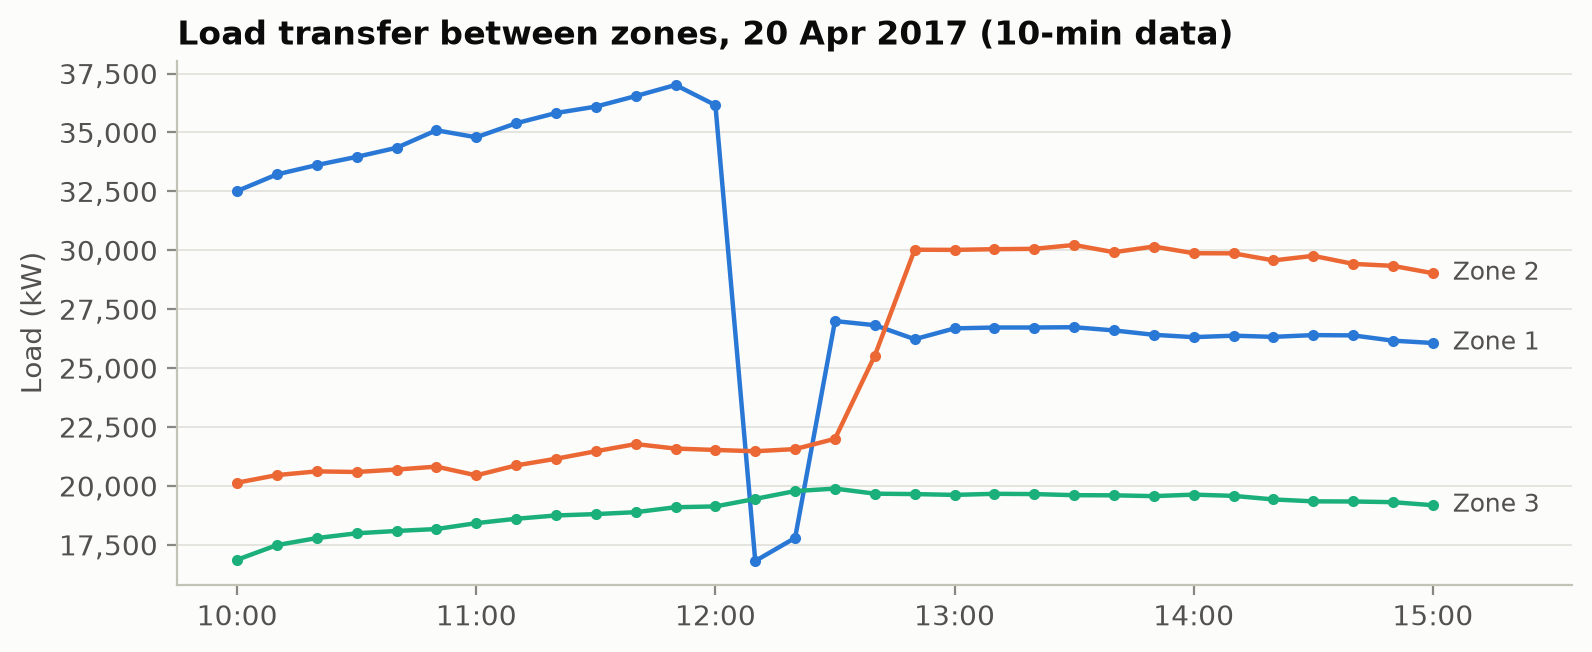
\includegraphics[width=\linewidth]{DQ01_zone_transfer_20170420.png}
\caption{Zone and total-load behavior around 20 April (DQ01). Redistribution between networks is a plausible interpretation; no independent operational log confirms it.}\label{fig:zone_event}
\end{figure}
\begin{figure}[tbp]\centering
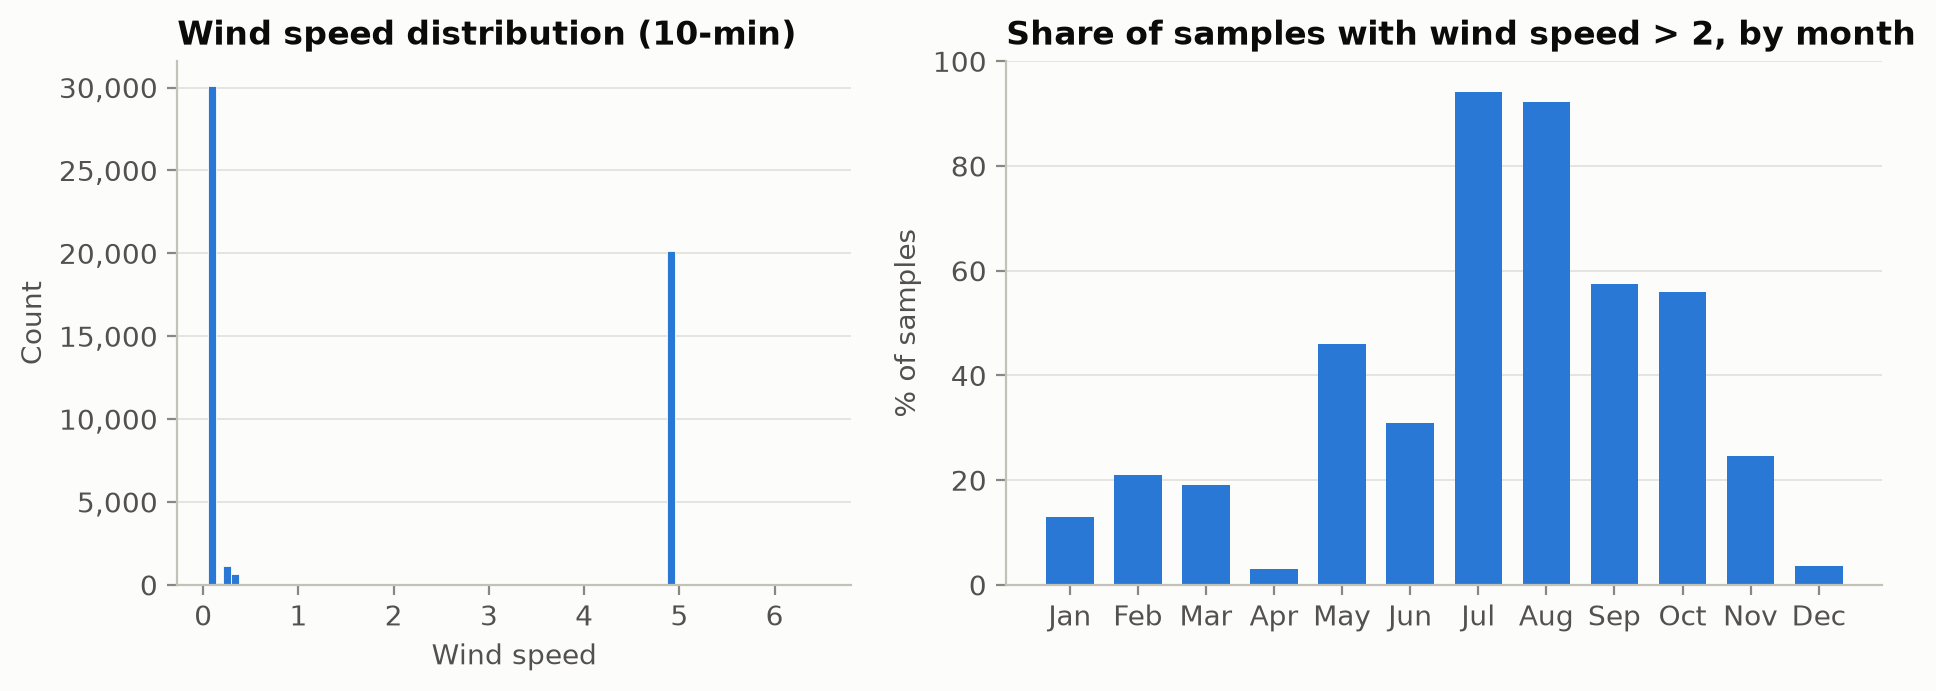
\includegraphics[width=.88\linewidth]{DQ02_windspeed_bimodal.png}
\caption{Whole-year wind-speed diagnostic (DQ02). The bimodal distribution motivates caution about sensor semantics; the pipeline retains the observed values. This descriptive graphic includes December.}\label{fig:wind}
\end{figure}
\begin{figure}[tbp]\centering
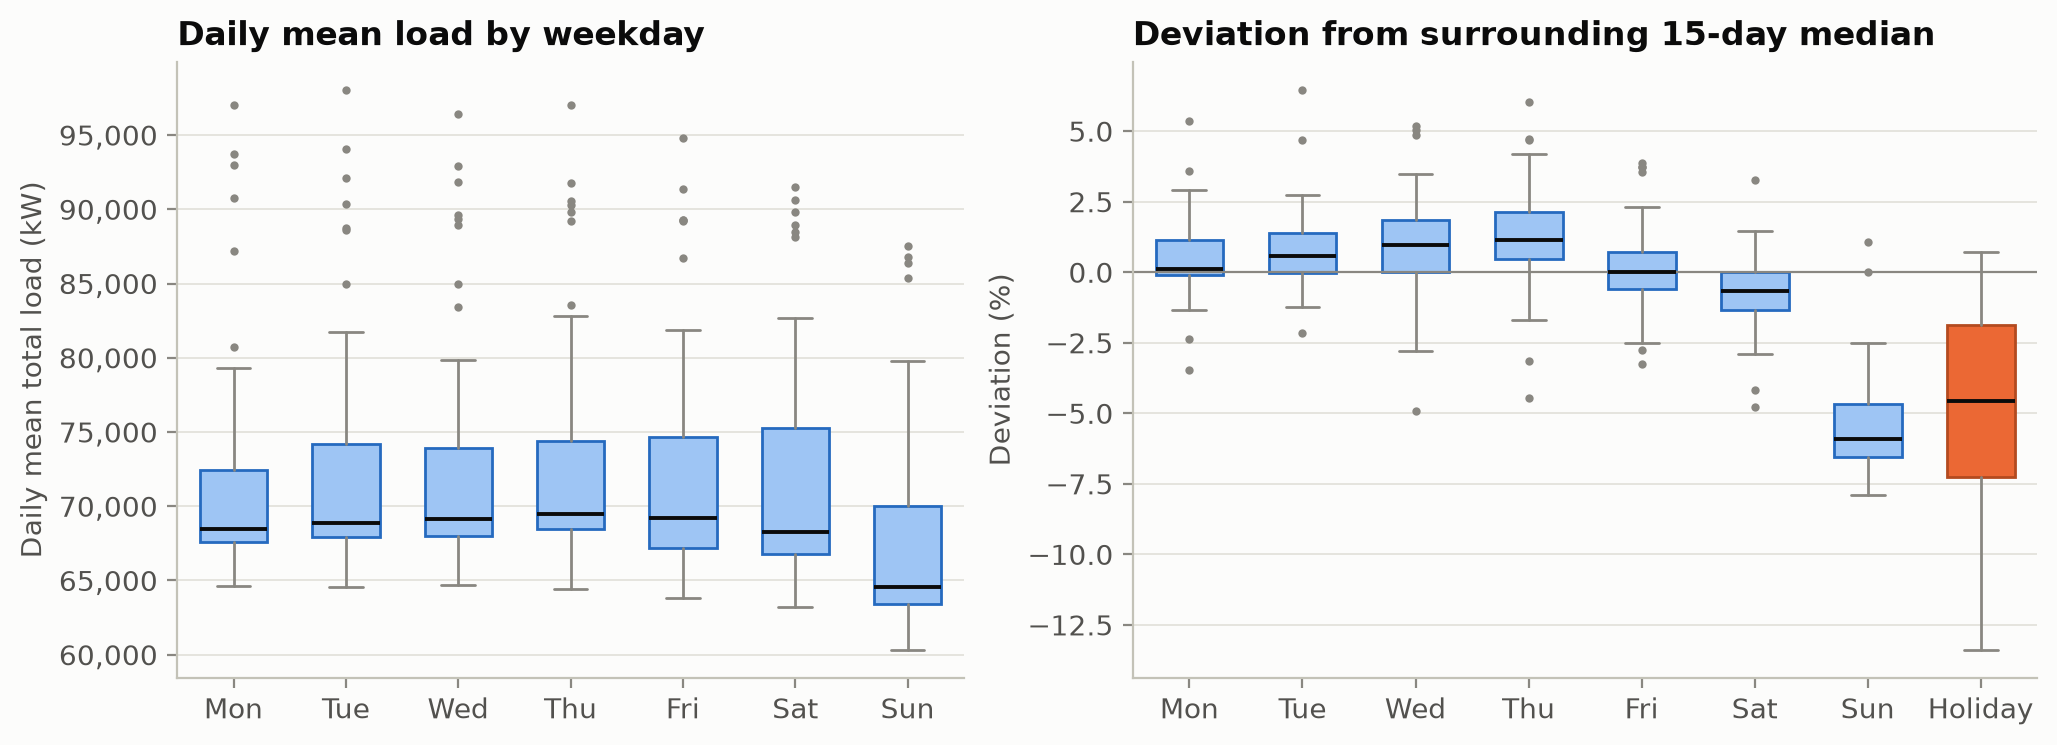
\includegraphics[width=\linewidth]{F08_weekday_holiday.png}
\caption{Development-period weekday and holiday load profiles (F08). Group differences motivate calendar predictors but are neither causal effects nor independently validated event forecasts.}\label{fig:holidays}
\end{figure}
\FloatBarrier

\Cref{fig:test_scatter} supplements the selected-SVR test analysis: most observations are close to the equality line, but local departures remain. \Cref{fig:shap_dependence} shows conditional associations within the residual RF. Its lag-24 contributions explain the learned correction and exclude the explicit lag base; its temperature pattern is not a causal demand-response estimate.
\begin{figure}[tbp]\centering
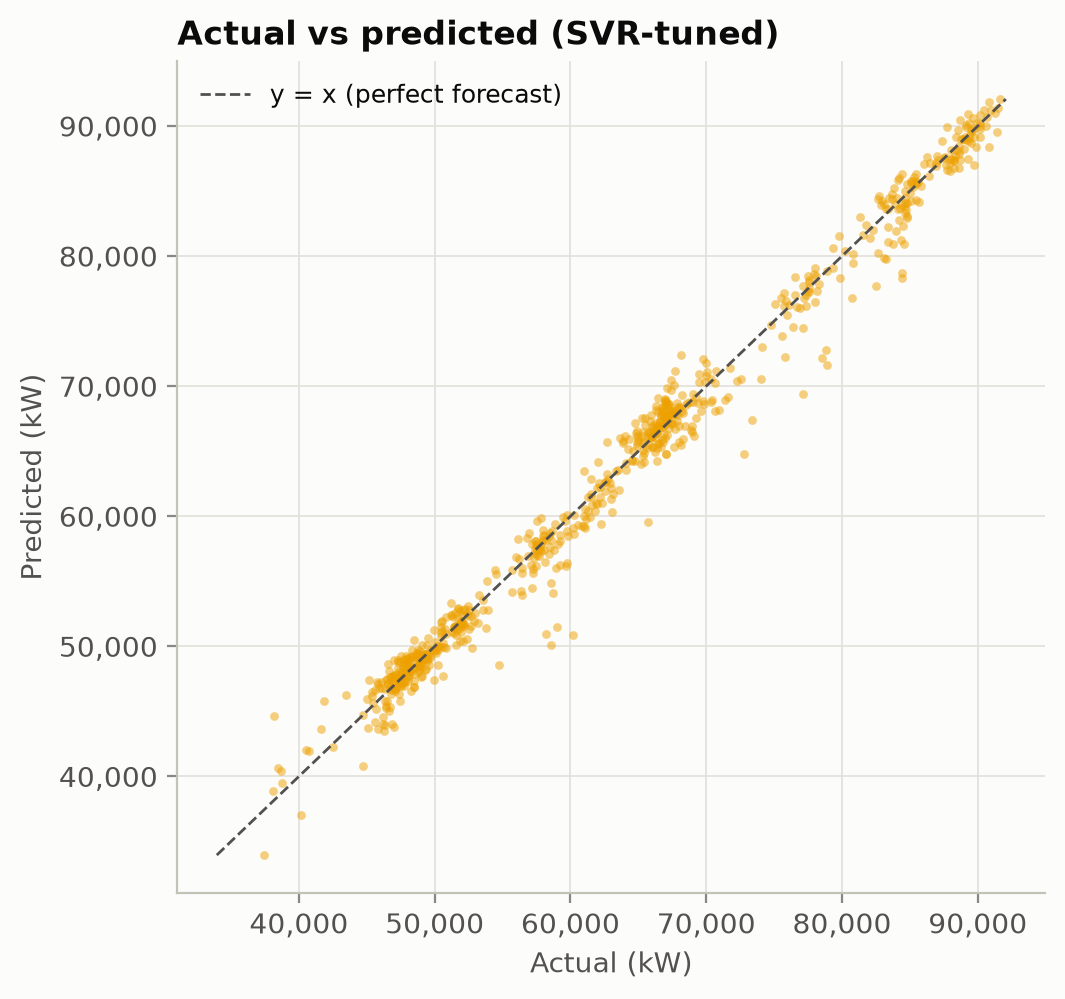
\includegraphics[width=.70\linewidth]{F17c_scatter.png}
\caption{Selected h24 SVR forecasts against actual December loads (F17c). The equality reference aids assessment of large local misses; proximity alone does not establish calibrated uncertainty or temporal independence.}\label{fig:test_scatter}
\end{figure}
\begin{figure}[tbp]\centering
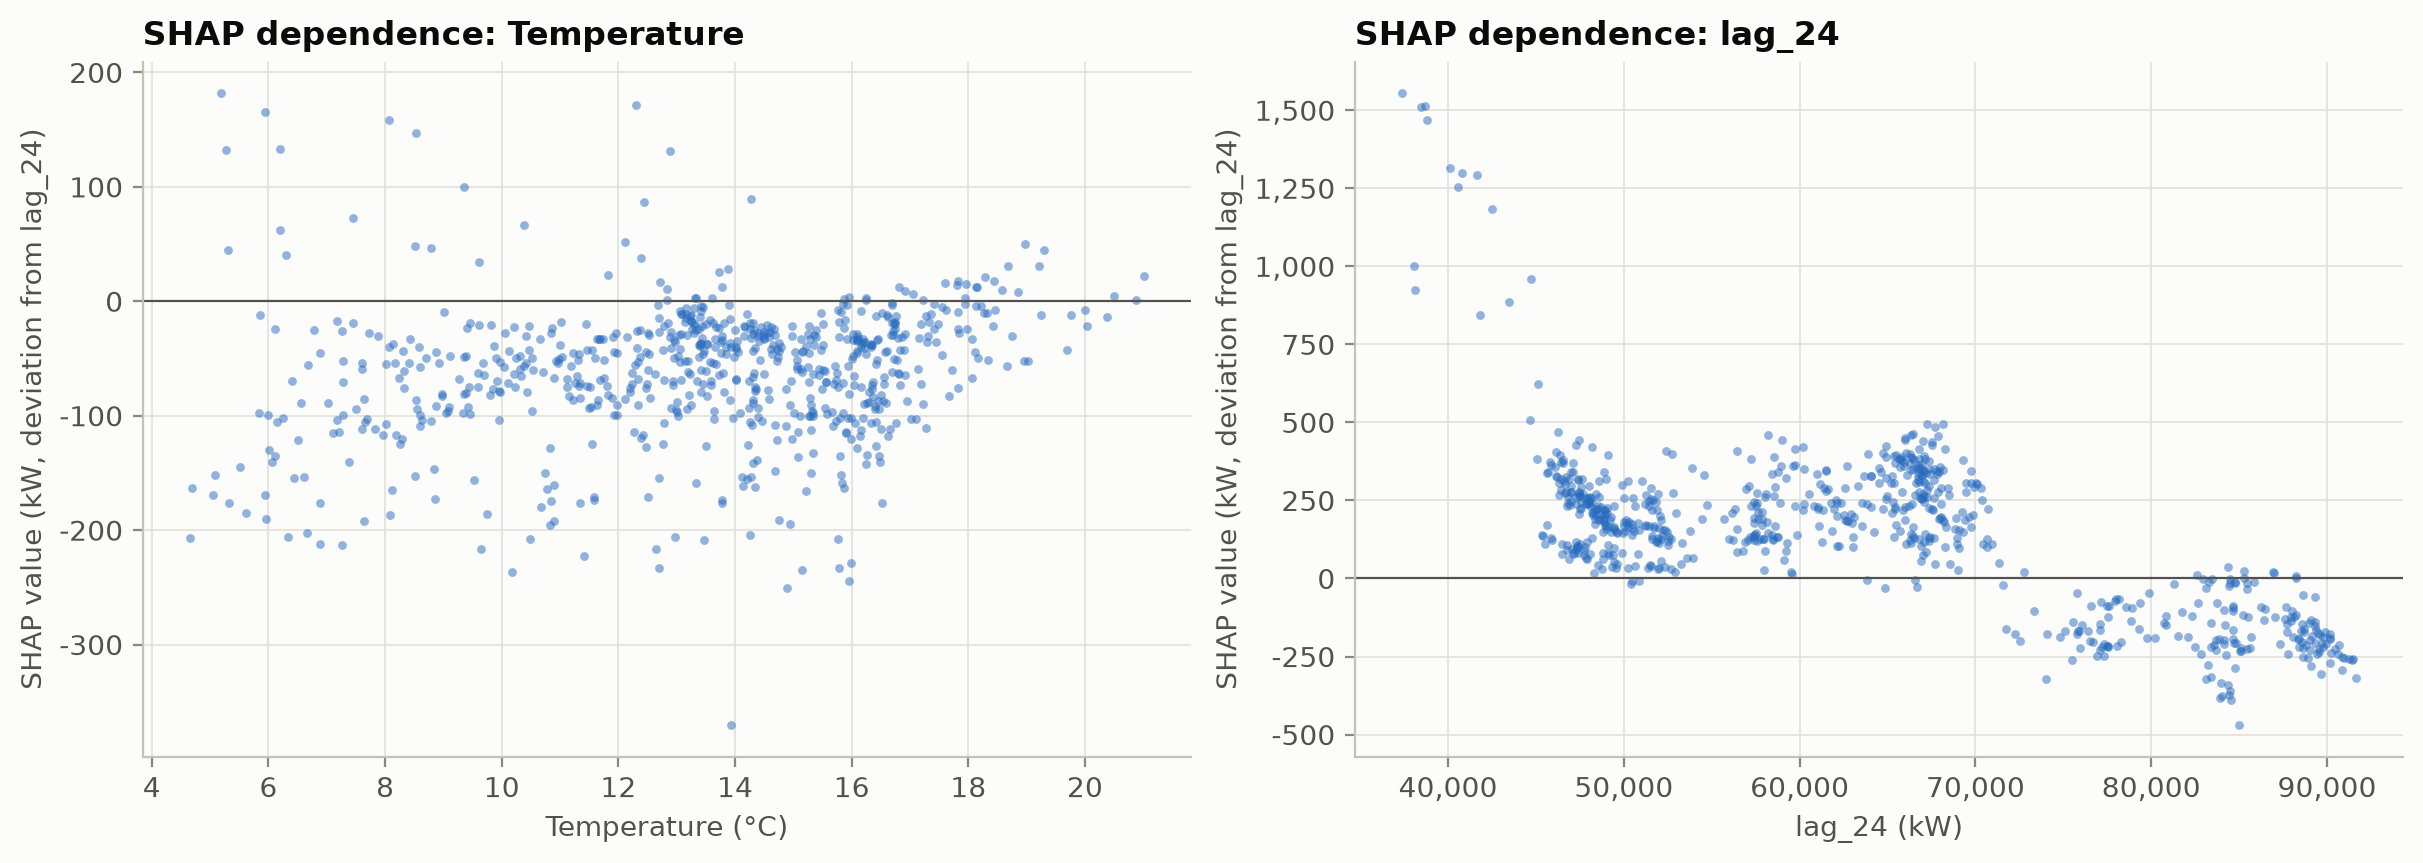
\includegraphics[width=\linewidth]{F19c_shap_dependence.png}
\caption{Residual-RF Tree SHAP dependence plots for temperature and lag-24 on December inputs (F19c). Values are contributions to the residual model output in kW, not to the separately added baseline.}\label{fig:shap_dependence}
\end{figure}
\FloatBarrier

\subsection{Unavailable artifacts and unresolved metadata}
The planned F09 pipeline graphic is absent; no replacement experiment output is invented. F14 is reviewed but omitted because its jointly varying parameters do not provide controlled single-parameter sensitivity. F20 is omitted to avoid visually ranking incompatible literature tasks. The related-work table and survey preserve the underlying contextual evidence instead.

Outstanding metadata include student/team names and IDs, instructor and submission date, wind/radiation units, timestamp timezone, measurement latency and detailed hardware configuration. The local row count differs from the dataset landing-page count. The literature review leaves certain paper targets, horizons and optimizer descriptions unresolved; these qualifications are retained in \cref{sec:related}. None prevents compilation, but they constrain the scientific interpretation and should be resolved before stronger claims or operational use.

\end{document}
